\section{Teoretická časť diplomovej práce}

\subsection{Počítačom generovaná realita}

Počítačom generovaná realita alebo \gls{xr} zahŕňa 3 typy realít, tými sú \gls{ar}, \gls{vr} a \gls{mr}. Snaží sa o zmenu našej reality rozšírením, virtualizovaním alebo miešaním realít naskladaním alebo vnáraním počítačového textu alebo grafiky do nášho reálneho sveta a virtuálneho sveta alebo do oboch naraz. 

\begin{figure}[h]
  \centering
  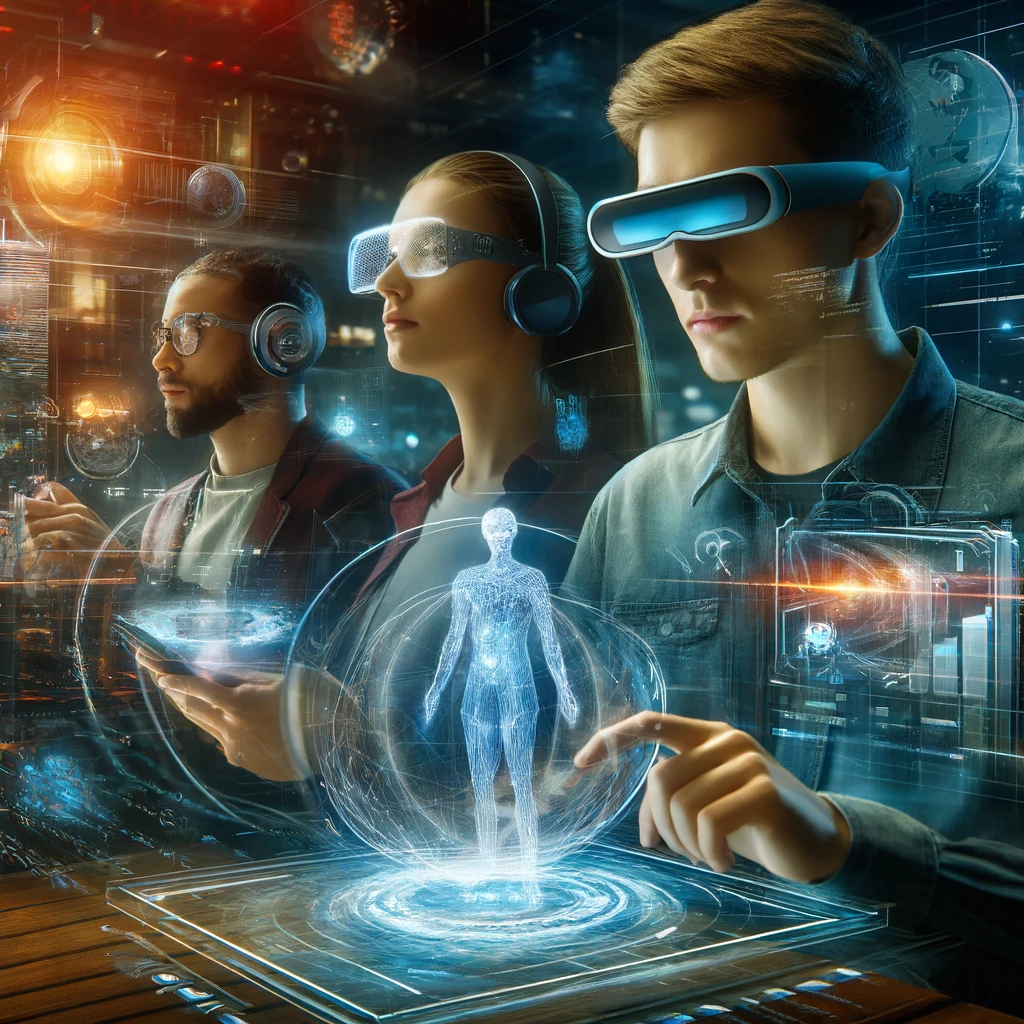
\includegraphics[width=0.6\textwidth]{img/Pocitacom_generovana_realita.png}
  \caption{Ilustrácia využitia počítačom generovaných realít (generované umelou inteligenciou s pomocou modelu DALL-E)}
  \label{fig:poc_gen_real}
\end{figure}

Všetky tieto 'reality' zdieľajú spoločné prekrývajúce sa rysy a požiadavky, každá má odlišné účely a základné technológie. xR hraje fundamentálnu rolu v~metaverse - ďalšej evolúciu internetu vďaka ktorej zlúčime reálny, digitálny svet a virtuálny svet do novej reality vďaka akejkoľvek dostupnej 'bráne' alebo teda prístroju, ako sú napríklad VR okuliare alebo \gls{ar} inteligentné okuliare \cite{armXR2022}. %EK: aky je rozdiel medzi virtualnym a digitalnym svetom? - PPRIDANE VYSVETLENIE NIZSIE

Digitálny svet je širším pojmom zahŕňajúcim všetku digitálnu komunikáciu a interakciu, virtuálny svet je konkrétnejší a zameriava sa na vytváranie imerzívnych, interaktívnych prostredí, ktoré simuluju realitu alebo fantastické svety v~trojrozmernej forme \cite{redkiwi2024digitalvirtual}.

Ako sme už spomínali, \gls{xr} technológie zdieľajú fundamentálne rysy, a to napríklad to, že základným kameňom všetkých nositeľných zariadení \gls{xr} je schopnosť používať vizuálne vstupné metódy, ako je sledovanie objektov, gest a pohľadu na navigáciu svetom a zobrazovanie kontextovo citlivých informácií. Hĺbkové vnímanie a mapovanie sú taktiež umožnené pomocou hĺbky a polohy. %EK: Zase je tu xR a potom XR. Treba zjednotit - ZMENENE NA xR

Taktiež môžeme extended reality nazývať aj pohlcujúcou technológiou \cite{armXR2022}. 

\begin{itemize}
    \item \textbf{AR (Rozšírená realita):} Superponuje digitálne objekty na reálny svet.
    \item \textbf{VR (Virtuálna realita):} Užívateľa úplne pohlcuje a prenáša do digitálneho sveta.
    \item \textbf{MR (Zmiešaná realita):} Kombinuje prvky AR a VR, čím umožňuje interakcie medzi reálnymi a virtuálnymi objektmi.
\end{itemize}

%PRIDANE 
Pre tieto 3 typy realít poznáme rôzne zariadenia, ktoré môžeme používať:

\begin{itemize}
\item \textbf{AR (Rozšírená realita):} AR môže byť použitá cez rôzne zariadenia, vrátane smartfónov, tabletov a \gls{hmd}. Táto technológia projektuje CGI (Computer-generated imagery), ako prekrytie na fyzický svet, pričom môže, ale nemusí úplne blokovať pohľad na okolité prostredie.
\item \textbf{VR (Virtuálna realita):} VR používa špeciálne HMD prístroje, ktoré izolujú užívateľa od fyzického sveta a nahrádzajú ho úplne digitálnym prostredím, zvyčajne prostredníctvom \gls{cgi} alebo 3D videozáznamov. Toto úplné pohltenie umožňuje intenzívne imerzívny zážitok.
\item \textbf{MR (Zmiešaná realita):} MR môže byť zobrazovaná cez HMD alebo mobilné zariadenia. Zariadenia používané pre MR sú schopné spracovávať a prispôsobovať sa fyzickým prekážkam v~prostredí, čím zabezpečujú plynulé zobrazenie a interakciu.
\end{itemize} %EK: AR mozeme sledovat aj cez HMD. Takisto MR mozeme sledovat aj cez mobil. Nie je to spravne napisane. Ked mam na hlave HoloLens a nemam nejake GUI naviazane na objekt ale niekde to je stale len pred ocami, tak je to AR. Takisto, ked mam mobil, tak nic nebrani tomu, aby digitalne objekty interagovali s virtualnymi, takze je to potom MR. Pozri si prednasku, ktoru sme mali na VZR alebo MTMP. - PREROBENE, pridane do MR aj mobilné zariadania, do AR pridané HMD

\cite{gonzalez2023what}

\subsubsection{Rozšírená realita - Augmented reality (AR)}

Rozšírená realita (AR) je integrácia digitálnych informácií s užívateľovým prostredím v~reálnom čase. Rozšírená realita je používaná na buď zmenu prirodzeného prostredia akýmkoľvek spôsobom, alebo na poskytovanie dodatočných informácií používateľovi. Primárnym benefitom rozšírenej reality je to, že dokáže zmiešať digitálne a trojdimenzionálne komponenty s individuálnym vnímaním reálneho sveta. Rozšírená realita má mnoho využitia napríklad od pomáhania v~rôznych situáciach a rozhodnutiach až po zábavu.

\begin{figure}[h]
  \centering
  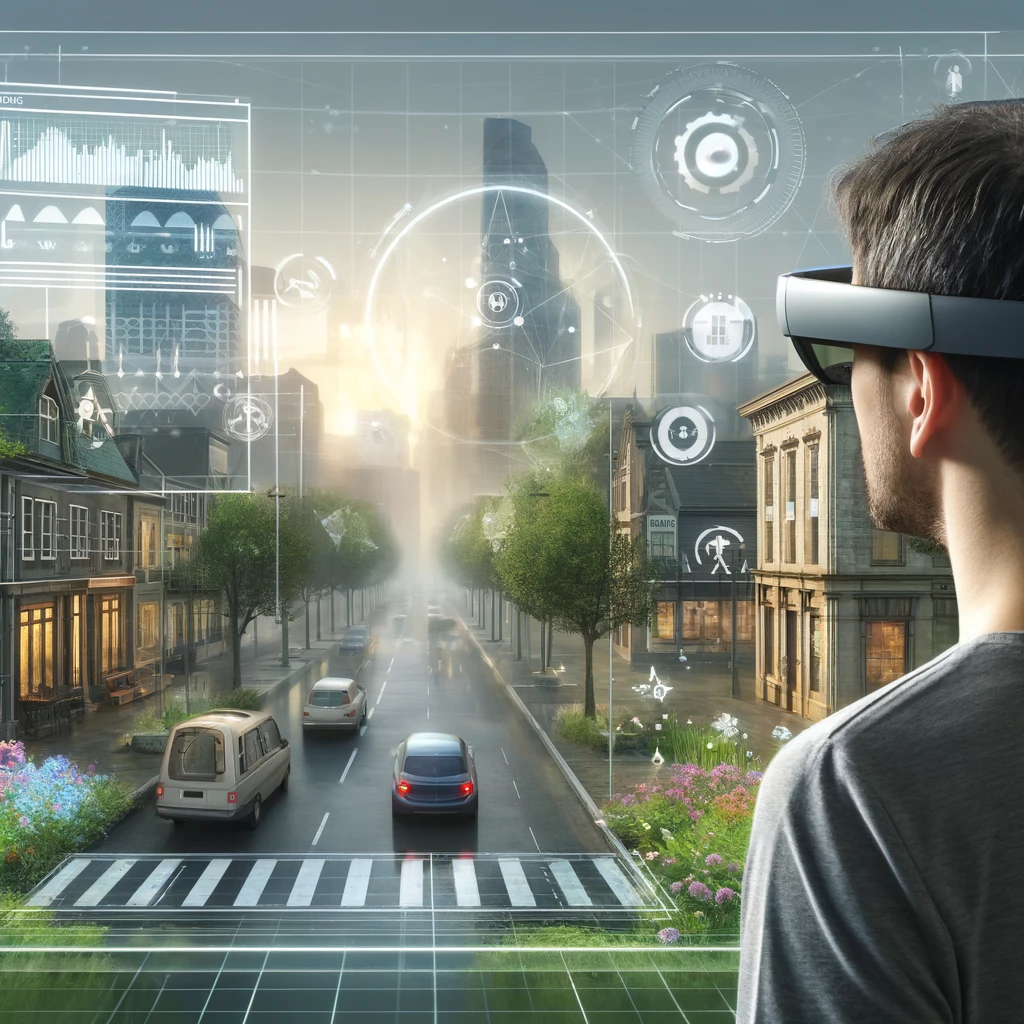
\includegraphics[width=0.5\textwidth]{img/rozsirena_realita.png}
  \caption{Ilustrácia použitia rozšírenej reality (generované umelou inteligenciou s pomocou modelu DALL-E)}
  \label{fig:roz_real}
\end{figure}

Rozšírená realita prináša vizuálne elementy, zvuky a iné senzorické informácie užívateľovi pomocou zariadenia, ako je napríklad telefón alebo inteligentné okuliare. Tieto informácie sú prekryté na zariadenie pre vytvorenie, aby mohli vytvoriť prepojený zážitok, ako v~reálnom svete avšak digitálna informácia ovplyvňuje a mení užívateľove vnímanie sveta. 

Zamestnanec Boeing Computer Services Research, Thomas Caudell, prvý krát použil názov rozšírená realita (augmented reality) v~roku 1990 pri opise náhlavného prístroja, ktorý používali elektrikári pri skladaní komplikovaných káblových zväzkov. Jedným z prvých komerčných aplikácií technológie rozšírenej reality bola žltý prvá línia, ktorá sa začala používať počas televíznych futbalových podujatiach niekedy v~roku 1998 \cite{gillis2024ar}. 

Dnes sa rozšírená realita používa v~Apple Vision, čo sú inteligentné okuliare od firmy Apple, v~mobilných telefónnych hrách a projekcie na čelných sklách automobilov sú najznámejšími konzumentskými produktmi rozšírenej reality. To však neznamená, že tam sa využitie rozšírenej reality končí. Táto technológia je používaná v~mnohých odvetviach vrátane zdravotníctva, verejnej bezpečnosti, plynárenskom a ropnom priemysle, turizme a marketingu. %PREROBENE

\subsubsection{Virtuálna realita - Virtual reality (VR)}

Virtuálna realita je simulácia 3D prostredia, ktorá umožňuje používateľovi objavovať a interagovať s virtuálnym prostredím spôsobom, ktorý sa čo najviac snaží napodobiť realitu, ako ju vnímame my, ako užívatelia cez naše zmysly. Prostredie je vytvorené počítačovým hardvérom a softvérom a požívatelia musia byť vybavený zariadením, ako je helma alebo okuliare na interakciu s virtuálnou realitou. 

Čím viac sa užívateľ snaží ponoriť do virtuálnej reality a izolovať sa od fyzického sveta, tým viac je ochotný akceptovať „realitu“ tohto prostredia, aj keď je toto „fantastické prostredie“ nereálne.

Priemysel okolo virtuálnej reality je stále ďaleko od realizácie vízie vytvorenia dokonalého virtuálneho prostredia, do ktorého keď zapojíme rôzne zmysly a  vnoríme sa do neho, nebudeme vedieť rozoznať skutočnosť a fiktívny svet. Avšak, technológia má ešte veľmi veľa nedostatkov v~poskytovaní takéhoto pocitu z virtuálnej reality, to však neznamená, že to nedokáže ani v~budúcnosti. Virtuálna realita má odhad na obrovské využitie v~rôznej škále priemyslov. 

Systémy virtuálnej reality sa líšia jeden od druhého signifikantným spôsobom, záležiac na ich spôsobe využitia a technológie, ktoré používajú. Všeobecne však patria do nasledujúcich troch kategórií: 

Non-immersive (ne-immerzívne) sú typ zariadení virtuálnej reality, ktorá odkazuje typicky na 3D simulované prostredie, ktoré je dostupne skrz počítačovú obrazovku. Prostredie môže taktiež generovať zvuk, to však záleží od programu. Užívateľ má nejakú kontrolu nad virtuálnym prostredím používaním klávesnice, myšky alebo iných zariadení, ale prostredie neinteraguje priamo s používateľom. Videohra je dobrým príkladom ne-imerzívneho typu virtuálnej reality, taktiež tu patrí napríklad aj webstránka, ktorá dovoľuje používateľovi nadizajnovať dekoráciu v~izbe. 

Semi-immersive (čiastočne imerzívny) typ virtuálnej reality ponúka čiastočný zážitok z virtuálnej reality, ktorý je prístupný cez počítačovú obrazovku alebo nejaký typ okuliarov alebo slúchadiel. Zameriava sa hlavne na vizuálne 3D aspekty virtuálnej reality a neinkorporuje fyzický pohyb v~zmysle, v~akom to dokáže len naozajstná realita. Bežným príkladom takejto čiastočne imerzívnej virtuálnej reality je simulátor lietania, ktorý sa používa v~leteckom a vojenskom priemysle na zaúčanie nových alebo trénovanie starších pilotov. 

Fully immersive (plne imerzívny) typ virtuálnej reality ponúka najlepší zážitok z virtuálnej reality, kompletne ponorený používateľ je v~simulovanom 3D prostredí. Inkorporuje zrak, zvuk a v~niektorých prípadoch aj hmat. Sú tu dokonca aj experimenty s~dodatočným zapojením čuchu. Používateľ má nasadené špeciálne zariadenie, ako je helma, okuliare alebo rukavice, ktoré sú schopné plne interagovať s prostredím.

Prostredie taktiež môže zahŕňať využitie bežiaceho pásu alebo stacionárnych bicyklov na poskytnutie používateľovi zážitok z pohybu skrz 3D svet. Plne imerzívna technológia virtuálnej reality je oblasť, ktorá je staré len v~zárodku, ale už dokázala preraziť do herného priemyslu v~nejakom slova zmysle aj do zdravotníckeho priemyslu a snaží sa zapájať do mnohá ďalších odvetví \cite{sheldon2022vr}.%EK: Skontrolovat sklonovanie - PREROBENE

\begin{figure}[h]
  \centering
  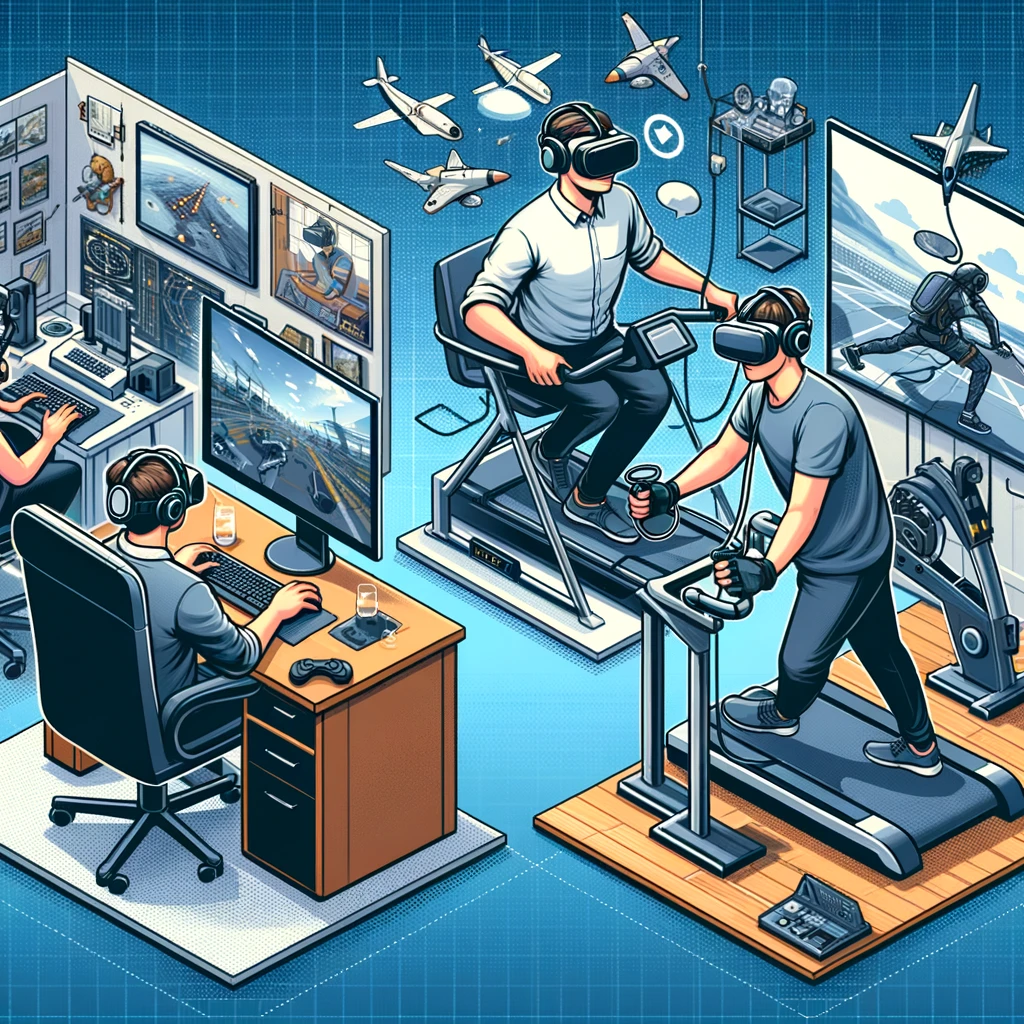
\includegraphics[width=0.5\textwidth]{img/virtualna_realita.png}
  \caption{Ilustrácia použitia virtuálnej reality (generované umelou inteligenciou s pomocou modelu DALL-E)}
  \label{fig:vir_real}
\end{figure}

\subsubsection{Zmiešaná realita - Mixed reality (MR)}

Ekosystém zmiešanej reality je pomaly sa vynárajúca technológia, ktorá začína byť na vzostupe a je záujem o jej vývoj čím ďalej tým viac. Je to technológia, ktorá poskytuje fyzickú a digitálnu interakciu limitovanú iba našou predstavivosťou. Zmiešaná realita je ďalšou vlnou v~oblasti počítačov hneď po mainframoch, počítačoch a smartfónoch. Zmiešaná realita sa pomaly stáva mainstreamom pre konzumentov a pre podniky. Oslobodzuje nás zo zážitkov viazaných na obrazovky poskytovaním inštinktívnej interakcie s dátami v~našom životnom priestore a s našimi priateľmi. 

Stovky miliónov ľudí po celom svete vyskúšali zmiešanú realitu prostredníctvom mobilných zariadení, čím sa stali akýmisi online prieskumníkmi novej technológie. Hoci mobilná rozšírená realita, ktorá je často používaná na sociálnych sieťach prostredníctvom filtrov, ako na Instagrame, primárne mení vizuálny vzhľad reálneho sveta, užívatelia možno ani nevedia, že skúsenosti s týmito filtrami sa približujú k zážitkom zo zmiešanej reality. Napríklad, technológia, ako Windows Mixed Reality poskytuje ešte pôsobivejšie holografické zobrazenia a 3D hologramy, ktoré užívateľom umožňujú nielen vidieť, ale aj interagovať so svetom okolo nich na úplne novú úroveň.

%Stovky miliónov ľudí po~celom svete mali, ako online prieskumníci možnosť zažiť zmiešanú realitu prostredníctvom prístrojov, ktoré sa držia v~ruke. Mobilná rozšírená realita, najrozšírenejšie dostupné riešenie doposiaľ, je často využívaná na~sociálnych sieťach. %PREROBENE %EK: Stale je to divne. Miesa sa rozsirena a zmiesana realita (aj ked potom dalej je to vysvetlene, ze AR filtre je znmiesana realita). Aki online prieskumnici? To je kto?

%Ľudia si často neuvedomujú, ale AR filtre, ktoré používajú na platformách, ako Instagram, vlastne predstavujú zážitok zo zmiešanej reality. Windows Mixed Reality tento zážitok posúva ešte ďalej s pôsobivými holografickými zobrazeniami ľudí, vysokou kvalitou 3D hologramov a možnosťou preskúmať svet okolo nás v~novom svetle.

\begin{figure}[h]
  \centering
  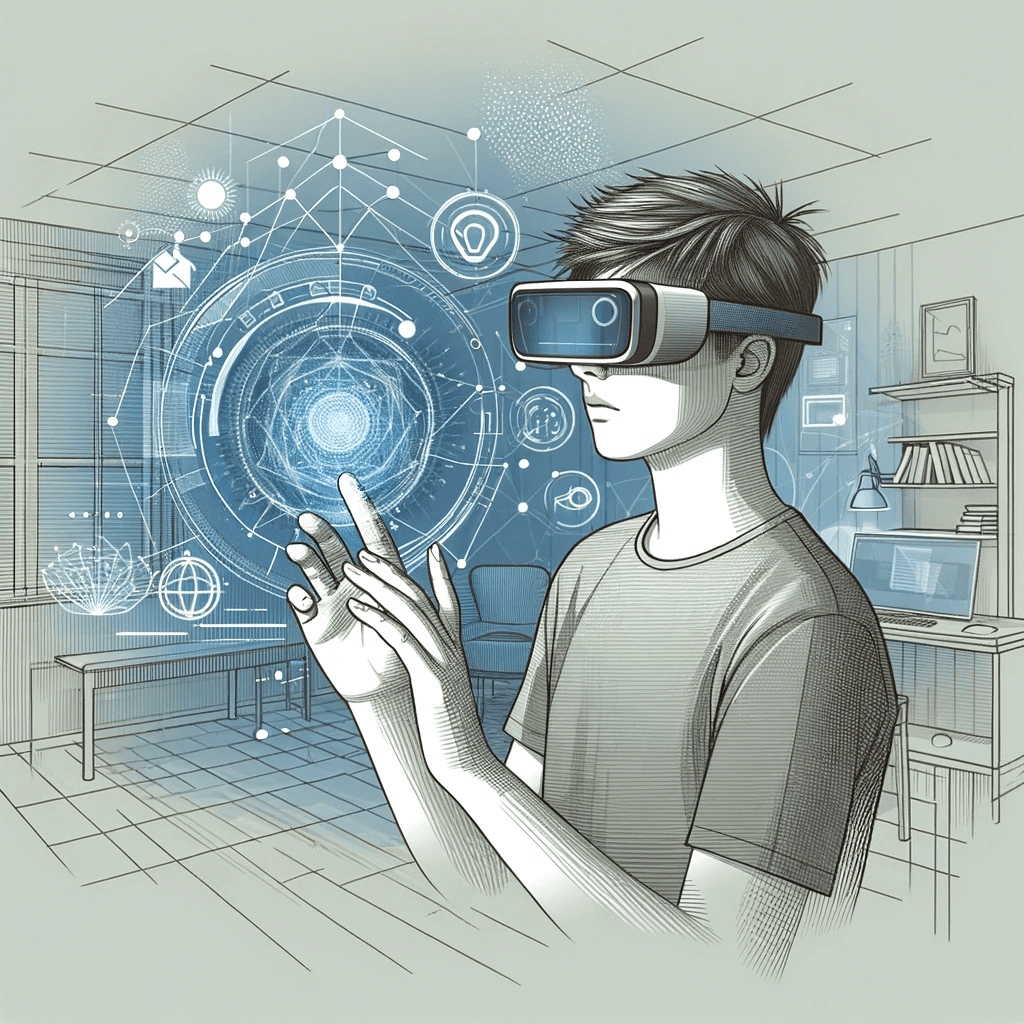
\includegraphics[width=0.5\textwidth]{img/zmiesana_realita.png}
  \caption{Ilustrácia použitia zmiešanej reality (generované umelou inteligenciou s pomocou modelu DALL-E)}
  \label{fig:mix_real}
\end{figure}

Zmiešaná realita kombinuje fyzický a digitálny svet, umožňujúc prirodzenú a intuitívnu 3D interakciu medzi ľuďmi, počítačmi a prostredím. Tento koncept je založený na~pokrokoch v~oblastiach, ako počítačové videnie, grafická analýza, displejové technológie, vstupné systémy a cloudové výpočty. Termín „zmiešaná realita“ bol prvýkrát použitý v~roku 1994 vedeckými autormi Paulom Milgramom a Fumio Kishinom vo~vedeckom článku s~názvom „A Taxonomy of Mixed Reality Visual Displays“. Ich práca sa zameriavala na~prieskum a vysvetlenie konceptov virtuálneho kontinua a klasifikácie vizuálnych displejov. Od tej doby sa zmiešaná realita rozšírila za~rámec displejov a teraz sa využíva v~rôznych aplikáciách. %PREROBENE

\begin{itemize}
    \item \textbf{Environmentálneho porozumenia:} priestorové mapovanie a kotvy
    \item \textbf{Ľudského porozumenia:} sledovanie rúk, sledovanie očí a hlasový vstup
    \item \textbf{Priestorového zvuku}
    \item \textbf{Lokácie a poziciovanie vo fyzických aj vo virtuálnych priestoroch}
    \item \textbf{Kolaborácie na 3D assetoch v~priestoroch zmiešanej reality}
\end{itemize}

V posledných dekádach sa vzťah medzi ľudmi a počítačmi postupne vyvíjal prostredníctvom vstupných metód, ktoré môžeme počítaču poskytnúť. Vznikla nová disciplína, ktorá je známa, ako interakcia človek-stroj alebo HCI (Human-computer interaction). Ľudský vstup môže teraz zahŕňať klávesnice, myš, dotyk, atrament, zvuk a Kinect skeletové sledovanie.

Kinect skeletové sledovanie je vývojový balíček s pokročilými senzormi, ktoré využívajú umelú inteligenciu. Poskytuje sofistikované počítačové videnie a hlasové modely. Zahŕňa v~sebe senzor hĺbky, priestorové mikrofónové pole s videokamerou a senzor orientácie, ako je všetko v~jednom malom zariadení s viac režimami, možnosťami a sadami pre vývoj softvéru. 

Pokroky v~oblasti senzorov a výpočtovej sile vytvárajú pre počítače nové typy vnímania prostredia založenom na pokročilých vstupných metódach. Toto je dôvod prečo API názvy, ktoré vo Windowse odhaľujú environmentálne informácie sa nazývajú percepčné \gls{api} \cite{microsoft2023mixedreality}.

\begin{table}[h]
\centering
\begin{tabular}{|l|p{7cm}|}
\hline
\textbf{Typ reality}       & \textbf{Vlastnosti}                                                                                                                                                                                                                             \\ \hline
Rozšírená realita (AR)     & Superponuje digitálne objekty na reálny svet, poskytuje dodatočné informácie a mení vnímanie okolia. Používa sa v~rôznych odvetviach, od pomoci v~situáciách až po zábavu. \\ \hline
Virtuálna realita (VR)     & Pohlcuje užívateľa do digitálneho sveta, poskytuje simuláciu 3D prostredia s využitím v~hernom priemysle a vo vojenskom tréningu.           \\ \hline
Zmiešaná realita (MR)      & Kombinuje prvky AR a VR, umožňuje interakcie medzi reálnymi a virtuálnymi objektmi. Využíva sa v~širokej škále odvetví.           \\ \hline
\end{tabular}
\caption{Porovnanie typov rozšírenej, virtuálnej a zmiešanej reality}
\label{tab:porovnanie_realit}
\end{table}

\subsection{Priemyselné revolúcie - história a súčasnosť}

\subsubsection{História}

Prvá priemyselná  revolúcia začala na konci 18-teho storočia, s mechanizáciou textilného priemyslu a vynálezom parného stroja. V~tomto období prebiehala tranzícia z agrárnej ekonomiky na priemyselnú ekonomiku, s parným strojom a mechanizáciou textilných fabrík hrala pivotnú rolu transformácia.

Druhá priemyselná revolúcia, ktorá sa začala v~neskorších rokoch 19-teho storočia a skorších rokoch 20-teho storočia. Bola charakterizovaná vývojom elektrickej energie a výrobnými linkami. Masová produkcia a elektrifikácia priemyslu revolucionizovala manufaktúry a vyrábanie produktov sa stalo viac dostupné a oveľa lacnejšie.

Tretia priemyselná revolúcia, často spomínaná, ako digitálna revolúcia sa objavila v~neskorších rokoch 20-teho storočia. Táto perióda bola poznačená rozšíreným používaním počítačov, internetu a automatizáciou. Tieto technológie vylepšovali komunikáciu a zefektívnili procesy, čo výrazne ovplyvnilo rôzne priemyselné podniky \cite{rajan2023industry40}. 

\subsubsection{Súčasnosť - Industry 4.0}

Známa aj, ako štvrtá priemyselná revolúcia, reprezentuje signifikantný rozdiel v~tom, ako funguje priemysel a ako sa vytvárajú produkty. Je charakterizovaná integráciou digitálnych technológií, dátami a IoT (Internet of Things) v~rámci tradičného výrobného procesu. Industry 4.0 nie je iba o automatizovaní rôznych úloh, ale vytváranie hlboko prepojeného a inteligentného systému, ktorý môže robiť rozhodnutia sám o sebe. Niektoré kľúčové technológie, ktoré poháňajú Industry 4.0 zahŕňajú umelú inteligenciu, strojové učenie, big dáta a pokročilá robotika \cite{rajan2023industry40}. 

Tento koncept alebo súbor technológií založený na troch predchádzajúcich revolúciách, Industry 4.0 nás vedie do novej éry výroby. Buduje na digitalizácii a automatizácií tretej revolúcie, ale posúva to na novú úroveň. V~tejto kapitole si povieme o kľúčových vlastnostiach Industry 4.0 a stručne ich popíšeme.%EK: I 4.0 nie je technologia, ale koncept alebo subor technologii a ich vyuzitie - ZMENENE NA Tento koncept alebo súbor technológií založený na troch

\begin{itemize}
    \item \textbf{Konektivita} - Najlepšie sa Industry 4.0 darí pod hlboko prepojených systémoch. Stroje a zariadenia komunikujú medzi sebou v~reálnom čase pre neustálu výmenu informácií a dátovej analýzy.
    
    \item \textbf{Dáta a analýza} - Dáta sú základným kameňom Industry 4.0. Informácie sú zbierané z rôznych zdrojov a na analýzu sa využívajú pokročilé analytické nástroje, ktoré dovoľujú výrobcom vytvárať informované rozhodnutia na optimalizáciu procesov.
    
    \item \textbf{Inteligentná výroba} - Inteligentné fabriky sú vybavené strojmi, ktoré môžu robiť autonómne rozhodnutia na základe predom poskytnutých inštrukcií. Inteligentné stroje sú vysoko adaptabilné a môžu sa prispôsobovať veľmi jednoducho meniacim sa požiadavkám a podmienkam.
    
    \item \textbf{Prispôsobenie a efektivita} - S pokročilými technológiami môžu výrobcovia produkovať vysoko prispôsobené produkty. Tieto poskytujú dobré zázemie pre vysoko volatilný trh, ktorý je ovplyvňovaný dopytom po personalizovaných tovaroch.
\end{itemize}

Kľúčovými vlastnosťami Industry 4.0 je 7 kategórií, ktoré riešia jednotlivé prvky, pre vylepšenie výroby. 

\begin{itemize}
   \item \textbf{Funkcionálne požiadavky}
   
   \begin{itemize}
     \item \textbf{Kyberneticko-fyzikálne systémy (CPS)}
        \begin{itemize}
            \item Jadrom Industry 4.0 je integrácia fyzických strojov s inteligentnými digitálnymi systémami, čo umožňuje monitorovanie, analýzu a kontrolu nad priemyselnými procesmi.
        \end{itemize}
     \item \textbf{Internet of Things (IoT)}
        \begin{itemize}
            \item IoT zariadenia zbierajú dáta z výrobných strojov a senzorov, čo umožňuje efektívne rozhodovanie, predikciu údržby a zlepšenie celkového výkonu.
        \end{itemize}
     \item \textbf{Big Data a analýza}
        \begin{itemize}
            \item Masívny počet dát je generovaných a pokročilé analýzy sú používané na získavanie dôležitých poznatkov z týchto dát. Tieto informácie pomáhajú optimalizovať produkciu a kvalitu.
        \end{itemize}
     \item \textbf{Strojové učenie a umelá inteligencia}
        \begin{itemize}
            \item Tieto technológie sú využívané na vývoj samo učiacich sa systémov, ktoré sa dokážu adaptovať a postupne optimalizovať operácie.
        \end{itemize}
     \item \textbf{Technológia digitálneho dvojčaťa}
        \begin{itemize}
            \item Vytvára virtuálnu reprezentáciu fyzických aktív, čo umožňuje simulácie, testovanie a predikovanie údržby.
        \end{itemize}
     \item \textbf{Cloud computing}
        \begin{itemize}
            \item Cloud umožňuje jednoduché ukladanie, dostupnosť a zdieľanie dát počas celého výrobného procesu a reťazca.
        \end{itemize}
     \item \textbf{Inteligentné továrne}
        \begin{itemize}
            \item V~inteligentných továrňach sú stroje, produkty a systémy silne integrované, čo umožňuje ich vzájomnú komunikáciu a spoluprácu na~dosiahnutie optimalizácie výrobných procesov. %PREROBENE TU
            %\item Sú to vysoko prepojené zariadenia, kde stroje, produkty a systémy komunikujú a kooperujú medzi sebou.%EK: Preformulovat. Nedava to zmysel
        \end{itemize}
   \end{itemize}
\end{itemize}

Industry 4.0 má veľký dopad na globálnej mierke. Vedie k viac efektívnemu a flexibilnému výrobnému procesu. Redukuje prestoje (výpadky prevádzky), zvýšenie personalizácie produktov a znižuje náklady. Tento posun nielen, že transformoval výrobný sektor, ale taktiež vytvoril priestor pre nové pracovné príležitosti v~technológiách a odbore dátovej analýzy \cite{rajan2023industry40}. 

V článku \textit{Pandemic, War, Natural Calamities, and Sustainability: Industry 4.0 Technologies to Overcome Traditional and Contemporary Supply Chain Challenges} popisujú, ako kvôli mnohým problémom a úskaliam, ktoré museli podniky čeliť, ako napríklad vojna, prírodné katastrofy, zvýšené množstvo smogu, pandémia museli podniky nájsť nové riešenia pri problémoch s logistikou a výrobou. Vďaka aplikácií Industry 4.0 technológií, ako je umelá inteligencia, IoT, Big data a analýzu, blockchain, automatizáciu a robotizáciu liniek a mnohé iné vymoženosti vďaka štvrtej priemyselnej revolúcii sa zvýšila úspešnosť prežitia a zvýšila sa miera produktivity a tým aj ziskovosti podniku.

Štúdia ukazuje, že aj keď je veľmi náročné predpovedať alebo detegovať úroveň narušenia zásobovania počas globálneho eventu, ale možnosť sa pripraviť a budovať dostatočne rezilientnú (odolnú) logistiku je v~záujme každého podniku, ktorý sa chce presadiť na dnešnom trhu. Existuje obrovské množstvo problémom, ktoré môžu podniky čeliť a k obrovskému množstvu riešení sa vieme dopracovať práve vďaka štvrtej priemyselnej revolúcie Industry 4.0 \cite{rajasanthi2022industry40}. 

Industry 4.0, ako poslednou kapitolou (zatiaľ) v~pokračujúcej ságe priemyselných revolúcií buduje na inováciách z minulosti. Prináša prepojenosť, dátami poháňajúce vykonávanie rozhodnutí a inteligentné továrne do popredia. Integrácia technológií vo výrobnom sektore je dynamický proces a Industry 4.0 je testament neustále sa vyvíjajucého sa ekosystému priemyslu \cite{rajan2023industry40}. 

\begin{figure}[h]
    \centering
    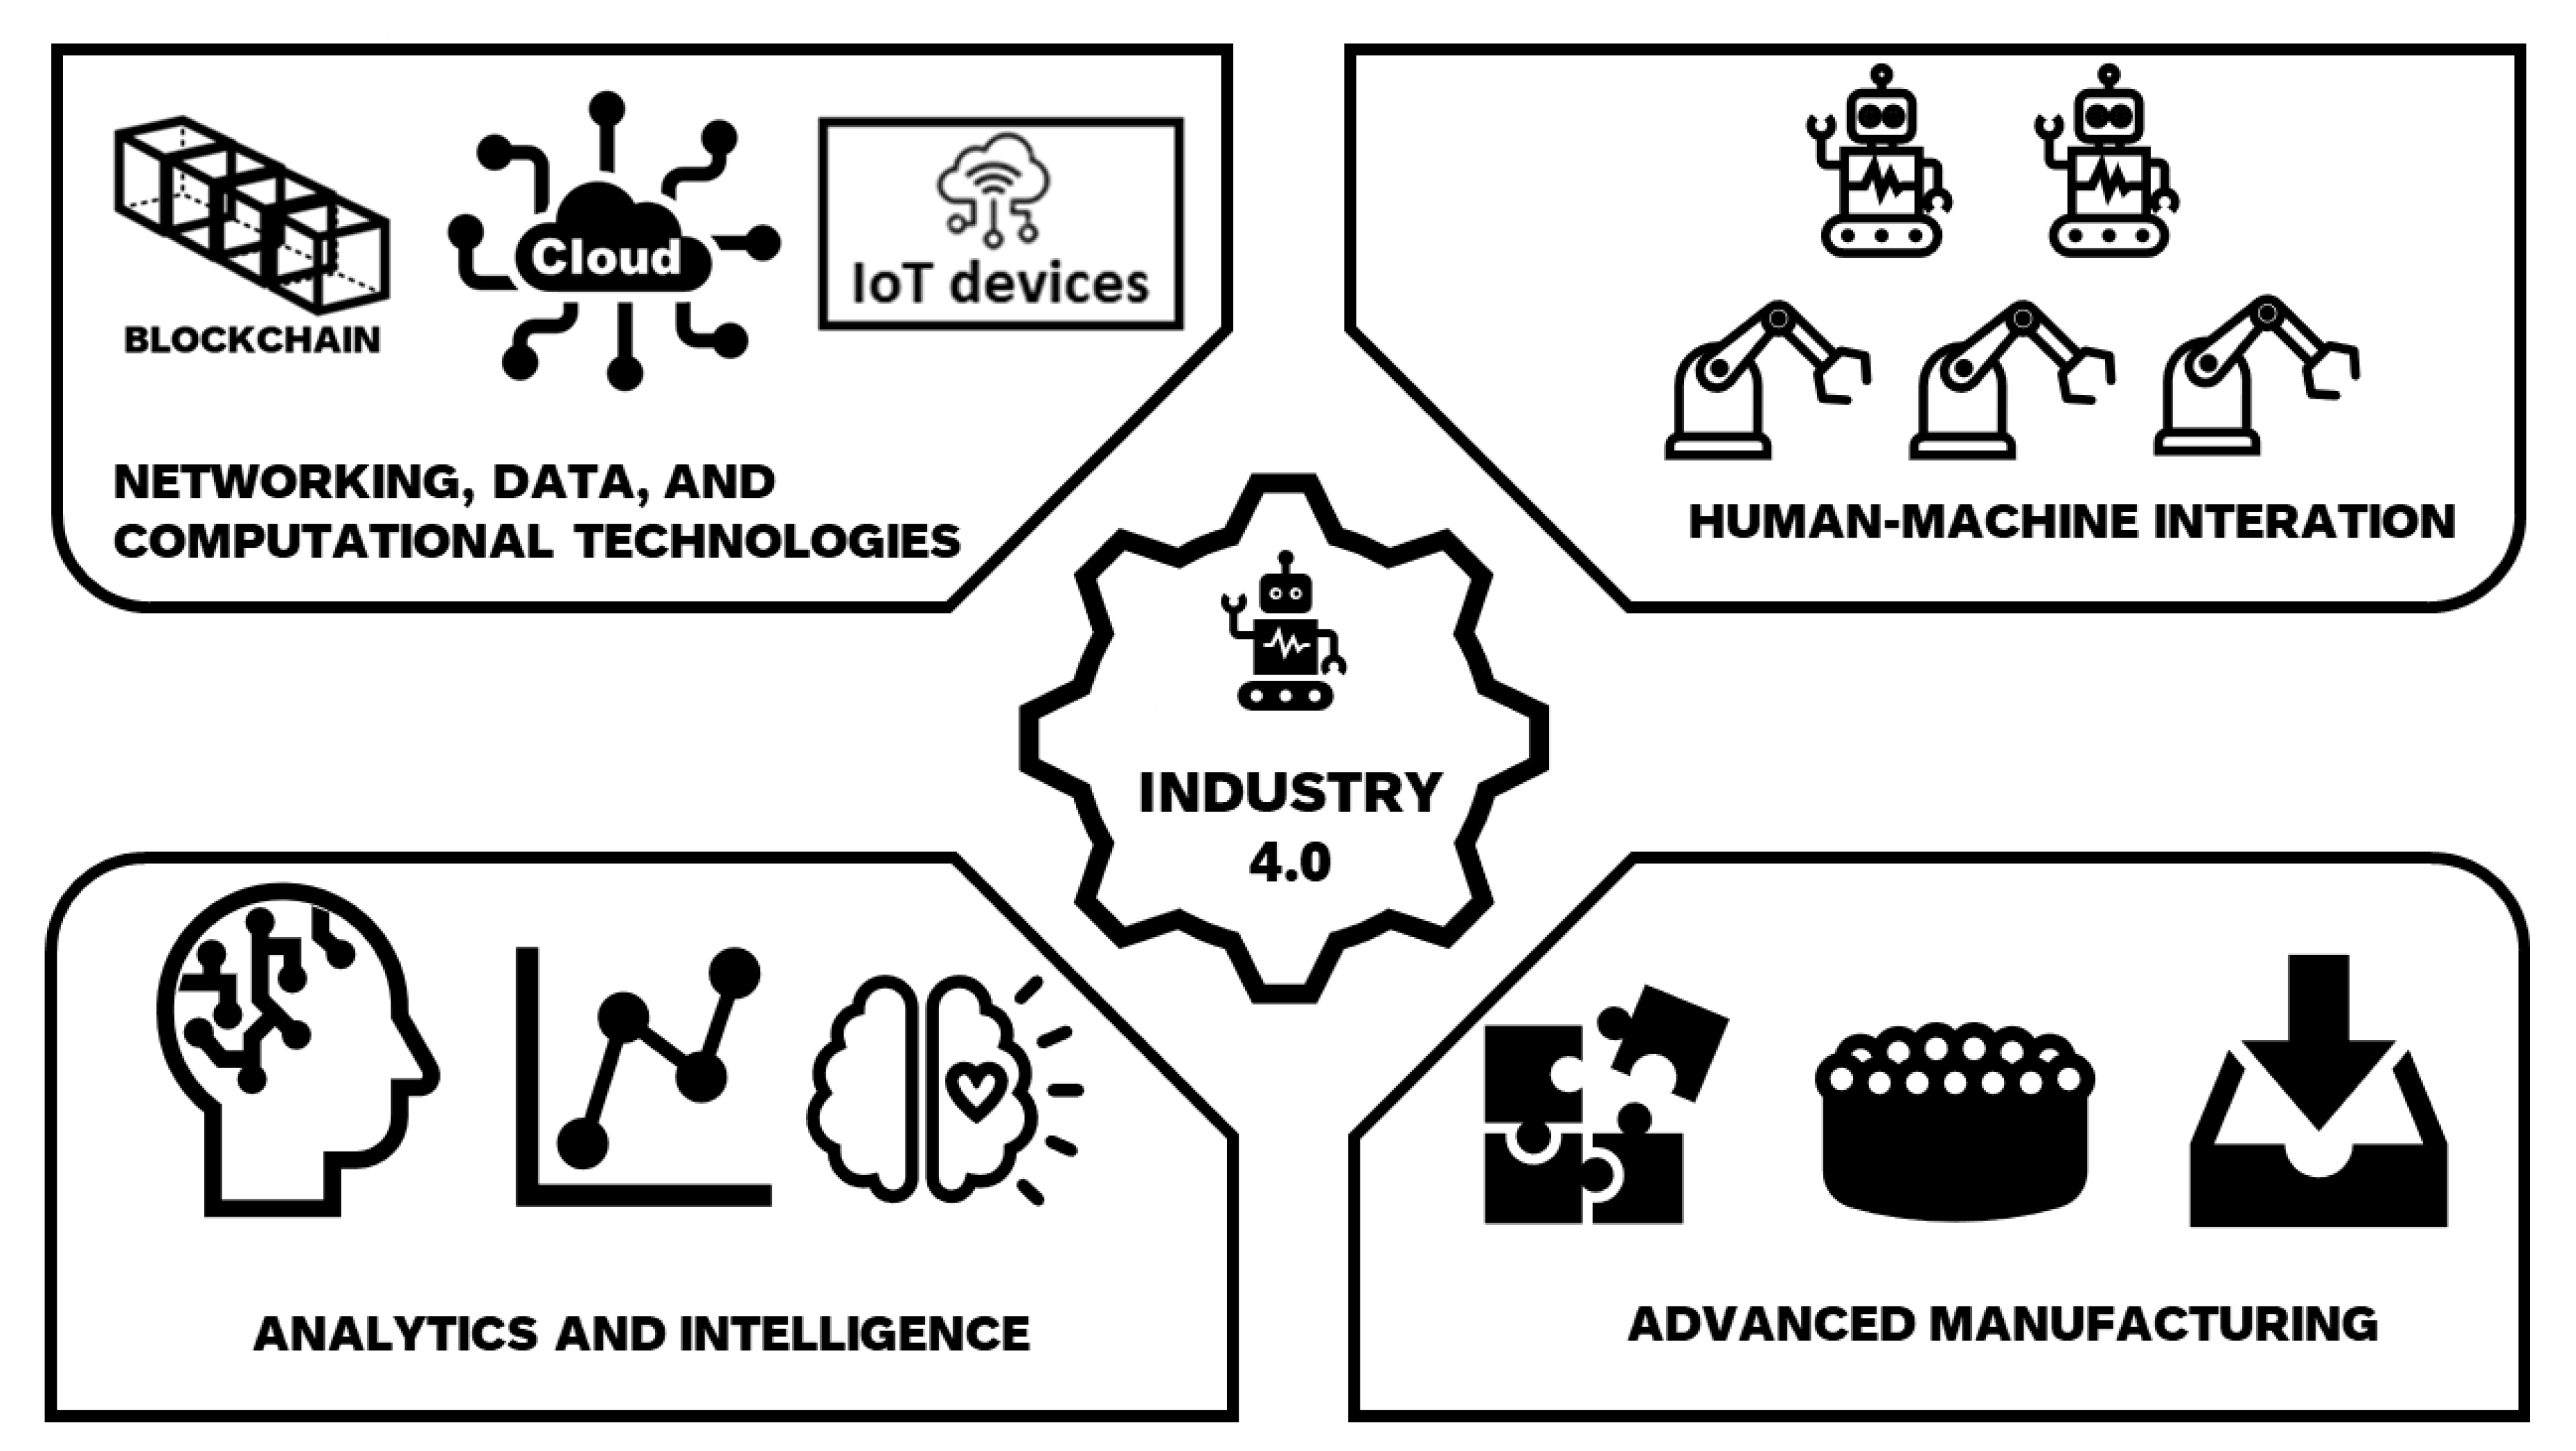
\includegraphics[width=1\textwidth]{img/logistics-06-00081-g003.png}
    \caption{Supply Chain Ecosystem and Industry 4.0 Technologies \cite{rajasanthi2022industry40}}
    \label{fig:industry40}
\end{figure}

\subsubsection{Budúcnosť - Industry 5.0}

Industry 5.0 predstavuje evolúciu od predchádzajúcich priemyselných revolúcií s dôrazom na spoluprácu medzi ľuďmi a inteligentnými systémami. Táto piata priemyselná revolúcia sa zameriava na personalizáciu výroby v~harmónii so záujmami a potrebami ľudských pracovníkov, čo predstavuje posun od automatizácie k personalizácii a udržateľnosti.

\begin{itemize}
\item \textbf{Pozadie vzniku}: v~reakcii na potreby vyššej personalizácie a zároveň udržateľnosti, Industry 5.0 prináša technológie, ktoré umožňujú podnikom lepšie sa prispôsobiť individuálnym požiadavkám zákazníkov a zároveň minimalizovať ekologickú stopu.

\item \textbf{Paradigmy}: Kľúčové paradigmy zahŕňajú humanizáciu automatizovaných procesov, zvýšenie adaptability výrobných systémov a integráciu udržateľných prístupov do všetkých aspektov výroby.

\item \textbf{Technológie a aplikácie}: Medzi hlavné technológie patria pokročilá robotika, umelá inteligencia a digitálne dvojčatá, ktoré sú navrhnuté tak, aby efektívne spolupracovali s ľudskými operátormi a zároveň poskytovali personalizované a optimalizované výrobné procesy.

\item \textbf{Implikácie pre priemysel}: Industry 5.0 nielenže posilňuje interakciu medzi človekom a strojom, ale tiež umožňuje podnikom rýchlejšie a efektívnejšie reagovať na meniace sa trhové podmienky a zákaznícke preferencie, čím prispieva k zvýšenej konkurencieschopnosti a inovatívnosti.

\end{itemize}

Tento posun k Industry 5.0 signalizuje dôležitú zmenu v~myslení priemyselných podnikov, kde sa zameranie na čistú efektivitu a automatizáciu prelína s potrebou udržateľnosti a zvýšenej spolupráce medzi človekom a strojom.

\begin{figure}[h]
\centering
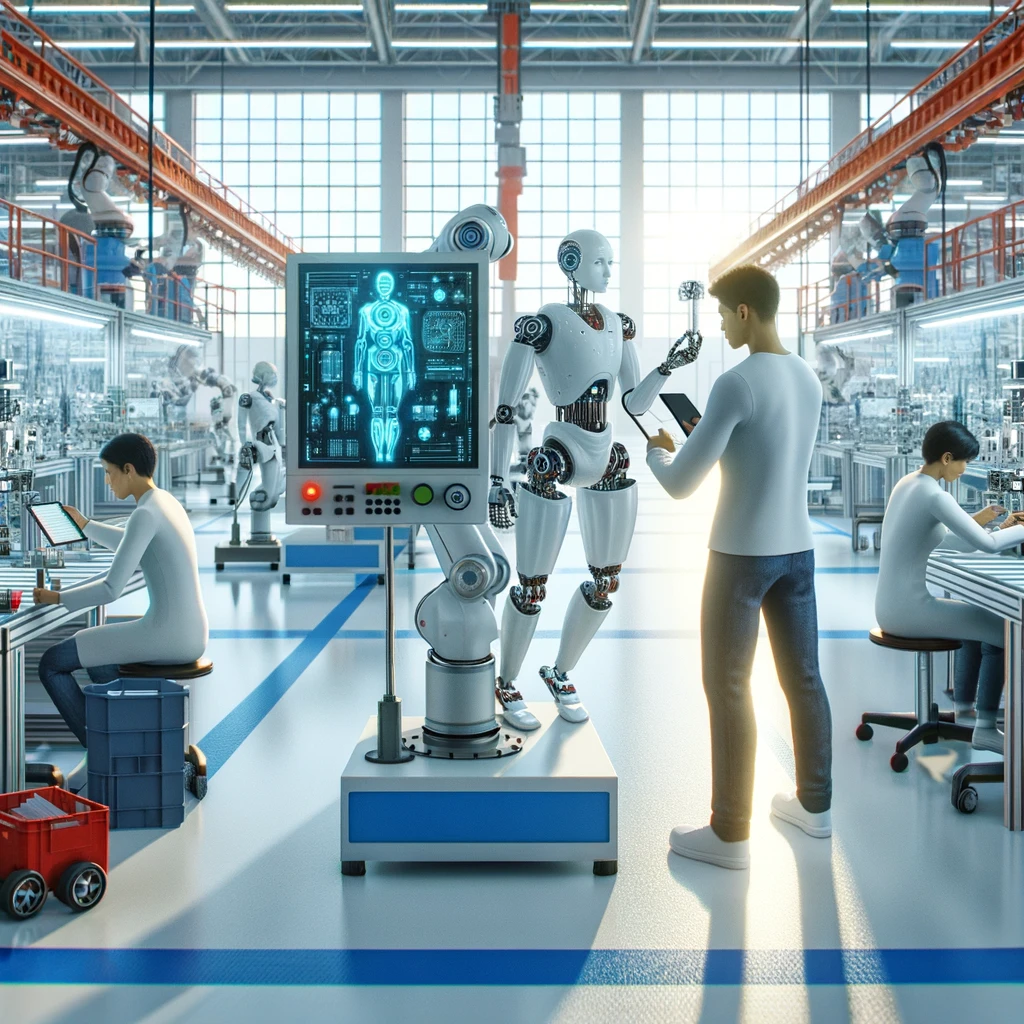
\includegraphics[width=0.6\textwidth]{img/industry_5.0.png}
\caption{Ilustrácia Industry 5.0 (generované umelou inteligenciou s pomocou modelu DALL-E) \cite{kucera2024industry40}}
\label{fig:unrealengine5}
\end{figure}

Industry 5.0 tak otvára nové horizonty pre podniky, ktoré hľadajú udržateľné a zákazníkmi riadené výrobné riešenia \cite{kucera2024industry40}. 

\section{Softvérové a hardvérové prostriedky}

\subsection{Herné enginy a modelovacie prostredia}

Herné enginy sú unikátnym prostriedkom pre vytváranie hier, animácií, aplikácií, a tak ďalej. Je to vývojové prostredie s nástrojmi, ktoré optimalizáciami uľahčujú development skrz rôzne programovacie jazyky. Takéto enginy môžu obsahovať buď 2D, 3D grafický rendering alebo oboje, ktorý je kompatibilný s rôznym typom formátov \cite{arm_gaming_engines}.  %EK: Mozu alebo musia? - PRIDANE môžu obsahovať buď jedno, druhe alebo oboje

V súčasnej dobe je najpopulárnejším herným enginom podľa hier, ktoré boli vydané na Steame, Itch.io, Unreal Engine a Unity. Okrem týchto bližšie opíšeme aj Godot v~ďalších kapitolách. Radi by sme upozornili na menej známe herné enginy, ako je CryEngine, ktorý sa preslávil vďaka hre Crysis a jej pokračovaniam. Rovnako by sme spomenuli aj Frostbite engine od spoločnosti Dice, ktorý získal popularitu vďaka sérii vojenských videohier z pohľadu prvej osoby, ako je Battlefield. V~dnešnej dobe si mnoho hlavne herných firiem vyrába svoje vlastné enginy, aby nemuseli platiť časti zvyškov zo svojich hier. Tieto čiastky sa môžu vyšplhať do výšky niekoľkých miliónov, ak sa jedna o AAA hru \cite{perforce2023gameengines}.  %PREROBENE

Grafické modelovacie prostredie je softvér, ktorý nám umožňuje modelovanie 3D objektov alebo prípadne 2D obrázkov. My sa budeme bližšie zaoberať hlavne tými, ktoré poskytujú 3D možnosti modelovania. 3D modelovanie je teda počítačový grafický proces vytvárania matematickej reprezentácie trojdimenzionálnych objektov alebo tvarov používaním špeciálneho softvéru. Digitálnou kópiou fyzického objektu nazývame 3D model a sú používané skrz rôzne priemyselné odvetvia. 

Medzi najznámejšie patrí Blender, Autodesk Maya, SketchUp, Cinema 4D, Autodesk, Creo Parametric a ďalšie. Limitované možnosti poskytuje avšak aj Unity herný engine \cite{autodesk2024modelingsoftware}. 

\subsubsection{Unreal Engine}

Unreal Engine je herným vývojovým prostredím. Bol vytvorený firmou Epic Games v~roku 1988 na vývoj video hier z pohľadu prvej osoby. V~dnešnej dobe je však využívaný na vytváranie rôznych iných typov žánrov, ako je RPG, MMORPG, a tak ďalej. Používa programovací jazyk C++. V~dnešnej dobe čím ďalej tým viac ľudí sa začína zaujímať o Unreal Engine hlavne aj vďaka novým updatom, ktoré vydávajú pomerne často s veľmi dobrým ohlasom. %EK: Unreal Engine sa pise s velkym E, lebo je to uceleny nazov. Unity je proste len Unity, takze ak sa pise, ze je to engine, tak je Unity engine s malym "e" - Prerobene, všade je pridane e->E

\begin{figure}[h]
\centering
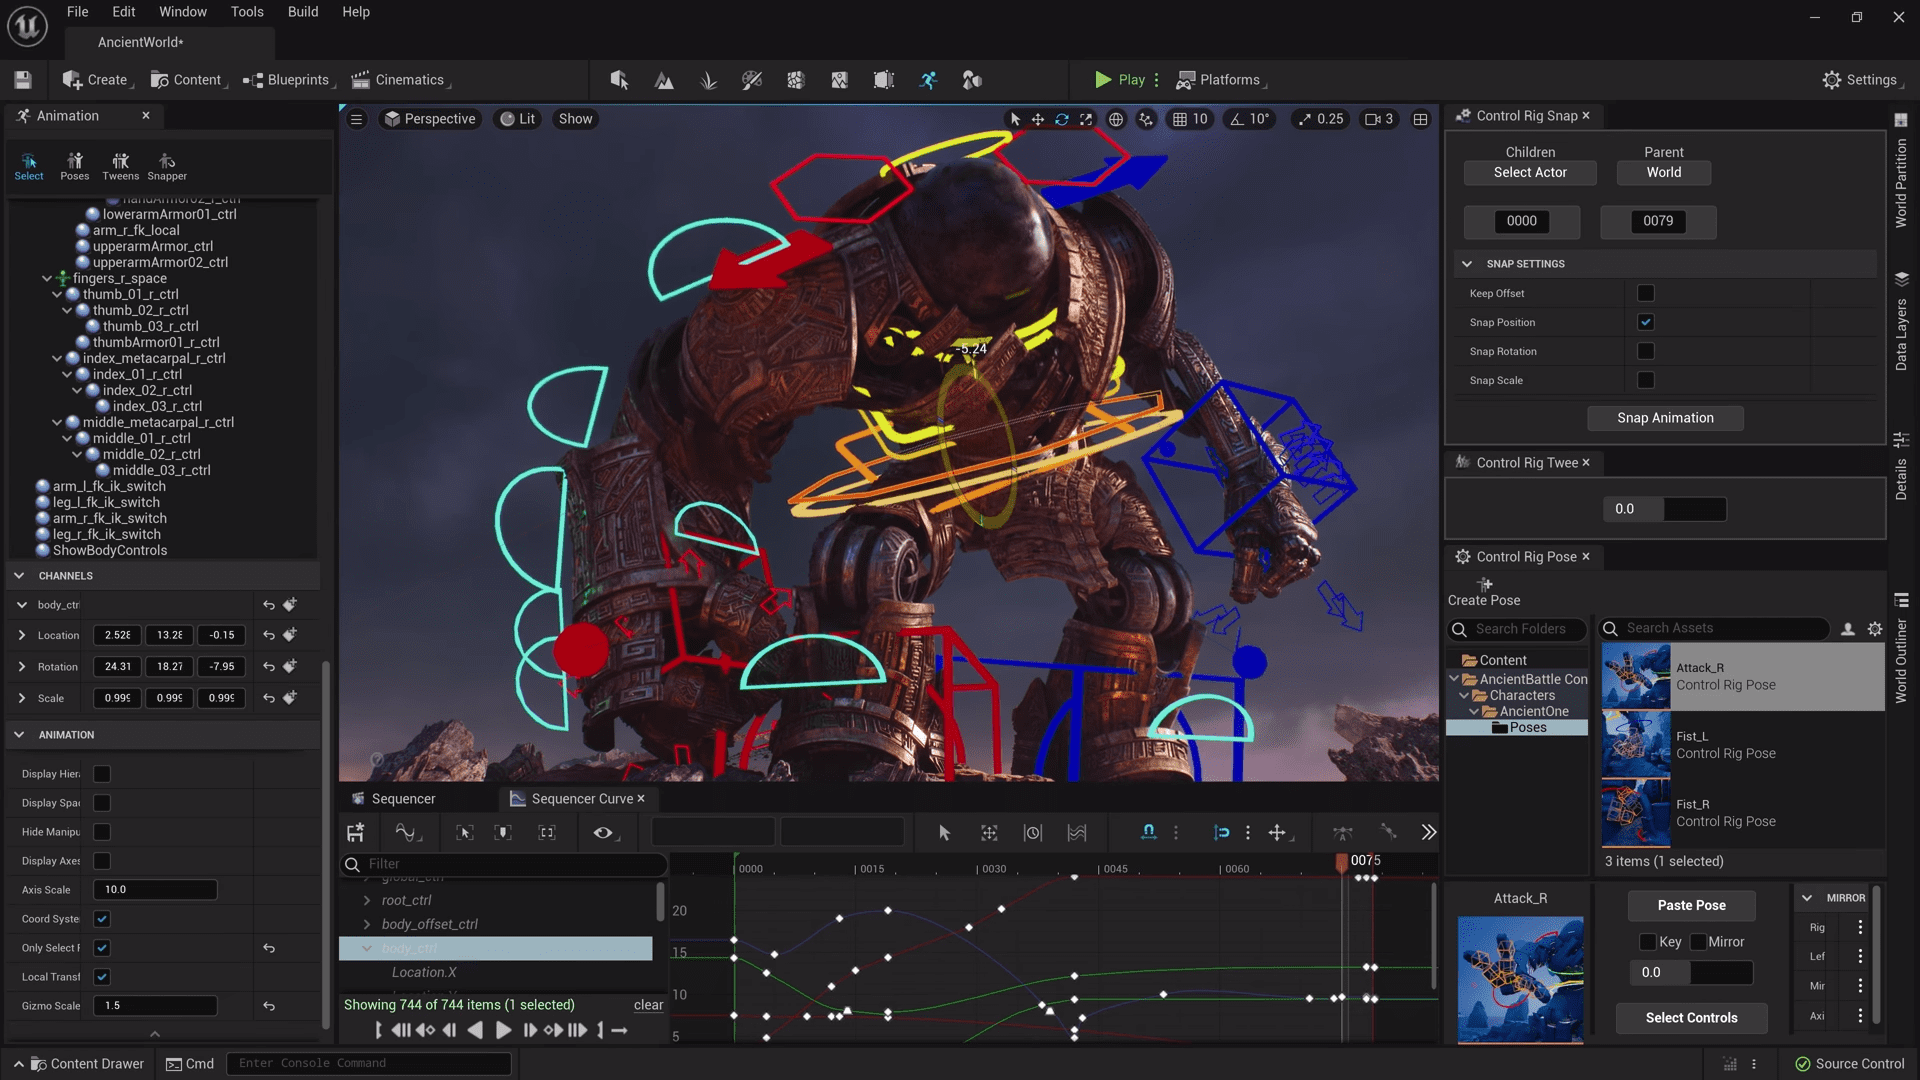
\includegraphics[width=1\textwidth]{img/unreal_engine_5.png}
\caption{Unreal Engine 5 \cite{unrealengine5}}
\label{fig:unrealengine5}
\end{figure}

Poskytuje používateľom rôzne mechanizmy, ktoré im umožňujú spustiť hru na rôznych platformách. Ďalej obsahuje rozsiahly systematický súbor nástrojov a editorov, ktoré pomáhajú používateľom manažovať a modifikovať ich objekty pri tvorbe umeleckých diel do hry. %EK: Poskytuju aku platformu?

Unreal Engine poskytuje výnimočnú grafickú kvalitu a neustále aktualizované rozhranie s novými nástrojmi a možnosťami, ktoré uľahčujú prácu s programovaním. Systém Blueprint, založený na uzlovom programovaní, umožňuje používateľom vytvárať akcie pre jednotlivé objekty bez nutnosti písania tradičného kódu. Tento tokovo-orientovaný prístup k programovaniu, známy ako low-code, umožňuje vývojárom efektívne vytvárať hry s možnosťou ďalšieho skriptovania a programovania v~jazyku C++. %PREROBENE

\subsubsection{Godot}

Popri mnohých herných enginoch na trhu, Godot je výborným herným enginom na vývoj low-cost hier a nie je tak populárny, ako Unity alebo Unreal. Avšak, po fiasku Unity s novou stratégiou monetizovania sa mnoho developerov začalo obzerať po alternatíve a Godot sa stal ich novým programovacím prostredím. Prvý krát sa objavil v~roku 2014, ako cross-platform herný engine orientovaný na 2D a 3D vývoj hier. Pre naše účely však neposkytuje takú škálu integrovaných AR knižníc, ako by sme potrebovali. Godot vznikol v~roku 2014, takže patrí určite medzi mladé herné enginy a programuje sa v~jazyku GDScript alebo ponúka aj podporu C++ \cite{zenva2023godot}. 

\begin{figure}[h]
\centering
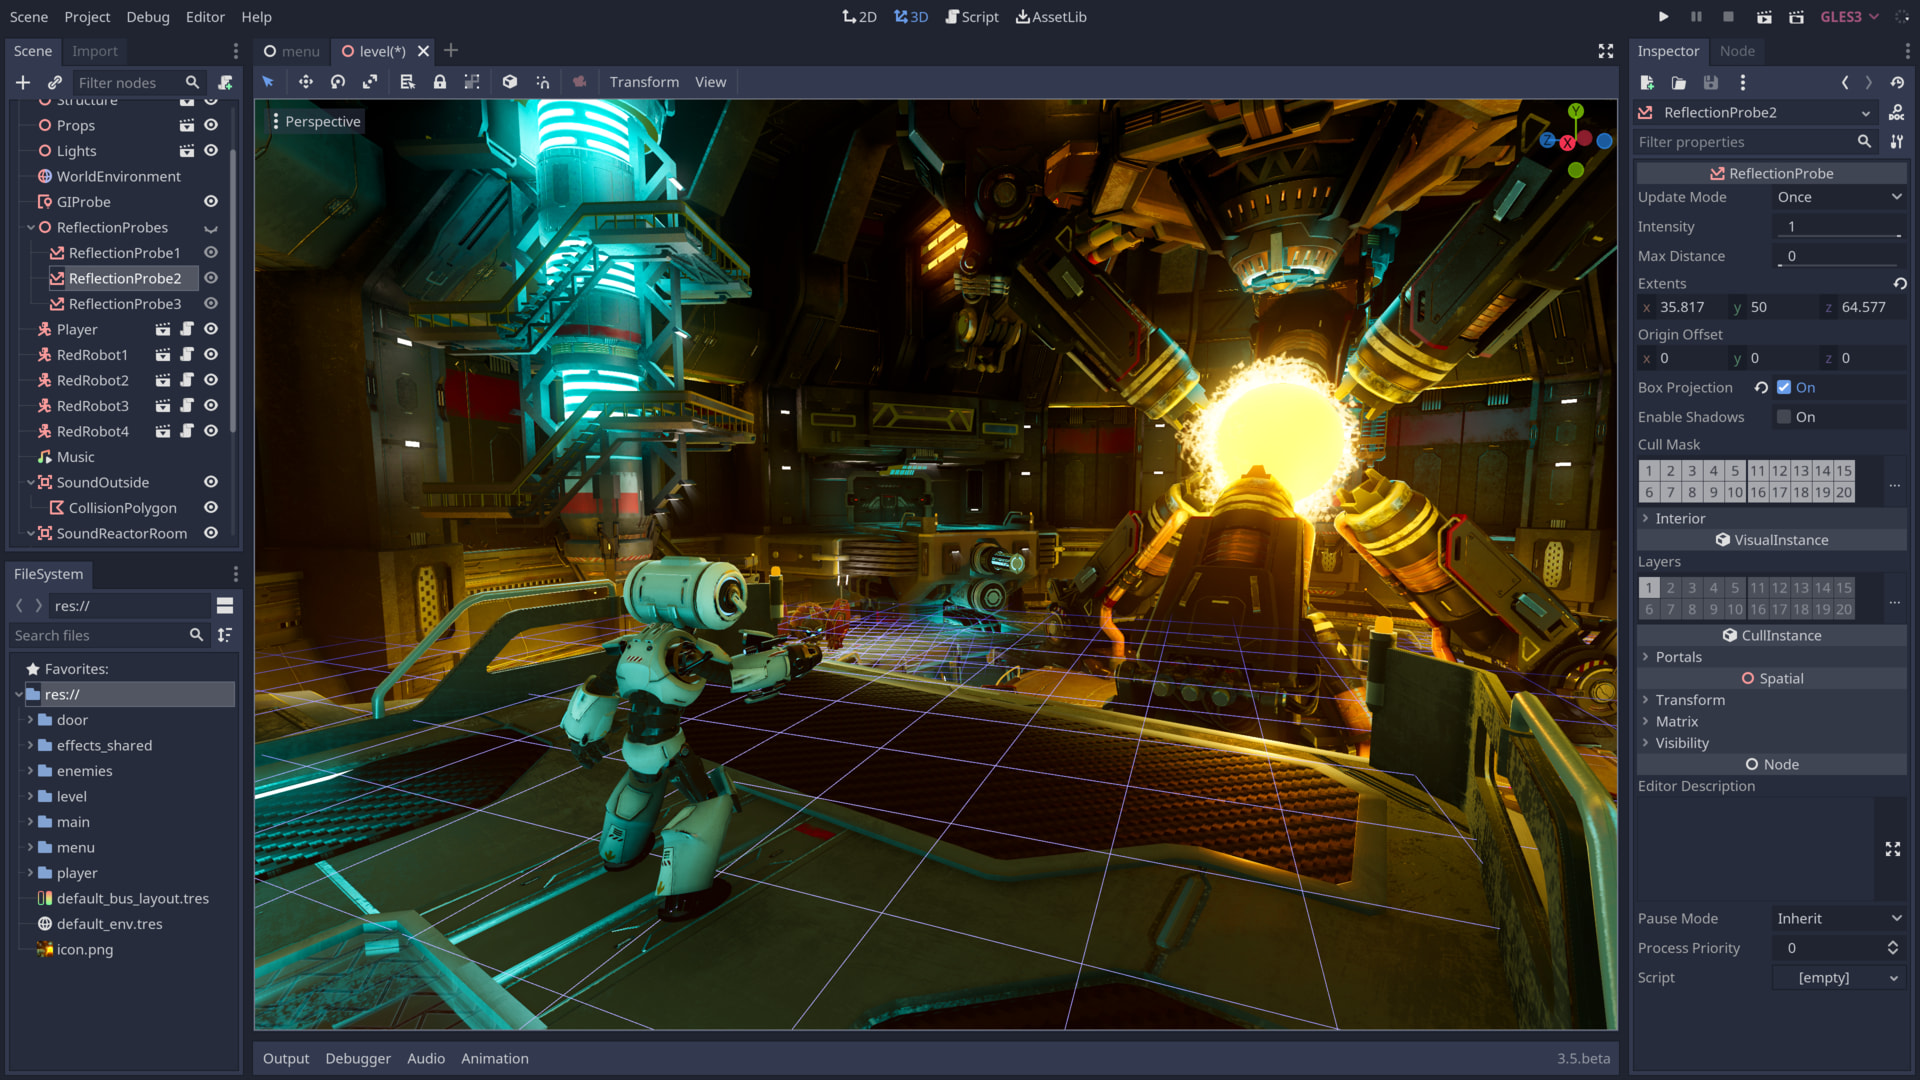
\includegraphics[width=1\textwidth]{img/godot_editor.jpg}
\caption{Godot \cite{godottps}}
\label{fig:godotEditor}
\end{figure}

\subsubsection{Unity}

Unity je herný engine pre takmer každého, keďže je pomerne jednoduché sa v~ňom naučiť pracovať a vyvíjať aplikácie, na to stačí základná orientácia v~tomto engine, pochopenie štruktúr class pri implementácii rôznych doplnkov a funkcií a schopný počítač na spustenie kompilácie a hry a chuť vytvárať nové veci alebo vylepšovanie už starých prostredníctvom kontribúcie do projektov napríklad na Githube.

Mnoho ľudí, ktorí sa aspoň trochu zaujímajú o hry, túžilo alebo stále túži vytvoriť svoju vlastnú hru. V~súčasnosti sa bariéry zvyšujú, a čas, investície a výkon sú veľmi žiadané, aj kvôli mobilným hrám. Jedným z~týchto engine-ov je Unity Engine. Nie je určený len pre malé vývojové štúdiá (alebo jednotlivcov); medzi mnohé herné tituly vytvorené v~Unity hernom engine patria napríklad Escape from Tarkov, Pokémon Go, Call of Duty Mobile, Cuphead, Cities: Skylines.%EK: opravit gramaticke chyby - opravene

Unity poskytuje široké množstvo nástrojov na vývoj mobilných hier a iných typov softvéru. Dokážeme implementovať aplikácie na škálu rôznych platforiem, ako je Windows, Android, iOS, Linux a macOS. 

\begin{figure}[h]
\centering
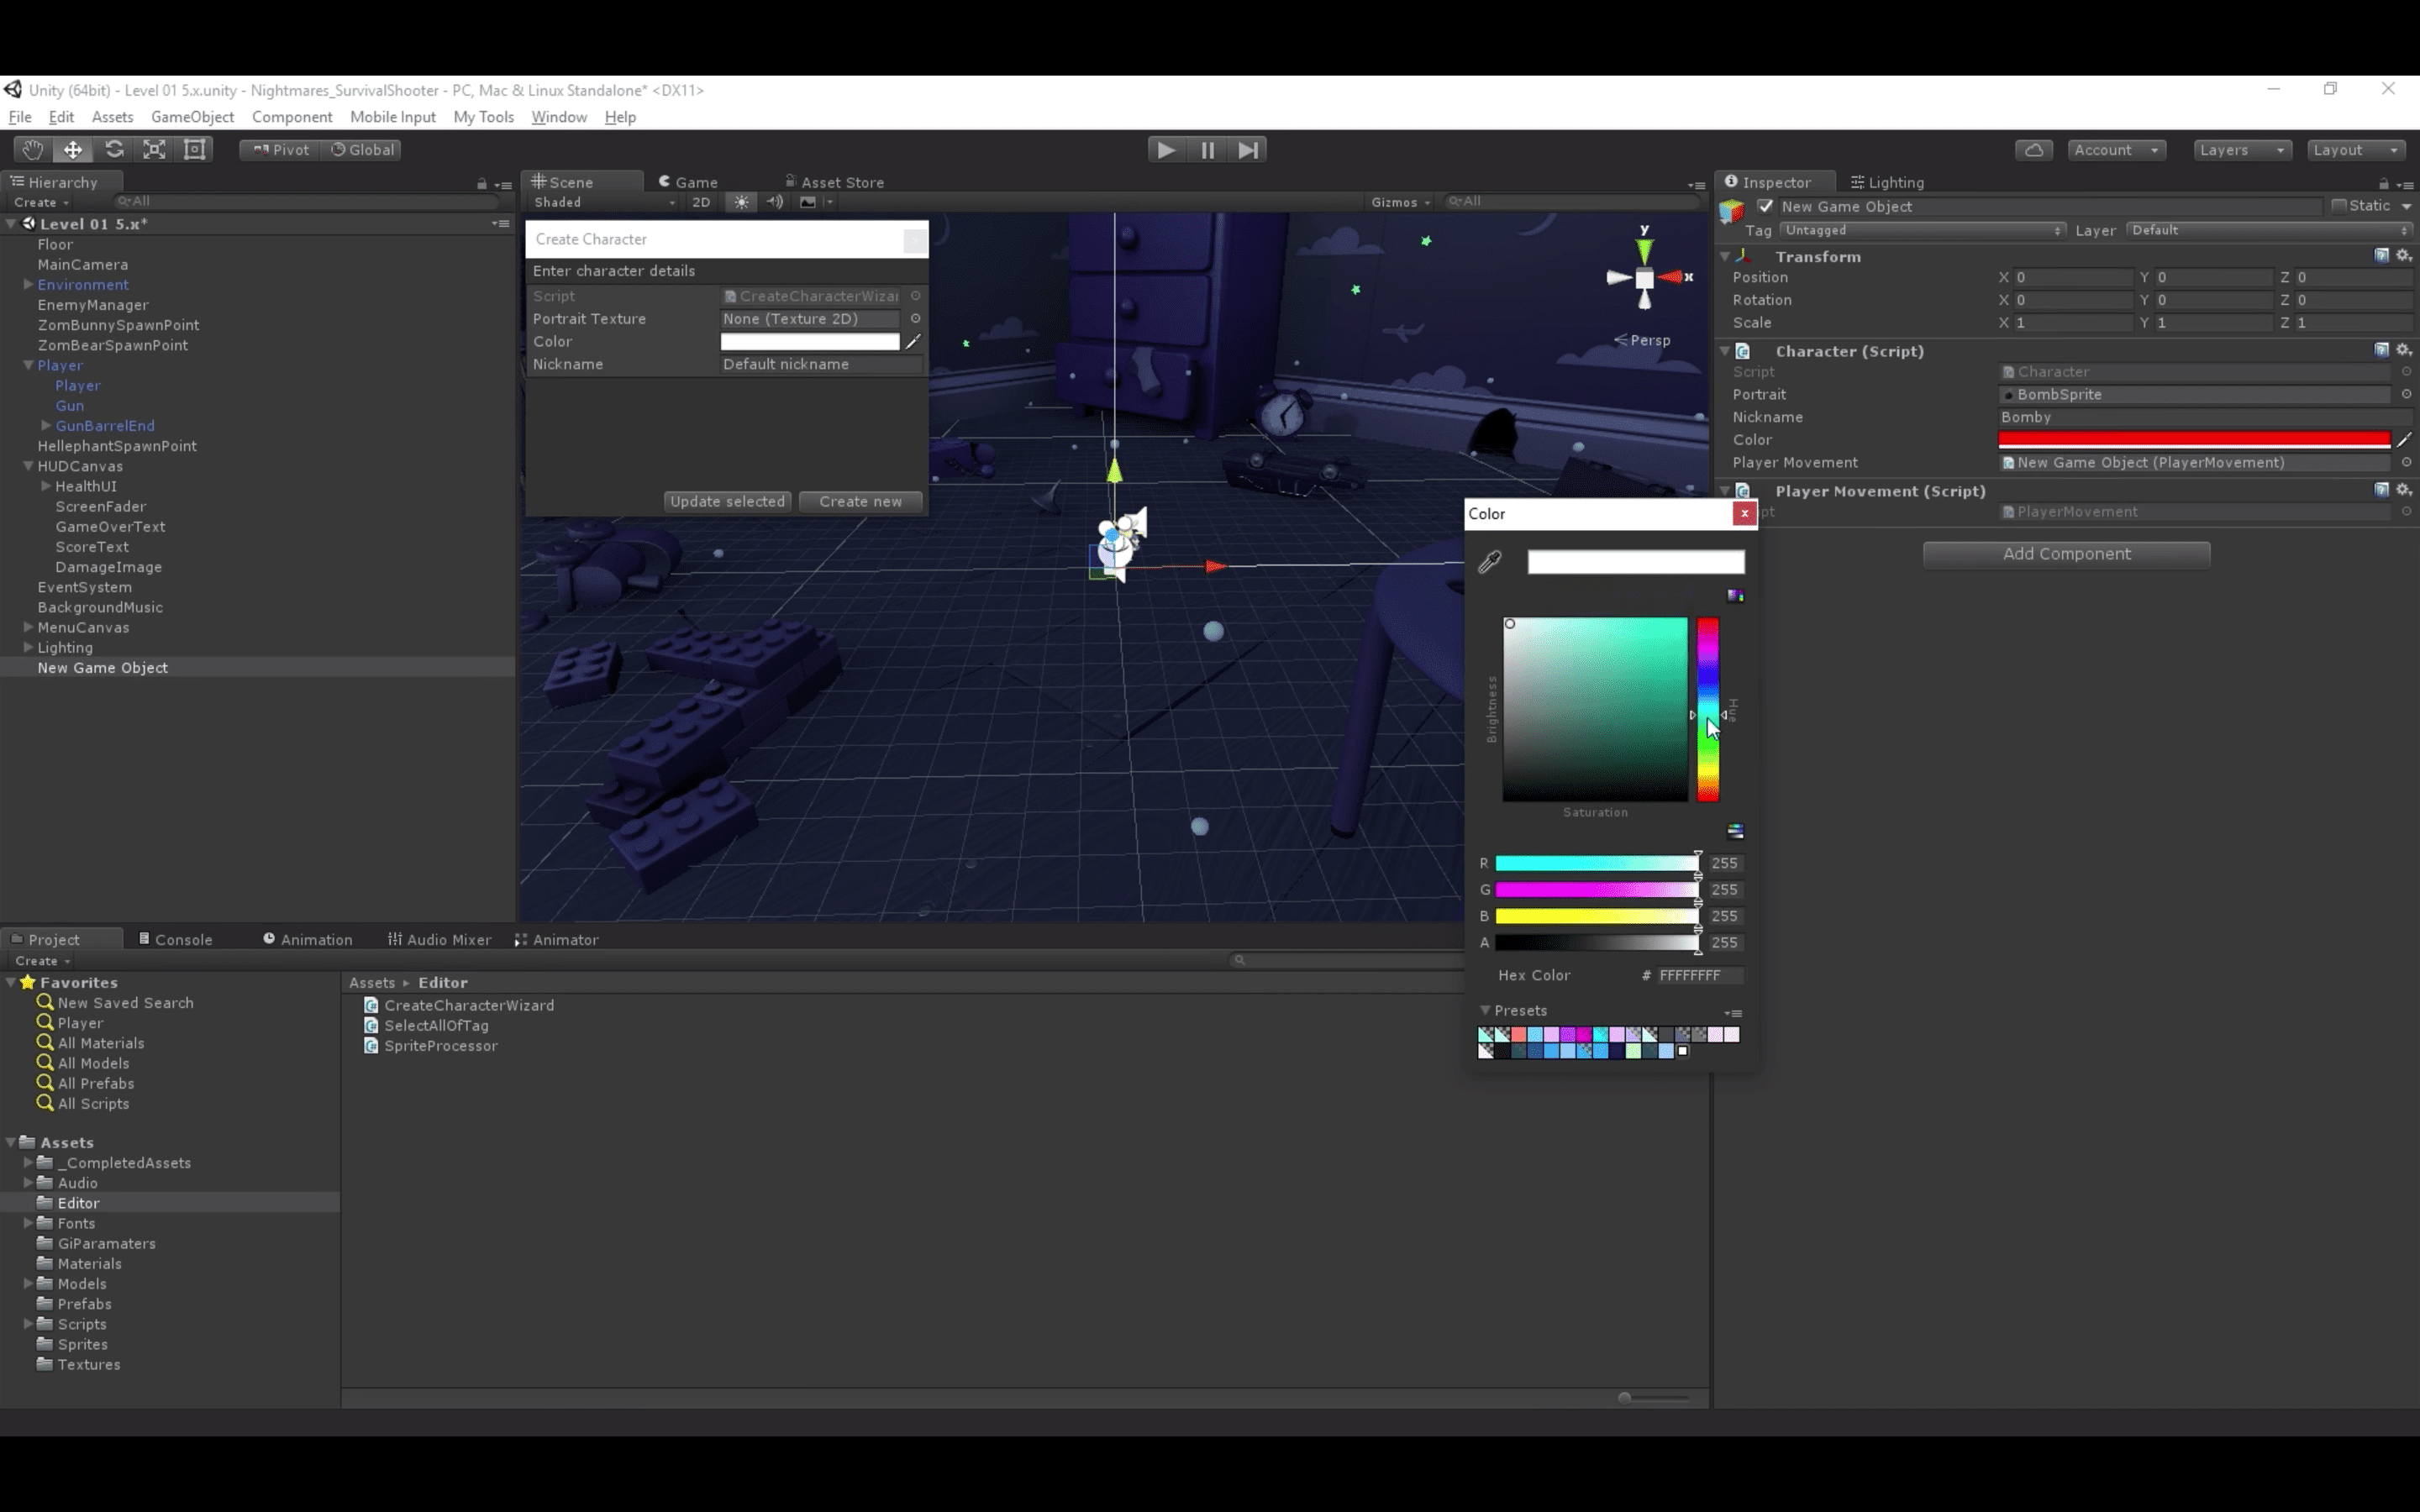
\includegraphics[width=1\textwidth]{img/unityEditor.png}
\caption{Unity \cite{unityscreenshot}}
\label{fig:godotEditor}
\end{figure}

Unity je založený na programovacom jazyku C\# a podporuje vytváranie 2D, 3D hier ale iných typov softvérových aplikácií pre oblasť priemyselu a služieb, ktoré vyžadujú 2D alebo 3D renderovanie v~reálnom čase. Štatistiky z roku 2022 ukazujú, že 70\% z top 1000 mobilných hier je vytvorených v~Unity hernom engine. K dnešnému dňu vygenerovalo Unity viac, ako 1.1 miliardy dolárov prostredníctvom reklám v~aplikáciach.

Engine funguje skrz assety, ktoré môžeme importovať alebo stiahnuť z Unity marketu, nachádza sa tam mnoho platených ale nájdu sa tam aj tie zadarmo. Unity taktiež poskytuje vývoj softvéru rozšírenej reality vďaka knižniciam kompatibilných s Unity, ktoré sme opisovali v~kapitolách vyššie. Taktiež Unity poskytuje obrovské množstvo tutoriálov priamo na ich stránke a taktiež je veľké množstvo materiálov o Unity prístupné zadarmo na internete, prípadne za platobnými bránami rôzne prémiové kurzy.

Pre prístup do Unity je možné si vybrať z rôznych typov subskripčných plánov. Medzi prvými je personálny, tento plán je zadarmo a poskytuje prístup do vývojovej platformy, do Unity Visual Scriptingu, Unity Version Control až do troch používateľov a rôzne ďalšie. Tento plán je sčasta dostačujúci pre každého začínajúceho aj pre malé herné štúdia. Plus stojí 399 dolárov za rok a Pro stojí približne 1800 dolárov na rok obsahujú ďalšie nástroje, ako je nasadenie aplikácií na konzoly, vývoj AR, support servis pre zákazníkov, a tak ďalej. Enterprise je prispôsobená kvóta, ktorú určuje Unity na základe zárobkov hry. 

Posledne taktiež existuje Industry plán, čo je typ predplatného, za okolo 4500 dolárov na rok, ktorý je primárne pre priemyselné podniky. Je vhodné podotknúť, že vzhľadom na nedávne udalosti sa Unity potýkalo s veľkou odozvou po vyhlásení novej monetizačnej stratégie, ktorá vrhla na Unity mnoho negativity \cite{lacoma2023unity}.%EK: Industry plan? Co to je? - PRIDANE čo je typ predplatného, za okolo 4500 dolárov na rok,

\begin{table}[!h]
\centering
\caption{Porovnanie herných enginov}
\label{tab:game-engines}
\begin{tabularx}{\textwidth}{|l|c|c|X|X|}
\hline
\textbf{Engine} & \textbf{Rok vydania} & \textbf{Jazyk} & \textbf{Typy hier} & \textbf{Hlavné atribúty} \\ \hline
Unreal Engine & 1998 & C++ & FPS, RPG, MMORPG & Blueprint, high-quality graphics \\ \hline
Godot & 2014 & GDScript/C++ & 2D and 3D games & Cross-platform, free and open-source \\ \hline
Unity & June 2005 & C\# & Mobile, PC games & Cross-platform, Unity Asset Store \\ \hline
\end{tabularx}
\end{table}

\FloatBarrier 

\subsubsection{Blender}

Blender 3D je open-source softvérová aplikácia, ktorá prináša silné a versatilné nástroje na vytváranie 3D modelov. Ponúka široké spektrum doplnkov a funkcií pre rôzne aspekty tvorby 3D, vrátanie modelovania, rigovania, animácií, simulácií, renderingu, kompozície a sledovanie pohybu. Je vyvíjaný firmou Blender Foundation a je dedikovaná komunite. Je to veľmi populárny nástroj, ktorý je známy, ako medzi začiatočníkmi, tak aj medzi profesionálmi v~3D kontentovom priemysle. 

Blender bol spočiatku vydaný firmou Blender Foundation v~roku 2002, ako zadarmo dostupné open-source softvérové riešenie. Jeho misia bola priniesť na svet najlepšiu 3D počítačovú grafickú technológiu na svete dostupnú pre umelcov a tvorcov. Po čase sa Blender vyvíjal a rástol, s priebežnými updatmi a vylepšeniami vďaka kolaboratívnemu úsiliu komunity. 

Práca v~nástroji Blender je pomerne jednoduchá na naučenie a obsahuje obrovské množstvo skratiek, ktoré uľahčujú tvorbu 3D modelov, avšak interface je veľmi komplexný a obsahuje veľké množstvo funkcií, že sa zo začiatku môže užívateľ cítiť preťažený. Obsahuje v~sebe množstvo nástrojov pri budovaní 3D a nie sú potrebné dodatočné nástroje, ako pri iných 3D modelovacích nástrojoch. 

Jednou z nevýhod je limitovaná integrácia s nástrojmi z tretej ruky, teda si nerozumie veľmi dobre s externými nástrojmi a pluginmi, ako iné komerčné značky. To sa však snaží kompenzovať budovaním vlastných knižníc a addonov, ktoré rozširujú jeho funkcionalitu \cite{hill2023blender}. 

\subsubsection{Cinema 4D}

Jedná sa o prostredie, ktorý slúži na profesionálne 3D modelovanie, animácie, simulácie a renderovanie. Poskytuje teda širokú škálu riešení pre užívateľov. Je to rýchly, silný, flexibilný a veľmi stabilný súbor nástrojov na vytváranie 3D workflowu s viac prístupnými a efektívnym prístupom pre dizajn, pohyblivú grafiku, VFX, AR/MR/VR, vývoj hier a všetky typy vizualizácií, ktoré môže profesionálny modelár potrebovať \cite{maxon2024cinema4d}. 

Jedná sa však o pomerné drahý nástroj, pre študentov je aktuálne nacenený na 73€ mesačne (kde má používateľ všetky produkty od firmy Maxon One), pre individuálnych používateľov na 84€ mesačne s balíkom kde sa nachádza len Cinema 4D \cite{maxon2024buy}. 

\subsection{Knižnice pre AR / MR}
Keďže sa rozšírená realita stáva čím ďalej tým viac populárnejšou, znamená to, že je potrebné vyrábať viac aplikácií, ktoré s ňou dokážu pracovať. Túto dieru na trhu začali vypĺňať rôzni technologickí giganti, ako je napríklad aj Google (ARCore) a Apple (ARKit) vlastnými knižnicami na vytváranie takýchto aplikácií. Na trhu je však aj mnoho iných knižníc, ktoré im dokážu konkurovať. Tými sú napríklad Vuforia, Wikitude a Visionlib. Tieto si predstavíme jednotlivo v~ďalších sekciách.

\begin{table}[h]
\centering
\caption{Porovnanie základných funkcií AR knižníc}
\label{tab:ar-features}
\begin{tabularx}{\textwidth}{|l|X|X|X|X|}
\hline
\textbf{AR knižnica} & \textbf{Sledovanie pohybu} & \textbf{Pochopenie prostredia} & \textbf{Odhad svetla} & \textbf{Podpora platforiem} \\ \hline
ARCore & Áno & Áno & Áno & Android, iOS \\ \hline
ARKit & Áno & Áno & Áno & iOS \\ \hline
Vuforia & Áno & Áno & Nie & Android, iOS, UWP, Unity \\ \hline
Wikitude & Áno & Áno & Nie & Android, iOS, HoloLens \\ \hline
VisionLib & Áno & Áno & Nie & Windows, Android, iOS \\ \hline
\end{tabularx}
\end{table}

\subsubsection{ARCore}

Arcore je platforma od Google určená na~vývoj aplikácií, ktoré využívajú rozšírenú realitu, čím poskytujú používateľom pútavý a interaktívny zážitok. Táto platforma využíva rôzne aplikačné programové rozhrania (API) na~integráciu digitálnych objektov do~reálneho sveta prostredníctvom fotoaparátu zariadenia. %PREROBENE

API je súbor pravidiel, protokolov a knižníc, ktoré umožňujú rôznym softvérovým programom komunikovať a integrovať medzi sebou. Jedná sa o rozhranie, ktoré poskytuje určité funkcie a možnosti pre iné programy, aby s~nimi mohli pracovať bez toho, aby museli poznať vnútornú štruktúru alebo detaily týchto funkcií. Využíva sa hlavne pri webových aplikáciach. Pričom web slúži, ako prostredník pre prácu s danou aplikáciou a API je implementovaný v~pozadí, ako Backend danej aplikácie. API ďalej pracuje s databázou, vykonáva rôzne výpočty, úpravu dát, implementáciu logiky atď \cite{kodouskova2020api}. 

ARCore povolí telefónu vnímanie prostredia a pochopenie sveta aby mohol následne interagovať s informáciami. Niektoré API sú dostupné skrz Android a iOS pre získanie AR skúseností. ARCore používa 3 kľúčové prvky na integrovanie virtuálneho kontentu s reálnym svetom, ktoré vníma skrz kameru. Tieto prvky sú:

\begin{itemize}
    \item \textbf{Motion tracking} alebo sledovanie pohybu umožňuje zariadeniu pochopiť a sledovať jeho pozíciu relatívne naprieč svetom.
    
    \item \textbf{Environmental understanding} alebo pochopenie okolia dovolí mobilnému telefónu detegovať veľkosť a polohu všetkých typov povrchov - horizontálne, vertikálne a sklonené povrchy, ako je napríklad zem, počítačový stôl alebo radiátor na stene či chladnička v~kuchyni.
    
    \item \textbf{Light estimation} alebo odhad osvetlenia umožňuje telefónu odhadnúť aktuálne svetelné podmienky prostredia.
\end{itemize}


ARCore je aktuálne navrhnutý pre prácu skrz rôznymi zariadeniami, ktoré majú integrovanú aspoň Android verziu 7.0 (Nougat) a novšie verzie \cite{google2024arcore}. 

ARCore nepotrebuje žiadne špeciálne senzory, keďže je to knižnica, ktorá je zameraná hlavne na mobilné telefóny, ktoré sú bežne dostupné pre každodenných konzumentov s bežnými kamerami. Inak povedané, nie sú potrebné žiadne vysoko úrovňové kamery používané na vedecké účely. (Existujú knižnice, ako je Project Tango, na túto knižnicu sú potrebné vysokoprofilové kamery a špeciálne senzory). To teda znamená, že sa spolieha len na kameru na mobilnom telefóne a senzor pohybu, ako je napríklad gyroskop, akcelerometer a komplikované softvérové triky implementované v~tejto knižnici. ARCore nasleduje sériu fundamentálnych konceptov aby dokázala táto knižnica úspešne interpetovať čo kamera vidí a na základe týchto informácií poskytuje užívateľovi integrovaný zážitok s rozšírenej reality \cite{conway2023arcore}. 

ARCore knižnica využíva  simultánne lokalizovanie a mapovanie (simultaneous localization and mapping), alebo inak povedané \gls{slam}, na chápanie kde presne sa mobilný telefón nachádza vzhľadom na svet okolo neho. Dokáže vypočítať zmeny v~polohe detegovaním vizuálne rozdielnych prvkov zachytených na kamerovom zázname a potom to použiť, ako zachytávacie body, podľa toho vie či sa zmenila poloha a jednotlivé charakteristické znaky danej lokácie. Využíva teda tieto charakteristické znaky na zachytávanie plôch alebo horizontálnych, prípadne vertikálnych povrchov a používa ich pre vytvorenie dodatočného kontextu. 

Pre odvodenie polohy kamery (poloha a orientácia) vzhľadom na prostredie v~čase sa páruje dodatočne s inerciálnymi meraniami z IMU zariadenia (Inertial Measurement Unit) \cite{conway2023arcore}. 

\gls{imu} je zariadenie alebo senzor, ktorý meria zrýchlenie a uhly rotácie (gyroskopické hodnoty) v~troch rôznych osiach \cite{vectornav2024imu}.

Používaním týchto informácií a kontextu môže vývojár renderovať veci na kamerovom zázname a spraviť to tak, že to vyzerá, ako keby to bolo súčasťou reálneho sveta. Taktiež dokáže ovplyvniť koľko svetla sa na ploche nachádza a používaním tohoto kontextu môže renderovať obrázok, ktorý vyzerá svetlejšie alebo tmavšie na základe toho koľko svetla sa zachytáva v~kamere. Ako výsledok je teda realistickejšie zobrazenie umelo pridaného objektu.

Tieto fundamentálne koncepty sú len povrchovo zhrnuté, v~pozadí sa odohrávajú veľmi komplikované výpočty a často využívajú rôzne fyzikálne zákony, ktoré následne program prepočítava do výsledku, ktorý môžeme vidieť na zázname z kamery.

Jednou zo zaujímavých doplnkov Google ARCore je taktiež Cloud Anchors, to dovoľuje položiť, ktorý je viditeľný v~rámci Cloudovej relácií a aj iný používatelia, ktorí sa napoja na túto reláciu môžu vidieť tento objekt na tom istom mieste \cite{conway2023arcore}. 

\subsubsection{ARKit}

ARKit je knižnica vytvorená firmou Apple a využíva iOS zariadenia. Dovoľuje, rovnako, ako ARCore, developerom produkovať aplikácie, ktoré umožňujú interakciu so svetom využívaním kamery a senzorov. 

Apple videl veľké využitie AR v~budúcnosti mobilných telefónov, preto sa rozhodli vyplniť dieru na trhu a vytvoriť si vlastnú knižnicu, vďaka ktorej by mohli poskytnúť developerom vhodnú knižnicu na vytváranie AR aplikácií. Túto knižnicu predstavili v~oku 2017, ako súčasť iOS 11. Taktiež zároveň oznámili ďalšiu verziu v~iOS 12 a v~podstate vydávajú novu verziu ARKit vždy keď vyjde nova verzia iOS. 

Má veľmi veľa podobných prvkov, ako ARCore, preto nemusíme znovu vysvetľovať jednotlivé koncepty, ako AR funguje. Pozrieme sa však na podstatné rozdiely oproti ARCore.

ARKit využíva technológiu zvanú Visual Inertial Odometry (VIO) na sledovanie sveta okolo iPadu alebo iPhonu, to im dovoľuje vnímať, ako sa pohybuje mobilný telefón priestorom. ARKit využíva tieto dáta nielen na analýzu rozpoloženia izby alebo priestoru, ale taktiež deteguje horizontálne plochy, ako je stôl alebo podlaha. Následne vďaka tomu môžeme položiť objekt na tieto plochy rovnako, ako pri ARCore, ak to je vec ktorú chceme dosiahnuť využívaním takejto aplikácie.

Predpoklady pre vývoj tejto knižnice sú, že v~budúcnosti bude môcť človek využívať rozšírenú realitu aj v~rámci toho, že bude mať okuliare, predstavme si teda Apple AR okuliare, ktoré následne môžu rozširovať našu realitu nosením takéhoto zariadenia, nie len teda snímaním kamery a využívaním konkrétnej aplikácie.

ARKit a Google ARCore poskytujú funkcionalitu Cloud Anchors, ktorá umožňuje zdieľanie virtuálne umiestnených objektov v~rámci viacerých zariadení. Keď sa k takejto AR relácii pripojí druhé zariadenie, môže vidieť tú istú scénu rozšírenej reality. Táto technológia tiež umožňuje pozastaviť a neskôr znovu spustiť reláciu, čo uľahčuje návrat používateľov do virtuálnej scény. Ako príklad, si predstavte predizajnovanie obývačky: Užívatelia môžu v~obývačke virtuálne umiestniť napríklad skriňu. Tento objekt sa zobrazí aj na iných zariadeniach, ktoré sú súčasťou relácie. Ak sa k scéne vrátia, napríklad o deň neskôr, a znovu naskenujú obývačku, uvidia skriňu na tom istom mieste a môžu ju premiestniť alebo pridať ďalšie prvky. %PREROBENE

\begin{table}[h]
\centering
\caption{Podrobné porovnanie funkcií medzi ARCore a ARKit}
\label{tab:arcore-arkit-comparison}
\begin{tabular}{|l|c|c|}
\hline
\textbf{Funkcia} & \textbf{ARCore} & \textbf{ARKit} \\ \hline
Sledovanie pohybu & Áno & Áno \\ \hline
Pochopenie prostredia & Áno & Áno \\ \hline
Odhad svetla (Light estimation) & Áno & Áno \\ \hline
Visual Inertial Odometry & Nie & Áno \\ \hline
Cloud Anchors & Áno & Áno (s podobnou funkcionalitou) \\ \hline
Multiplatformová podpora & Áno (Android, iOS) & Nie (iba iOS) \\ \hline
Sledovanie tváre & Nie & Áno \\ \hline
3D objektové sledovanie & Áno & Áno \\ \hline
\end{tabular}
\end{table}

\subsubsection{Vuforia}

Vuforia je multi-platformová knižnica pre Zmiešanú realitu (MR) a rozšírenú realitu (AR) s plným trackovaním a implementáciou na rôznych typoch hardvéroch vrátane mobilných zariadení a HMD, ako je Microsoft HoloLens. %PREROBENE

Vuforia je platforma pre vývoj aplikácií rozšírenej reality, ktorá je dostupná buď ako samostatný softvér alebo ako knižnica integrovateľná s vývojovým prostredím Unity. Táto integrácia umožňuje vytváranie vizuálnych aplikácií a hier pre Android a iOS s využitím jednoduchého drag-and-drop (ťahaj a pusti) workflow, čo zjednodušuje prácu vývojárov. %PREROBENE

Hlavné výhody Vuforie zahŕňajú podporu operačných systémov Android, iOS a UWP, ako aj podporu v~Unity Editor. Ďalším kľúčovým prvkom je PTC development toolkit, ktorý umožňuje sledovanie a rozpoznávanie špecifických obrázkov, modelov, objektov alebo 3D scanov. Táto funkčnosť je veľmi užitočná pre tvorbu interaktívnych a vizuálne atraktívnych aplikácií rozšírenej reality. %PREROBENE

%od tadeto neskontrolovane _____________________________________________________________________________________________

Aplikácie Vuforie môžeme spúšťať na iOS aj Android zariadeniach a dokonca aj na starších iPhone modeloch, ktoré nepodporujú ARKit. Ak dané zariadenie podporuje ARKit alebo ARCore, Vuforia ich využíva; v~opačnom prípade sa spolieha na vlastnú platformu.

Jadrom vývoja pomocou Vuforie je hlavne sledovanie obrazu a objektov. Vuforia podporuje nahrávanie modelov, obrázkov, scanov objektov a iných typov cieľov pre detekciu. Týmto môžeme nahrávať detekciu objektov zo špecifikovaných cieľov pre rozpoznávanie.

Tento nástroj pomáha pri identifikácií s rôznymi kategóriami, ako sú krabice, cylindre a plochy. Taktiež rozpoznáva text a prostredie. VuMark je hybridný typ fotky a QR kód, je to iný nápomocný doplnok, ktorý Vuforia poskytuje. Vuforia Object Scanner umožňuje vývojárom skenovať a vytvárať cieľové objekty. 

Krátke vysvetlenie jednotlivých doplnkov Vuforie:

\begin{itemize}
    \item \textbf{Model Targets} - Modelové ciele - používajú 3D model na rozpoznávanie predmetov, ktorých základom je ich samotná forma. Môžeme nainštalovať AR kontent na viacerých objektoch z rôznych uhlov na veľkom rozsahu produktov, ako je industriálna výroba, autá a hračky.
    
    \item \textbf{Image Targets} - Obrazové ciele - obrázky sú najjednoduchším spôsobom, ako pozmeniť reálne materiály na rovné povrchy, ako sú napríklad stránky magazínu, iné obrazy alebo zberateľské kartičky.
    
    \item \textbf{Multi Targets} - Multiciele - používa sa na objekty s viacerými hranami a rovnými povrchmi alebo zahŕňajú viaceré obrázky. Multiciele zahŕňajú obaly produktov, plagáty a maľby.
    
    \item \textbf{Cylinder Targets} - Cylinderové ciele -  Môžeme použiť cylindrové ciele pre umiestnenie AR informácie na cylindrické alebo kužeľové objekty. Sú ideálne na plechovky od sódy, fľaše a tuby s vytlačenou grafikou.
    
    \item \textbf{Object Targets} - Objektové ciele - Skenovanie objektu produkuje objektové ciele. Sú excelentným výberom pre hračky a iné predmety s konzistentnou formou a bohatými povrchovými detailami. 
    
    \item \textbf{VuMarks} - Môžeme použiť VuMarks na identifikáciu a pridávanie kontentu na skupinku objektov. Je to excelentná metóda na doplnenie produktových liniek, inventáre a stroje s informáciami a kontentom. 
\end{itemize}

\cite{anand2024vuforia}

\subsubsection{Wikitude}

Wikitude SDK pre Unity je plugin pre Unity3D, ktorý pridáva funkcionalitu rozšírenej reality do Unity prostredia. Je optimalizované na detekciu a sledovanie obrazov a objektov v~rámci zážitkov rozšírenej reality. Môže sa používať spolu s natívnymi AR frameworkmi, ako sú ARCore, ARKit a HoloLens, alebo cez wrappery, ako je AR Foundation. Alternatívne môže fungovať aj, ako samostatný nástroj na poskytovanie AR zážitkov.

\begin{itemize}
    \item Používaním Wikitude \gls{sdk} pre Unity môžeme využívať tieto vlastnosti knižnice:
    \begin{itemize}
        \item Sledovanie obrazov na zariadení
        \item Sledovanie cylindrických objektov
        \item Sledovanie obrazov z cloudového servera
        \item Sledovanie viacerých obrazov súčasne
        \item Sledovanie objektov a scén
        \item Sledovanie viacerých objektov súčasne
        \item Kombinovanie viacerých trackerov z vyššie uvedených v~jednej relácií AR
    \end{itemize}
    \item Môžeme využívať všetky uvedené naraz v~kombinácií s pozičným sledovaním pomocou ARCore, ARKit a AR Foundation
\end{itemize}

Wikitude SDK knižnica pre Unity je rozšírením funkcionalít ARKit knižnice a ARCore knižnice doplnkami, ktoré niesu prítomné v~natívnych verziách týchto AR frameworkov alebo prichádza s inými kvalitatívnymi štandardami v~porovnaní s implementáciou vo Wikitude SDK. V~tomto smere, Wikitude SDK môžeme vidieť, ako rozšírením ARkit knižnice a ARCore knižnice. Používanie týchto (ARCore knižnice a ARKit knižnice) nie je povinné pre používanie Wikitude SDK.

Wikitude SDK môže využívať AR Foundation od Unity alebo fungovať úplne samostatne. Keďže AR Foundation je skvelým wrapperom ARCore knižnice a ARKit knižnice a iných AR frameworkov, neprináša žiadne funkcionality navyše \cite{wikitude2023sdk}. 

\subsubsection{VisionLib}

VisionLib umožňuje vývojárom tvoriť aplikácie rozšírenej reality s pokročilým trackovaním počítačového videnia pre priemyselné použitie. Táto knižnica využíva takzvaný Enhanced Model Tracking. VisionLib je široko uznávaná ako jedna z popredných knižníc pre trackovanie v~rozšírenej realite v~priemyselných aplikáciách. V každej aplikácii rozšírenej reality sú kľúčové počítačové videnie a trackovanie modelov, ktoré umožňujú obohatiť fyzické objekty o digitálne informácie. Či už na opravu a údržbu, AR založenými tréningovými kurzami, marketingové alebo predajné ciele, nič z týchto by nefungovalo, bez precízneho a spoľahlivého objektového detegovania a sledovania.

VisionLib je teda multi-platforomová AR trackovacia knižnica, ktorá integruje celú škálu algoritmov potrebných na sledovanie cieľov v~rozšírenej realite.  

S VisionLib môžete vytvoriť aplikácie v~Unity3D a nasadiť ich na Windows(32-bit aj 64-bit), Android (arm7, Android 4.4+) a iOS zariadenia. Taktiež môžete integrovať aplikáciu aj na iné operačné systémy používaním kódu v~čistom programovacom jazyku C. Dodatočne poskytuje simplifikovaný objective-C interface, ktorý dovoľuje používanie SDK na programovanie natívnych macOS a iOS aplikácií. 

Jadro SDK sa skladá z dynamických a statických knižníc, ktoré môžeme pripnúť k aplikácií. Aktuálne API ponúka čistú a zostrihaný prístup do funkcionality jadra enginu. Je to teda multi-platformová, na širokú škálu zariadení používateľná knižnica podporujúca vývoj v~Unity3D a taktiež na týchto natívnych platformách, ako je iOS, Android, UWP, macOS a Windows. Čo sa týka zariadení podporuje desktopové zariadenia, tablety, smartfóny a smart okuliare. 

Trackerovací systém v~VisionLib umožňuje kontinuálne sledovanie lokálne, bez nutnosti internetového pripojenia alebo pripojenia k online službám VisionLib.

Základné sledovacie správania v~VisionLib je možné riadiť pomocou konfiguračných súborov so špecifickou koncovkou '.vl', napríklad TrackingConfigurationFile.vl. Developeri môžu nastaviť metódu sledovania, ovplyvniť centrálne sledovacie parametre, definovať, ktorá kamera sa používa na sledovanie na zariadení s viac kamerami, definovať list modelov pri sledovaní viacerých modelov naraz, prepojiť rôzne vstupné zdroje, ktoré budú používané alebo nastaviť debug parametre počas vývoja aplikácie. Tieto konfiguračné súbory sú v~podstate JSON súbory s presne danou štruktúrou.

Niektoré takéto konfiguračné parametre môžu slúžiť aj, ako deklaratívne príkazy, ktoré môžeme napríklad použivať vnútri Unity GUI systéme na kontrolovanie alebo spúšťanie jednotlivých doplnkov a nakonfigurovať ich tam. Pre zhrnutie sú teda tieto konfiguračné súbory veľmi rýchlo deklarovateľným spôsobom, ako delegovať a ovládať správanie VisionLib a ovplyvniť sledovacie výsledky bez komplikovaného písania kódu. 

Avšak ak chceme používať VisionLib je potrebné mať licenčný súbor, bez neho nie je možné používať VisionLib a taktiež ani testovať aplikáciu. Po registrácií je potrebne tento súbor stiahnuť a vložiť do priečinku v~Unity. \cite{visionlib2023docs}

\subsection{S akým \gls{hw} sa pracuje}

Našu aplikáciu implementujeme hlavne na systémy Android, Unity umožňuje spustenie aplikácie priamo v~Unity, preto sme často testovali s web kamerou z notebooku alebo z externej web kamery. Avšak Vuforia nedovoľuje export aplikácie na Windows, preto cieľovým zariadením je Android. Taktiež je oveľa praktickejšie snímanie objektov s menším zariadením, ako je telefón alebo tablet. Finálne testovanie sme uskutočňovali pomocou tabletu Galaxy Tab S8 s modelom SM-X700. Tento tablet má duálnu kameru s 13 MP, f/2.0, 26mm (wide), 1/3.4", 1.0µm, AF
6 MP, f/2.2, (ultrawide) parametrami.

\section{Ciele práce}

\subsection{Stav riešenia problematiky na FEI STU}

Na Fakulte elektrotechniky a informatiky Slovenskej technickej univerzity (FEI STU) sa realizuje viacero projektov zameraných na vývoj a implementáciu nových technológií v~oblasti rozšírenej a zmiešanej reality. Tieto projekty sa sústreďujú na inovatívne metódy identifikácie a rozlišovania objektov v~priemyselnom a logistickom prostredí pomocou 3D identifikátorov.

Na Ústave automobilovej mechatroniky FEI SU sa výskumné aktivity zameriavajú ah na programatické generovanie 3D identifikátorov pre rozlišovanie zhodných entít v~prostredí zmiešanej reality. Hlavným cieľom je vývoj algoritmov pre generatívne modelovanie, ktoré by boli aplikované v~praxi priamo v~priemyselných podnikoch a logistických reťazcoch. Tento prístup by mohol nahradiť konvenčné metódy identifikácie, ako sú 2D čiarové kódy, a umožniť rozpoznávanie objektov z ľubovoľného uhla a z väčšej vzdialenosti.

Výskum sa zaoberá návrhom originálnych 3D identifikátorov pre aplikácie rozšírenej reality, ktoré budú vytvárané pomocou techník generatívneho modelovania a aditívnej výroby (3D tlače). Tento projekt sa snaží riešiť niektoré obmedzenia konvenčných identifikačných metód, ako sú nedostatky pri interakcii s objektami v~rôznych rovinách a prostredí s horšou viditeľnosťou.

Výskumné aktivity majú silné prepojenie s priemyselným partnerom, ktorý sa zameriava na využitie rozšírenej reality v~e-commerce. Spolupráca s priemyslom zabezpečuje, že výsledky výskumu majú priamy dopad na zlepšenie procesov a zefektívnenie práce v~priemyselných a logistických systémoch.

FEI STU aktívne podporuje integráciu týchto nových technológií do vyučovacích osnov a vedeckých aktivít. Výsledky projektov sú publikované v~prestížnych medzinárodných časopisoch a sú chránené patentmi a úžitkovými vzormi, čo značí vysokú úroveň inovácií a vedeckého prínosu univerzity.

Pokračujúci vývoj v~oblasti 3D identifikátorov a rozšírenej / zmiešanej reality na FEI STU ukazuje sľubné perspektívy pre ďalšie výskumné a aplikované projekty. Tieto technológie sa stávajú kľúčovými nielen v~akademickom prostredí, tak aj v~komerčnom nasadení. Týmto spôsobom FEI STU nielenže prispieva k teoretickému poznaniu, ale aj k praktickej aplikácii nových technológií.

%\subsubsection{Záver a perspektívy pre budúci vývoj}

%Projekty, ako PROG3D a 3D-IDENT-MR sú príkladom, ako FEI STU vyvíja strategické partnerstvá s priemyselnými subjektmi, ako je SmartBase s. r. o., čo vedie k priamej aplikácii výsledkov výskumu v~praxi. Tieto partnerstvá pomáhajú premostiť medzeru medzi akademickým výskumom a priemyselnými potrebami, čím sa zvyšuje relevancia výskumu a jeho dopad na spoločnosť. Zároveň poskytujú platformu pre študentov a mladých výskumníkov na získanie hodnotných skúseností v~reálnych priemyselných aplikáciách.

%Ústavy, ako ÚAMT, ÚIM a ÚEF sú strediskami inovácií na FEI STU, ktoré kontinuálne vyvíjajú nové metódy a technológie v~oblastiach, ako kyberneticko-fyzikálne systémy, rozšírená realita a 3D modelovanie. Tieto technológie sú základom pre budúci vývoj v~digitálnej transformácii, ktorá je kľúčová pre Industry 4.0 a ďalšie pokročilé priemyselné aplikácie.

%Celkovým cieľom FEI STU je nielen pokračovať v~prieskume na hrane možného v~oblasti rozšírenej reality a 3D identifikácie, ale aj udržať vedenie v~týchto technológiách na Slovensku a v~medzinárodnom kontexte. Výsledky a inovácie generované týmito projektmi posilňujú pozíciu univerzity, ako lídra v~technologickej inovácii a aplikácii nových riešení, čo priamo prispieva k rozvoju technického vzdelávania a výskumu v~Európe.

\subsubsection{Zhrnutie}

Výskumné aktivity na FEI STU ilustrujú dynamický prístup k riešeniu súčasných výziev v~priemysle a logistike prostredníctvom pokročilých technológií rozšírenej reality a 3D identifikácie. Uvedené projekty a spolupráce naznačujú silnú orientáciu na inovácie a praktické aplikácie, čo umožňuje FEI STU ostať v~popredí technologického vývoja a vzdelávania.

{\large\textbf{Čo riešime našou prácou}}

V súčasnosti sa priemyselné podniky usilujú o zavádzanie moderných technológií na ovládanie a diagnostiku zariadení, ktoré využívajú vo svojej prevádzke. Jedným z najnovších trendov je využitie virtuálnej a rozšírenej reality. Tieto technológie umožňujú pracovníkom lepšie interagovať s priemyselným zariadením a efektívnejšie riešiť problémy.

Hlavným cieľom nášho projektu je vyvinúť spôsob, ako jednoducho a efektívne identifikovať rôzne zariadenia v~rozšírenej realite. Na dosiahnutie tohto cieľa plánujeme vytvoriť prototypy 3D identifikátorov, ktoré budú navrhnuté a vytlačené pomocou 3D tlačiarne. Tieto identifikátory nám umožnia okamžite rozpoznať a zobraziť dôležité informácie o zariadeniach pri pohľade cez zariadenia zmiešanej reality, ako sú napríklad smart okuliare.

Tento prístup nie len zvýši efektivitu a presnosť pri práci s priemyselnými zariadeniami, ale tiež zlepší bezpečnosť pracovníkov tým, že im poskytne potrebné informácie priamo v~ich zornom poli, bez potreby fyzického prezerania manuálov alebo dotykových panelov. S našim riešením sa zariadenia stanú inteligentnejšími a ich obsluha intuitívnejšia a rýchlejšia.

%DOPLNENE

\subsection{Vytýčenie cieľov diplomovej práce}
V tejto časti sú predstavené hlavné ciele diplomovej práce, ktoré sa zameriavajú na vývoj a porovnanie technológií a metodík v~oblasti rozpoznávania 3D objektov v~prostredí zmiešanej reality. Ciele sú rozdelené do štyroch základných oblastí:

\subsubsection{Štúdium a porovnanie existujúcich metód rozpoznávania 3D objektov}
Cieľom je naštudovať a porovnať rôzne postupy rozpoznávania 3D objektov používané v~súčasných softvéroch pre zmiešanú realitu. Analýza zahŕňa prehľad softvérových platforiem, ako sú ARKit od Apple, Wikitude, VisionLib, Vuforia, ARCore od Google a Microsoft HoloLens. Štúdium sa zameria na porovnanie ich prístupov, algoritmov a účinnosti v~rôznych scenároch použitia.

\subsubsection{Návrh metodiky rozpoznávania 3D identifikátorov}
Druhým cieľom je navrhnúť metodiku rozpoznávania 3D identifikátorov, ktoré by mohli byť využité pri zabezpečovaní ovládania a monitorovania zariadení s využitím rozšírenej alebo zmiešanej reality. Tento návrh by mal obsahovať výber vhodnej knižnice pre rozšírenú realitu, definovanie typov 3D identifikátorov a vývoj algoritmov pre ich detekciu a rozpoznávanie.

\subsubsection{Implementácia a testovanie programu pre rozpoznávanie 3D identifikátorov}
Tretí cieľ sa zameriava na vývoj a otestovanie prototypu programu, ktorý zabezpečuje rozpoznávanie 3D identifikátorov. Dôraz bude kladený na modularitu a rozšíriteľnosť programu, aby bol schopný prispôsobiť sa budúcim rozšíreniam a zmenám v~technológiách. Program bude vyvíjaný s použitím vybranej knižnice a bude testovaný na reálnych zariadeniach za rôznych podmienok.

\subsubsection{Spracovanie používateľského manuálu a dokumentácie programu}
Posledným cieľom je vypracovanie podrobného používateľského manuálu a stručného opisu komponentov vytvoreného programu. Manuál bude obsahovať inštrukcie pre inštaláciu, konfiguráciu, trénovanie databáz a import vlastných databáz.

Tieto ciele diplomovej práce zabezpečujú komplexný prístup k vývoju a evaluácii technológií rozpoznávania 3D objektov v~zmiešanej realite a sú navrhnuté tak, aby pokryli od teoretického štúdia až po praktickú implementáciu.

\section{Praktická časť diplomovej práce}

\subsection{Funkcionálne a nefunkcionálne požiadavky}

Aby sme mohli úspešne navrhnúť, vyvíjať a implementovať softvér, je veľmi odporúčané si vytýčiť požiadavky, ktoré by mal softvér skúmať. Poznáme 2 atomické požiadavky pri vývoji takétoho softvéru a tými sú funkcionálne a nefukncionálne požiadavky. 

Vo všeobecnosti platí, že funkcionálne požiadavky sú tie, ktoré popisujú konkrétne funkcie alebo správanie, ktoré má softvér vykonávať. Definujú teda samotný systém a jeho komponenty. Tieto požiadavky sú priamočiaro testovateľné a tým pádom sa dá jednoducho overiť, či systém naozaj tieto požiadavky spĺňa.

Nefunkcionálne požiadavky definujú atribúty systému alebo jeho obmedzenia, ktoré ovplyvňujú jeho samotný chod aplikácie, výkon alebo kvalitu. Reprezentujú množinu štandardov, podľa ktorej môžeme posudzovať jednotlivé operácie systému. Tieto požiadavky sú teda potrebné napríklad pre jednoduché používanie a efektivitu celého systému. Keďže sa jedná o atribúty systému, ich testovanie nieje úplne priamočiare a vyžaduje niekedy oveľa komplikovanejšie postupy a štatistiky na otestovanie. Zameriavajú sa hlavne na užívateľské požiadavky.

\subsubsection{Funkcionálne požiadavky}

\begin{itemize}
    \item Rozpoznávanie 3D objektov:
    \begin{itemize}
        \item Aplikácia musí byť schopná identifikovať a rozpoznávať 3D identifikátory v~prostredí zmiešanej reality.
        \item Aplikácia by mala podporovať rôzne formáty 3D objektov, ktoré sú bežne používané v~priemysle.
    \end{itemize}
    \item Užívateľské rozhranie:
    \begin{itemize}
        \item Aplikácia by mala poskytovať intuitívne užívateľské rozhranie pre zobrazenie informácií o identifikovaných 3D objektov.
    \end{itemize}
    \item Jednoduché zmenenie databázy:
    \begin{itemize}
        \item Aplikácia by mala poskytovať možnosť jednoduchej zmeny natrénovanej databázy modelmi počas behu aplikácie, za predpokladu, že máme takých databáz naimportovaných viac.
    \end{itemize}
    \item Testovanie rýchlosti nájdenia 3D objektu:
    \begin{itemize}
        \item Aplikácia by mala poskytovať možnosť vypísania časovača, aby užívateľ videl, ako rýchlo našlo model, ktorý sa snažil skenovať.
    \end{itemize}
\end{itemize}

\subsubsection{Nefunkcionálne požiadavky}

\begin{itemize}
    \item Výkon:
    \begin{itemize}
        \item Aplikácia by mala byť schopná vykonávať rozpoznávanie 3D objektov v~prakticky reálnom čase bez značných oneskorení.
    \end{itemize}
    \item Spoľahlivosť:
    \begin{itemize}
        \item Aplikácia musí byť dostupná a funkčná s minimálnou pravdepodobnosťou zlyhania počas prevádzky.
    \end{itemize}
    \item Rozšíriteľnosť a modularita:
    \begin{itemize}
        \item Aplikácia by mala byť navrhnutá tak, aby umožňovala jednoduché pridávanie nových funkcií a podporu nových typov 3D identifikátorov bez nutnosti prepracovania existujúcej architektúry.
        \item Aplikácia by mala byť postavená na modulárnom dizajne, ktorý umožňuje nezávislé testovanie, údržbu a aktualizáciu jednotlivých komponentov.
    \end{itemize}
    \item Bezpečnosť:
    \begin{itemize}
        \item Aplikácia by mala zahŕňať bezpečnostné protokoly na ochranu dát a informácií o zariadeniach a ich ovládaniu.
    \end{itemize}
    \item Užívateľská dokumentácia:
    \begin{itemize}
        \item Musí byť poskytnutý kompletný užívateľský manuál a dokumentácia k softvérovým komponentom, ktorá je jasná a zrozumiteľná pre koncových užívateľov.
    \end{itemize}
\end{itemize}

\subsection{Implementácia}

Naša implementácia zahŕňa použitie knižnice pre rozšírenú realitu - Vuforia library pre Unity development. Táto knižnica nám umožňuje rozpoznávanie vytlačených 3D objektov. Túto knižnicu sme si vybrali, pretože poskytovala rýchly a jednoduchý spôsob implementácie rozpoznávania. Jedným z veľkých pozitív bolo veľmi rýchle rozpoznávanie aj podobných objektov, čo nami vyskúšané knižnice nedokázali vôbec s výnimkou Wikitude knižnice, ktorej úplne končí podpora.  
%DOPLNENE 

Aplikácia sa skladá z dvoch scén. To znamená, že máme dve obrazovky aplikácie. Pri spustení sa nám zobrazí úvodná obrazovka aplikácie, ktorá slúži, ako uvítací priestor pre užívateľa aplikácie a môže si pozrieť jednoduchú nápovedu, ako aplikáciu ovládať. Druhá obrazovka aplikácie je Skenovacia obrazovka aplikácie a v~nej sa nachádzajú všetky funkcionality našej aplikácie, prebieha tam vyberanie databázy, následné skenovanie objektov a časovač. Jednotlivé obrazovky a k ním príslušné skripty budú bližšie popísané v~kategóriach nižšie. 

\begin{figure}[h]
\centering
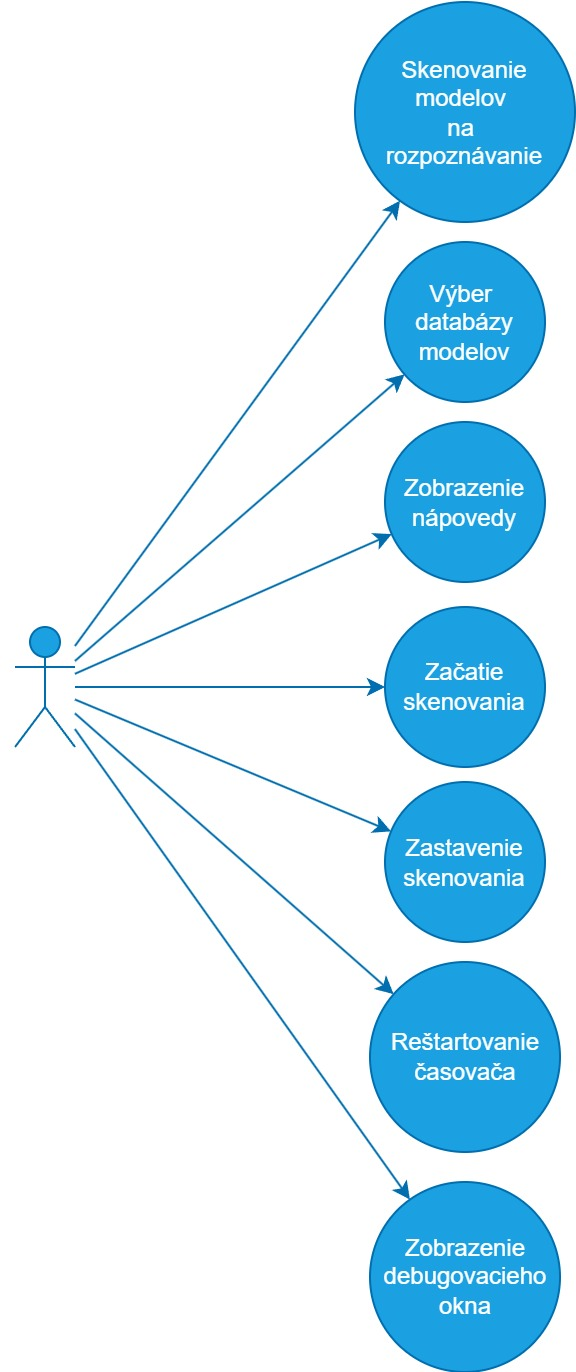
\includegraphics[width=0.4\textwidth]{img/use_case_diagram.jpg}
\caption{UML Use Case diagram aplikácie}
\label{fig:useCaseDiagram}
\end{figure}

V rámci implementácie aplikácie sme taktiež vytvorili manuál, vďaka ktorému si každý s prístupom na internet môže pridať vlastnú databázu s objektami, ktoré by chcel rozpoznávať. Manuál je priložený v~prílohe tejto diplomovej práce. V~aktuálnej verzii Vuforia knižnice nie je možné pridávať modely behom chodu aplikácie, Avšak, ak užívateľ má stiahnuté Unity, Model Target Generator, modely v~3D súborovom formáte a vytlačené modely, ktoré sú aspoň približne rovnakej veľkosti v~porovnaní s ich digitálnou kópiou, môže užívateľ veľmi jednoducho natrénovať vlastnú databázu s modelmi a následne ju naimportovať do Unity. Potom mu už stačí len vytvoriť nový build aplikácie a môže začať s identifikáciou jednotlivých modelov. 

Kódové príklady prezentované v~tejto diplomovej práci predstavujú základnú štruktúru originálneho kódu. Z dôvodu úspory miesta a zamerania na kľúčové aspekty implementácie boli vynechané niektoré podrobnosti, ako napríklad kontrola nulových ukazovateľov a iné bezpečnostné podmienky, ktoré sú súčasťou kompletného kódu. V~tejto práci sú poskytnuté len vybrané segmenty kódu, aby bolo možné demonštrovať jeho základnú funkcionalitu a štruktúru. 

\begin{figure}[h]
  \centering
  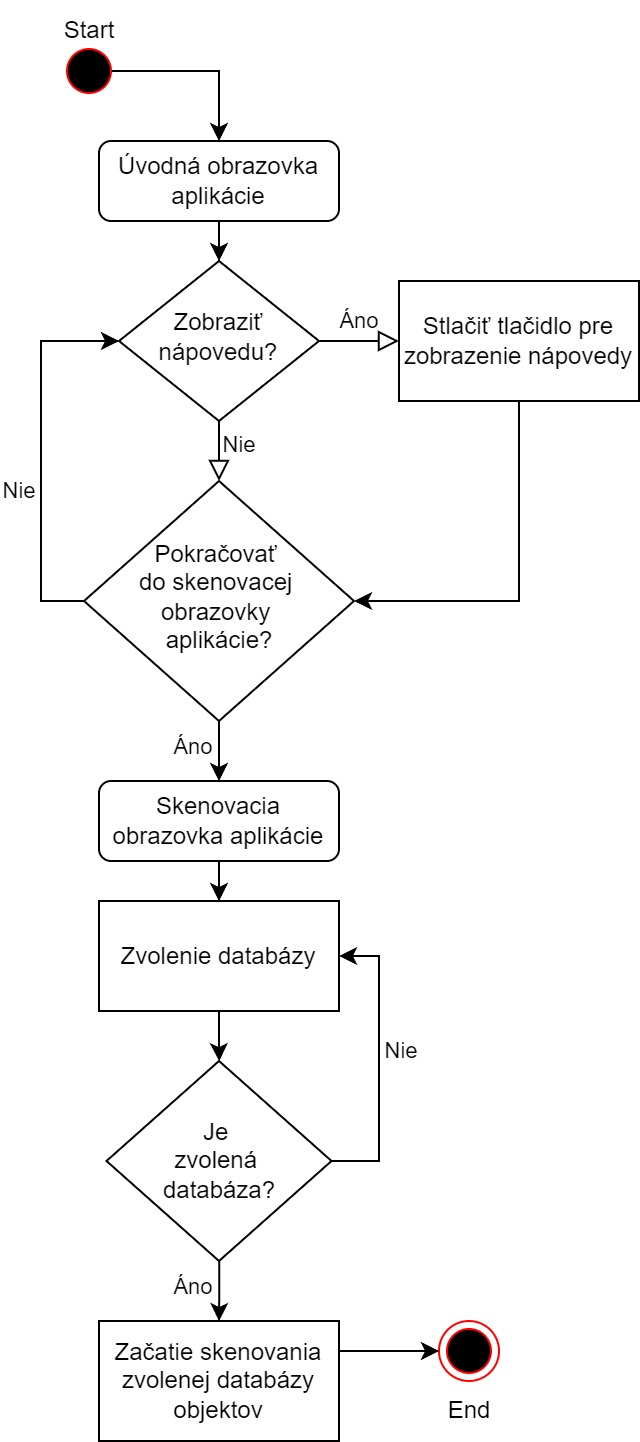
\includegraphics[width=0.6\textwidth]{img/diagram_aktivit.jpg}
  \caption{Diagram aktivity aplikácie}
  \label{fig:flowChart}
\end{figure}

\FloatBarrier 

\subsubsection{Úvodná obrazovka aplikácie} 

V tejto sekcii si popíšeme do detailov, k čomu nám úvodná obrazovka aplikácie slúži, popíšeme si jednotlivé UI elementy a skripty, ktoré táto obrazovka zahŕňa.

%DOPLNENE

\subsubsubsection{Opis úvodnej obrazovky aplikácie}

Na obrázku \ref{fig:introductionScene} môžeme vidieť všetky prvky úvodnej aplikácie. V~ďalšom odseku budeme teda vždy odkazovať na tento obrázok, avšak budeme spomínať očíslované jednotlivé prvky. Tieto prvky sú označené na obrázku červeným kruhom, v~ktorom sa nachádza číslo daného prvku. 

Pri spustení aplikácie sa nám zobrazí úvodná scéna aplikácie s uvítacím textom, viď obrázok \ref{fig:introductionScene}, číslo 1., tlačidlom na spustenie aplikácie a začatie skenovania, viď obrázok \ref{fig:introductionScene}, číslo 2, toto tlačidlo má v~sebe text „START SCANNING“ a nachádza sa v~strede obrazovky. Nachádza sa tu taktiež tlačidlo na zobrazenie vyskakovacieho okna s krátkou nápovedou, viď obrázok \ref{fig:introductionScene}, číslo 4, ako aplikáciu používať a aké podmienky je potrebné mať pre najlepšie rozpoznávanie vytlačených 3D objektov. Vyskakovacie okno, viď obrázok \ref{fig:introductionScene}, číslo 3 je nastavené tak, aby samo zmizlo po 10 sekundách alebo keď užívateľ znovu stlačí tlačidlo. Toto tlačidlo je označené písmenom „i“ a jedná sa o malé okrúhle tlačidlo v~pravom dolnom rohu.

\begin{figure}[h]
  \centering
  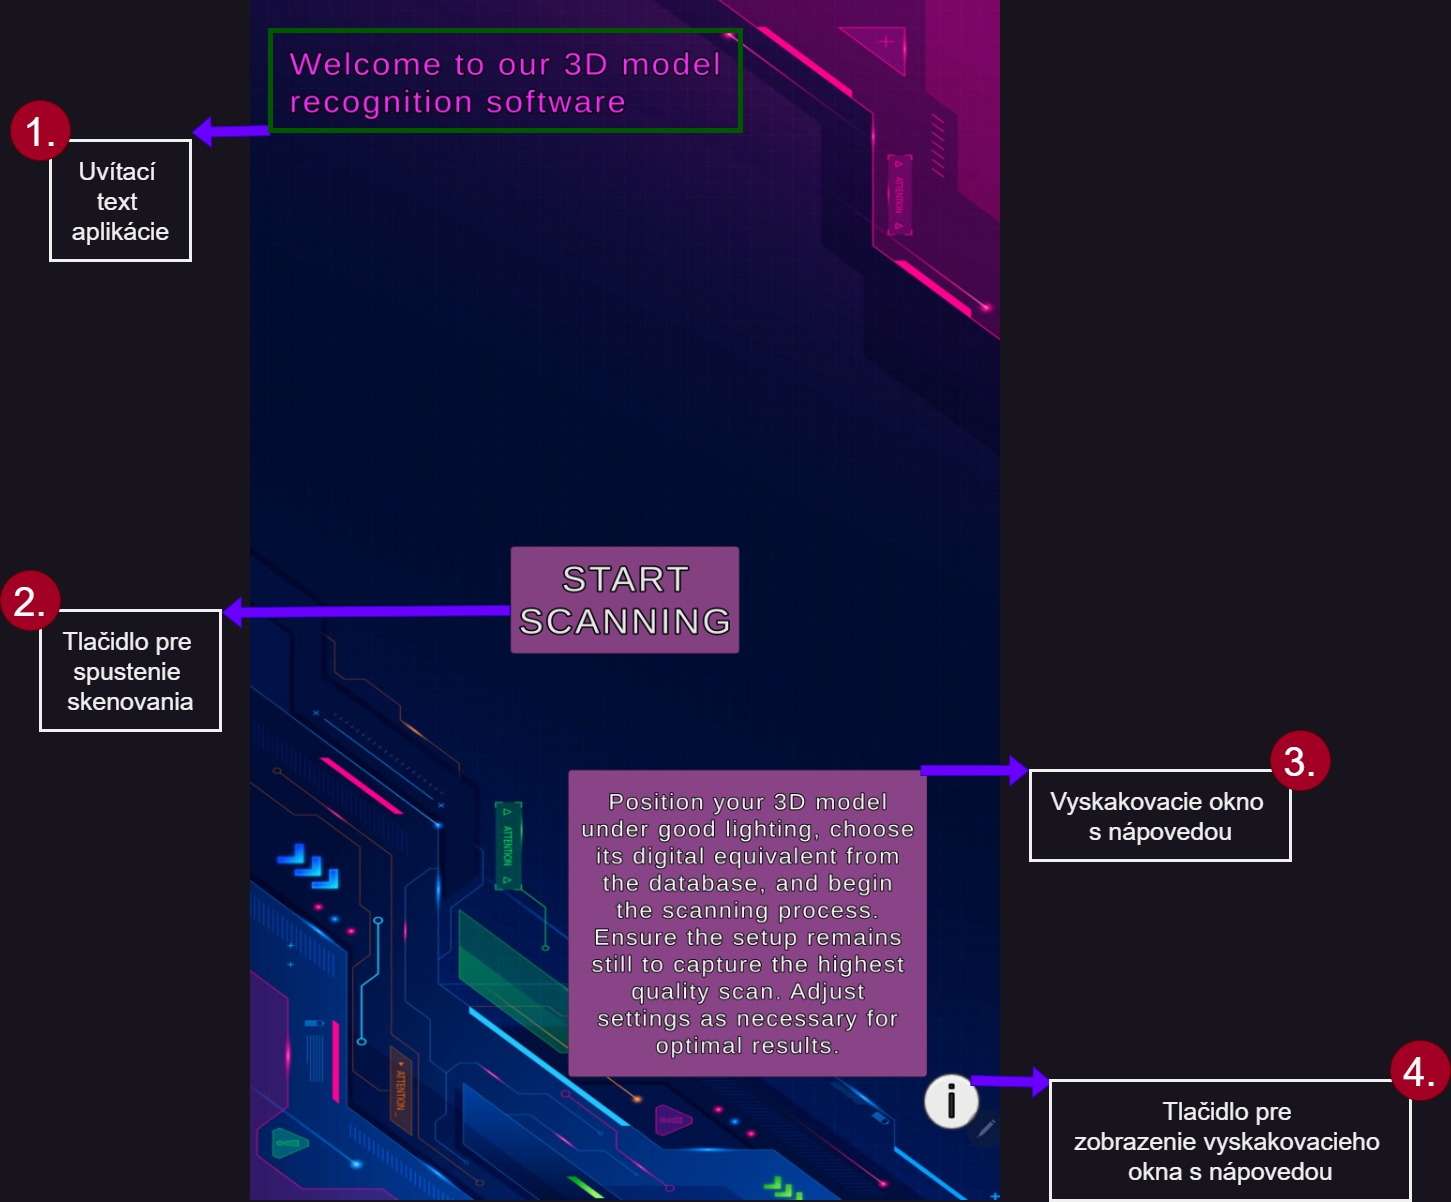
\includegraphics[width=0.9\textwidth]{img/Introduction_scene.jpg}
  \caption{Úvodná obrazovka aplikácie}
  \label{fig:introductionScene}
\end{figure}

\subsubsubsection{Vysvetlenie skriptov úvodnej obrazovky aplikácie}

Táto obrazovka využíva 2 skripty. Všetky skripty máme v~tejto scéne zastrešené pod objektom GameController, ten potom napájame k Unity eventu priamo v~Editore na OnClick(). Tlačidlo HelpButton používa skript TooltipManager a funkciu OnHelpButtonClick. Táto funkcia bude popísaná nižšie. Druhé tlačidlo StartButton, ktoré slúži na začatie skenovania Používa skript SceneLoader a funkciu LoadSceneByIndex. 

Na obrázku \ref{fig:introductionSceneStructure} je naša štruktúra Unity scény. Nachádza sa tam základná kamera so svetlom, plátno, na ktorom sa nachádzajú všetky UI prvky, teda tlačidlá, vyskakovacie okno, text a pozadie aplikácie + Event systém, ktorý Canvas používa. Taktiež sa tu nachádza spomínaný GameController, v~ktorom sú všetky potrebné skripty.  

\begin{figure}[h]
  \centering
  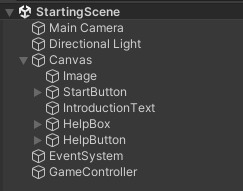
\includegraphics[width=0.3\textwidth]{img/structure_introduction.png}
  \caption{Štruktúra úvodnej scény aplikácie}
  \label{fig:introductionSceneStructure}
\end{figure}

{\normalsize\textbf{SceneLoader Class - Načítavanie scén}}

Prvý, veľmi jednoduchý skript nám prepína medzi scénami. Tento skript využívame taktiež aj v~druhej obrazovke, spôsob využitia v~druhej scéne si popíšeme v~ďalšej kapitole. Jedná sa o to, že každá obrazovka v~Unity je obalená v~scéne. Obsahuje všetky UI elementy, konfigurácie skriptov, nastavenie obrazovky a rôzne parametre. V~Unity máme pripnutý skript v~objekte GameController, ten následne používa tlačidlo spomenuté vyššie - Start scanning s parametrom sceneIndex 1. Použitím classy SceneManager.LoadScene(sceneIndex) takto môžeme prepínať medzi scénami. %EK: Klasy??? - opravene

Tento skript zároveň používame aj v~Skenovacej obrazovke aplikácie na návrat zo skenovacej scéne späť na úvodnú scénu aplikácie.

\lstset{style=Csharp}
\begin{lstlisting}[caption={SceneLoader Class - Načítavanie scén}, label=sceneLoader]
public void LoadSceneByIndex(int sceneIndex)
{
    SceneManager.LoadScene(sceneIndex);
}
\end{lstlisting}

{\normalsize\textbf{TooltipManager Class - Zobrazovanie vyskakovacieho pomocného poľa.}}

Druhý skript obsahuje funkcie Awake, Start, ToggleTooltip, ShowTooltipForDuration, PositionTooltip, StopAndHideTooltip a OnHelpButtonClick. V~prvej časti kódu si vysvetlíme bližšie prvé tri funkcie a parametre, ktoré používame v~tomto skripte. 

Prvá časť je deklarácia parametrov, \_instance, ktorú používame vo funkcii Awake. Táto funkcia slúži na to, aby sme mali len jeden TooltipManager v~našej scéne. 

Následne máme tooltipPanel, to je \gls{ui} panel pre samotné vyskakovacie okno, s ktorým následne potrebujeme pracovať tak, aby sme ho mohli cez skript zobraziť alebo skryť a aby bol odsadený v~dostatočnej vzdialenosti od buttonu. To budeme bližšie popisovať vo funkcii PositionTooltip. Aby sme toto okno nemali zobrazené na začiatku nastavujeme tento panel pomocou funkcie SetActive na False.

Vo funkcii ToggleTooltip využívame parametre displayCoroutine a lastButtonTransform. Premenná displayCoroutine nám uchováva Coroutine, keďže Unity nevie priamo pracovať s Threadmi, takto nám umožňuje začať odpočet desiatich sekúnd pre skrytie vyskakovacieho okna. Objekt buttonTransform nám slúži na uchovanie samotného tlačidla pre spustenie vyskakovacieho okna. Taktiež touto funkciou umožňujeme stlačením tlačidla znovu zastaviť Coroutinu. Ako to funguje popíšeme do hĺbky nižšie.

\lstset{style=Csharp}
\begin{lstlisting}[caption={TooltipManager Class - Zobrazovanie vyskakovacieho pomocného poľa. Part 1}, label=tooltipManagerPart1]
private void Awake()
{
    if (_instance != null && _instance != this)
    {
        Destroy(this.gameObject);
    }
    else
    {
        _instance = this;
    }
}

void Start()
{
    tooltipPanel.SetActive(false);
}

public void ToggleTooltip(Transform buttonTransform)
{
    lastButtonTransform = buttonTransform; 
    if (tooltipPanel.activeSelf)
    {
        StopAndHideTooltip(); 
    }
    else
    {
        if (displayCoroutine != null)
        {
            StopCoroutine(displayCoroutine); 
        }
        displayCoroutine = StartCoroutine(ShowTooltipForDuration(10));
    }
}
\end{lstlisting}

V druhej časti skriptu máme samotnú Coroutinu ShowtooltipForDuration s parametrom duration, ktorá nám odkazuje na to, ako dlho má byť zobrazené vyskakovacie okno. Zároveň tam zapíname spomínané vyskakovacie okno a po danom časovom úseku voláme funkciu StopAndHideTooltip, kde toto okno skrývame a vypíname Coroutinu. Celá táto implementácia je založená na tom, že užívateľ nemusí čakať určitý časový úsek, ale môže stlačením tlačidla znovu prerušiť časovač a skryť toto okno. Na zrušenie časovača sa používa natívna Unity funkcia StopCoroutine.

V poslednej funkcií je samotná funkcia tohoto tlačidla, tá volá len funkciu ToggleTooltip, ktorú sme si už popísali vyššie.

\lstset{style=Csharp}
\begin{lstlisting}[caption={TooltipManager Class - Zobrazovanie vyskakovacieho pomocného poľa. Part 2}, label=tooltipManagerPart2]
private IEnumerator ShowTooltipForDuration(float duration)
{
    PositionTooltip();
    tooltipPanel.SetActive(true); 
    yield return new WaitForSeconds(duration); 
    StopAndHideTooltip(); 
}

private void PositionTooltip()
{
    tooltipPanel.transform.position = lastButtonTransform.position + offset;
}

private void StopAndHideTooltip()
{
    if (displayCoroutine != null)
    {
        StopCoroutine(displayCoroutine);
        displayCoroutine = null;
    }
    tooltipPanel.SetActive(false);
}

public void OnHelpButtonClick(Button button)
{
    TooltipManager._instance.ToggleTooltip(button.transform);
}
\end{lstlisting}

\subsubsection{Skenovacia obrazovka aplikácie}

V tejto sekcii si popíšeme Skenovaciu obrazovku aplikácie. Do detailov vysvetlíme všetky skripty v~tejto scéne, všetky tlačidlá, textové elementy a okná a vysvetlíme, ako aplikácie celkovo funguje. %EK: Scripty vsade prepisat na slovenske skripty. Nie je to dovod to pisat takto. - OPRAVENE

%DOPLNENE

\subsubsubsection{Popis skenovacej obrazovky aplikácie}

V tejto scéne sa nachádzajú všetky hlavné funkcionality aplikácie. Užívateľ si najprv musí zvoliť databázu, ktorá je vopred implementovaná v~builde aplikácie, tento rozbaľovací list sa nachádza na obrázku \ref{fig:scanningScene2}, pod číslom 1. Následne je potrebné stlačiť tlačidlo pre spustenie skenovania, toto tlačidlo môžeme vidieť na obrázku \ref{fig:scanningScene2} pod číslom 2. Týmto tlačidlom sa načítajú modely z databázy a aplikácia začne skenovanie. Skenovanie a identifikácia začne hneď po tom, čo sa modely dynamicky načítajú do scény a kamerou sa aplikácia snaží hľadať tieto modely až kým užívateľ nepreruší chod aplikácie zmenením databázy, zastavením skenovania, vrátenia sa do úvodnej obrazovky ale vymazaním modelov v~scéne. 

Rozbaľovací list a tlačidlo pre vybratie databázy nám zmizne z obrazovky, aby zbytočne nezaberalo miesto behom skenovania objektov kamerou. 

\begin{figure}[!h]
  \centering
  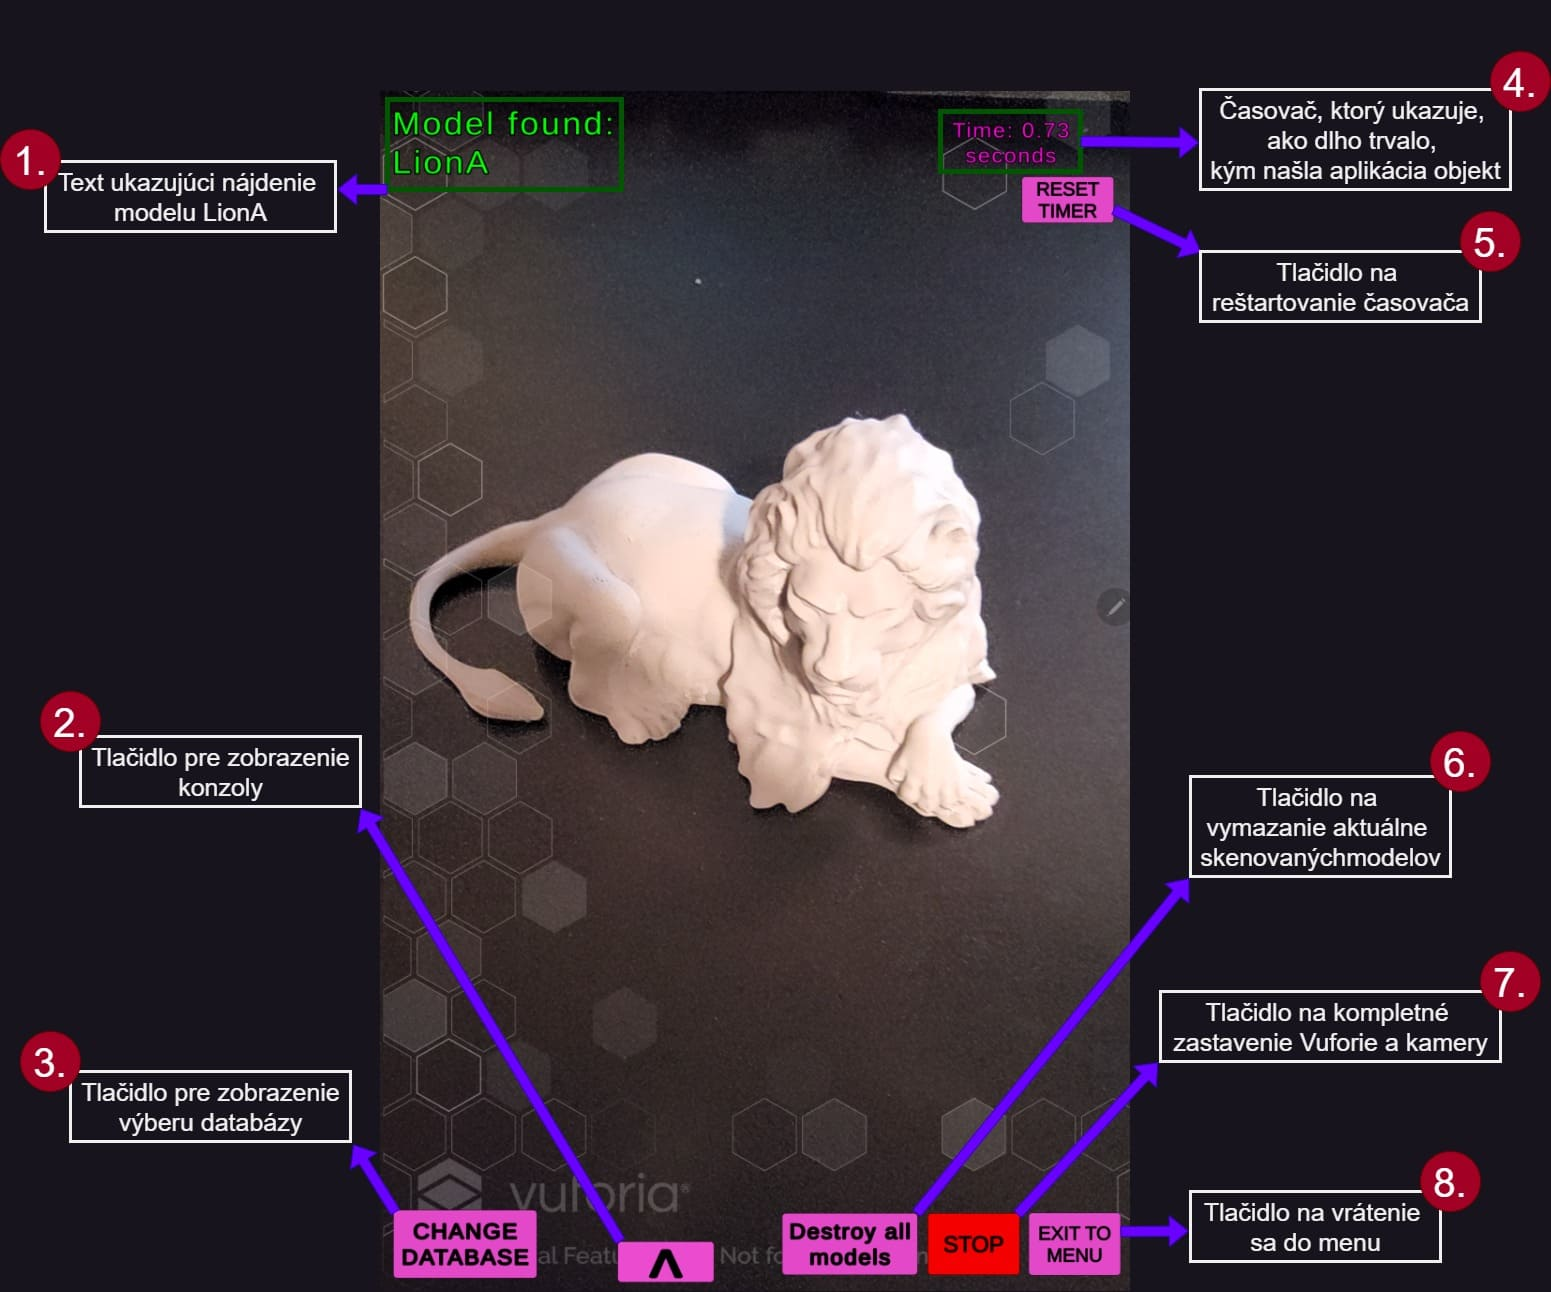
\includegraphics[width=1\textwidth]{img/Scanning_scene_part1.jpg}
  \caption{Štruktúra skenovacej scény aplikácie}
  \label{fig:scanningScene1}
\end{figure}

Zastaviť skenovanie môžeme celkom tromi spôsobmi. Prvým spôsobom je stlačením tlačidla Destroy all models, toto tlačidlo môžeme vidieť na obrázku \ref{fig:scanningScene1}, pod číslom 6. Stlačením tohoto tlačidla, ako názov naznačuje, vymažeme dynamicky vytvorené modely, ktoré sa vytvorili po tom, čo sme si vybrali databázu. Týmto zastavíme skenovanie aplikácie, pričom nám zostáva zapnutá kamera a aplikácia čaká, kým si zvolíme databázu, aby mohla znovu začať skenovanie.

Druhým spôsobom, ako zastaviť skenovanie môžeme stlačením tlačidla STOP, toto tlačidlo sa nachádza na obrázku \ref{fig:scanningScene1}, pod číslom 7. Stlačením tohoto tlačidla zastavíme kompletne beh Vuforia enginu v~našej aplikácií. To však znamená, že prerušíme aj chod AR kamery, ktorú Vuforia používa. Znovu môžeme Vuforia engine inicializovať stlačením tlačidla START, toto tlačidlo môžeme vidieť na obrázku \ref{fig:scanningScene2}, pod číslom 5. Tlačidlo je nastavené tak, že ak aplikácia beží je možné stlačiť tlačidlo STOP s červeným pozadím, ak aplikácia je zastavená tlačidlo sa zmení na START so zeleným pozadím.

Tretím spôsobom, ako zastaviť skenovanie je stlačením tlačidla EXIT TO MENU. Toto tlačidlo môžeme vidieť na obrázku \ref{fig:scanningScene1}, pod číslom 8. Týmto tlačidlom sa vrátime na úvodnú obrazovku aplikácie, ktorá bola spomínaná vyššie. 

\begin{figure}[!h]
  \centering
  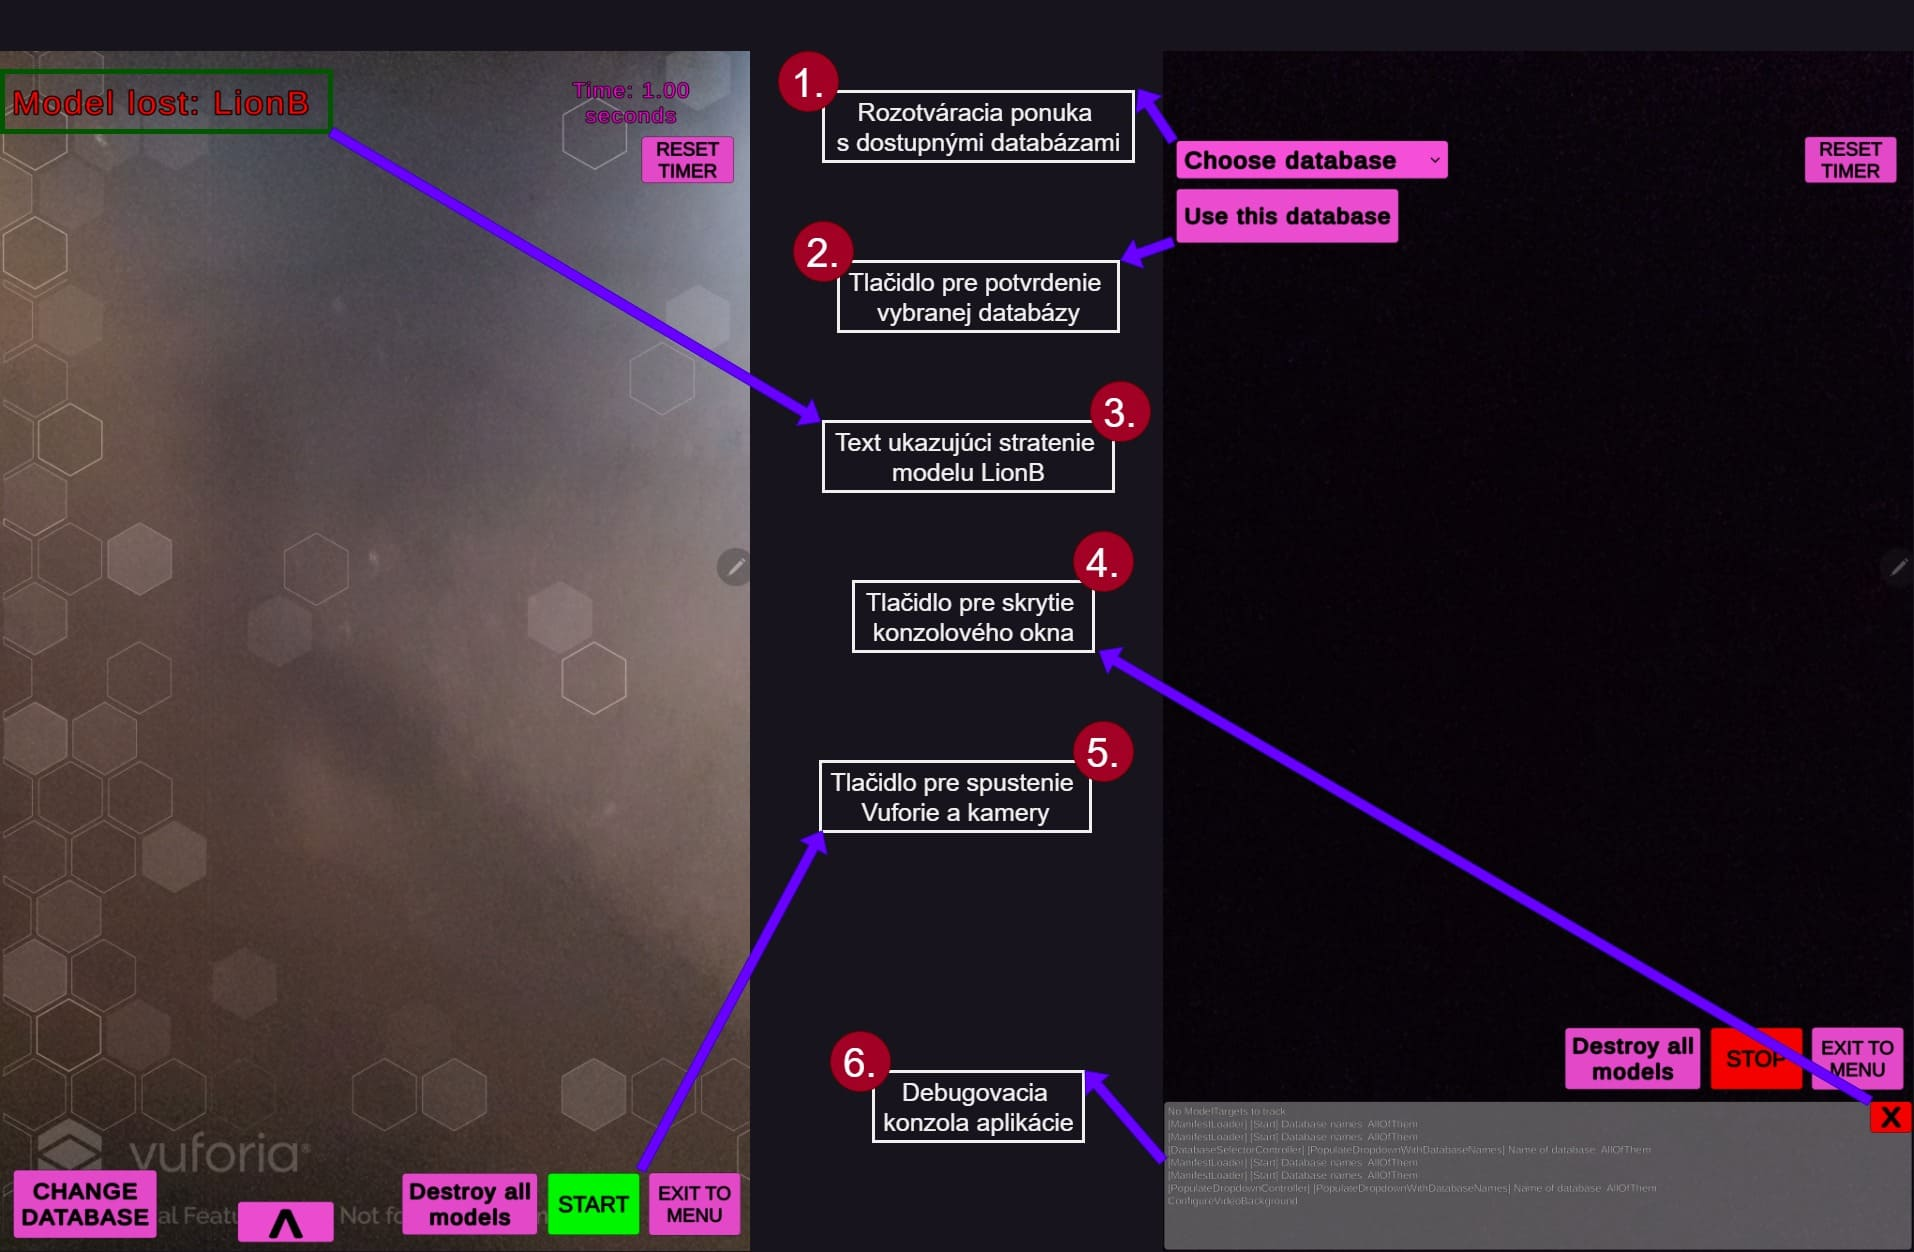
\includegraphics[width=1\textwidth]{img/Scanning_scene_part2Collapse.jpg}
  \caption{Štruktúra skenovacej scény aplikácie}
  \label{fig:scanningScene2}
\end{figure}

Počas skenovania sa na obrazovke nachádza časovač, ktorý môžeme vidieť na obrázku \ref{fig:scanningScene1}, pod číslom 4, ktorý počíta koľko sekúnd ubehlo od začatie skenovania, ten sa zastaví akonáhle nájde model a znovu sa spustí keď aplikácia model „stratí“, napríklad tým, že modelom začneme rýchlo hýbať alebo ho dáme mimo záberu kamery. Taktiež je možné časovač reštartovať tlačidlom Reset Timer, ak to situácia vyžaduje, toto tlačidlo môžeme vidieť na obrázku \ref{fig:scanningScene1}, pod číslom 5. 

Ak chceme zmeniť databázu objektov počas už začatého skenovania s inou databázou, je tak možné urobiť stlačením tlačidla CHANGE DATABASE, toto tlačidlo môžeme vidieť na obrázku \ref{fig:scanningScene1}, pod číslom 3. Stlačením tohoto tlačidla sa nám znovu zobrazí rozbaľovací list s importovanými databázami objektov a taktiež sa zobrazí tlačidlo pre vybratie databázy. Následne stačí užívateľovi zvoliť si databázu a stlačiť tlačidlo pre použitie zvolenej databázy. Aby používateľ mohol zmeniť databázu, nie je potrebné predtým zmazať aktuálne používane modely, ani akýkoľvek iný úkon. Stačí len vybrať databázu, potvrdiť tlačidlom a aplikácia sama vymaže aktuálne modely a nahradí ich novo vybratou databázou.

V aplikácii sa taktiež, kvôli testovacím potrebám, nachádza konzola. Keďže mnohé veci fungujú trochu inak v~Unity editore a inak priamo na zariadení, bolo nutné pre nájdenie a vyladenie chýb vytvoriť debugovaciu konzolu. V~tejto konzole si developer môže vypisovať rôzne hlášky a premenne, ktoré by chcel vidieť priamo na zariadení. Popis, ako to môže urobiť budeme podrobne vysvetľovať v~nasledujúcej sekcii. Aby užívateľovi táto konzola nezavadziala, ak ju nepotrebuje práve používať, je zo základu skrytá. Zobraziť ju môžeme stlačením tlačidla, ktoré sa nachádza na obrázku \ref{fig:scanningScene1}, pod číslom 2. Stlačením sa nám teda zobrazí spomínaná konzola a tlačidla, ktoré sa nachádzajú na spodku aplikácie, sa posunú automaticky nad ňu. Konzolu môžeme znovu skryť stlačením tlačidla X, ktoré môžeme vidieť na obrázku \ref{fig:scanningScene2}, pod číslom 4. Týmto tlačidlom sa konzola skryje a tlačidla sa vrátia na pôvodné miesto.

\FloatBarrier 

\subsubsubsection{Popis skriptov skenovacej obrazovky aplikácie}

Na obrázku \ref{fig:scanningSceneStructure} môžeme vidieť štruktúru skenovacej obrazovky aplikácie. Nachádza sa tu AR kamera, ktorá je súčasťou knižnice Vuforia. Prostredníctvom tejto kamery dokážeme skenovať objekty, keďže kamera je prepojená priamo s Vuforiou odosiela informácie z kamery do knižnice a tá následne vyhodnocuje výsledky pri skenovaní. V~objekte Canvas sa nachádzajú všetky UI elementy aplikácie, tie si popíšeme v~odsekoch nižšie. Taktiež sa tu nachádza prázdny objekt ModelContainer, ktorý slúži len, ako kontajner pre dynamicky vytvorené objekty s Vuforia komponentami, ktoré sa vytvoria po zvolení databázy na skenovanie. Tieto objekty sa následne porovnávajú s vstupom AR kamery.   

\begin{figure}[h]
  \centering
  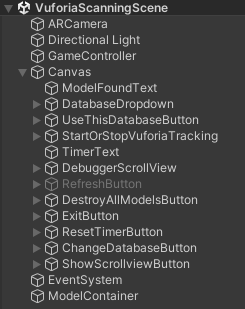
\includegraphics[width=0.3\textwidth]{img/structure_scanning.png}
  \caption{Štruktúra skenovacej scény aplikácie}
  \label{fig:scanningSceneStructure}
\end{figure}

V poslednej verzii aplikácie sa tu nachádza dokopy 12 objektov, všetky budú spomenuté do hĺbky nižšie. Z dvanástich objektov máme 1 skrolovacie textové pole DebuggerScrollView, 2 textové polia ModelFoundText a TimerText, 1 dropdown DatabaseDropdown a 8 tlačidiel, z ktorých každý plní nejakú úlohu v~aplikácií, sú to UseThisDatabaseButton, StartOrStopVuforiaTrackingButton, RefreshButton, DestoryAllModelsButton, ExitButton, ResetTimerButton, ChangeDatabaseButton a ShowScrollviewButton. Jednotlivé UI objekty budú spomenuté a ich funkcie vysvetlené spolu s príslušnými skriptami, ktoré používajú. Všetky tieto objekty môžeme vidieť na obrázku \ref{fig:scanningSceneStructure} pod objektom Canvas. V~tomto plátne sa nachádzajú všetky UI prvky aplikácie.

Scéna skenovacej obrazovky aplikácie, rovnako, ako úvodná scéna aplikácie, sú skripty zastrešené pod objektom GameController, tento môžeme vidieť na obrázku \ref{fig:scanningSceneStructure}, na ktorý sa následne napájajú jednotlivé tlačidlá alebo fungujú pasívne behom skenovania aplikácie. V~tejto doméne využívame pätnásť skriptov, z toho jeden sme už spomenuli v~kapitole vyššie, to je SceneLoader. Skript SceneLoader, ktorého kód je v~algoritme \ref{sceneLoader}, je spojený s tlačidlom EXIT TO MENU. Slúži na pozastavenie skenovania aplikácie, prípadne ak nechceme už mať naďalej zapnutú kameru alebo si chceme pozrieť nápovedu na Úvodnej obrazovke aplikácie. Stlačením tlačidla sa teda vraciame na Úvodnú obrazovku aplikácie. 

{\large\textbf{Skript ChangeDatabaseController}}

Ďalším skriptom je ChangeDatabaseController, algoritmus je pod číslom \ref{changeDatabaseController}. Tento skript zastrešuje funkciu systému, ktorý umožňuje používateľom výber a zmenu databázy v~grafickom používateľskom rozhraní (GUI). Skript je priradený k GameObjectu a ovláda interakciu s komponentami GUI, ako sú tlačidlá a rozbaľovacie menu, na základe výberu používateľa. Vysvetlime si hlavné časti kódu:

{\small\textbf{Inicializácia a nastavenie GUI komponentov}}

Pri štarte aplikácie sa v~metóde Start() najprv nastaví viditeľnosť grafických komponentov:

\begin{itemize}
    \item DatabaseDropdown a UseThisDatabaseButton sú nastavené na viditeľné, čo umožňuje používateľovi ihneď vybrať databázu.
    \item ChangeDatabaseButton je nastavený na neviditeľný, pretože na začiatku nie je potrebné databázu meniť.
\end{itemize}

{\small\textbf{Správa komponentov Dropdown}}

Skript tiež získava komponent TMP\_Dropdown priradený k objektu DatabaseDropdown. Tento komponent obsahuje rozbaľovacie menu, ktoré umožňuje používateľom vyberať z rôznych dostupných databáz.

{\small\textbf{Priradenie funkcií tlačidlám}}

Tlačidlá UseThisDatabaseButton a ChangeDatabaseButton majú priradené poslucháče kliknutí, ktoré vyvolajú metódy OnUseThisDatabaseClicked() a OnChangeDatabaseClicked(). Tieto metódy definujú, čo sa stane po kliknutí na tlačidlá.

{\small\textbf{Funkcia OnUseThisDatabaseClicked}}

Táto metóda reaguje na výber databázy z rozbaľovacieho menu. Ak používateľ vyberie inú, ako predvolenú možnosť (kde predvolená možnosť má index 0), skript skryje DatabaseDropdown a UseThisDatabaseButton, a zobrazí ChangeDatabaseButton. To umožňuje používateľovi neskôr zmeniť svoj výber. Ak je vybraná predvolená možnosť, skript zaloguje správu, aby používateľ vybral inú databázu.

{\small\textbf{Funkcia OnChangeDatabaseClicked}}

Táto metóda je vyvolaná, keď používateľ klikne na ChangeDatabaseButton, čo spôsobí skrytie tohto tlačidla a znovu-zobrazenie DatabaseDropdown a UseThisDatabaseButton pre nový výber.

\lstset{style=Csharp}
\begin{lstlisting}[caption={ChangeDatabaseController Class - Zmena skenovacej databázy aplikácie}, label=changeDatabaseController]
void Start()
{
    DatabaseDropdown.SetActive(true);
    UseThisDatabaseButton.SetActive(true);
    ChangeDatabaseButton.SetActive(false);
    databaseDropdownComponent = DatabaseDropdown.GetComponent<TMP_Dropdown>();
    UseThisDatabaseButton.GetComponent<Button>().onClick.AddListener(() => OnUseThisDatabaseClicked());
    ChangeDatabaseButton.GetComponent<Button>().onClick.AddListener(() => OnChangeDatabaseClicked());
}

void OnUseThisDatabaseClicked()
{
    UseThisDatabaseButton.SetActive(false);
    DatabaseDropdown.SetActive(false);
    ChangeDatabaseButton.SetActive(true);
}

void OnChangeDatabaseClicked()
{
    ChangeDatabaseButton.SetActive(false);
    DatabaseDropdown.SetActive(true);
    UseThisDatabaseButton.SetActive(true);
}
\end{lstlisting}

{\large\textbf{Skript CustomObserverEventHandler}}

Tento kód v~jazyku C\# definuje triedu CustomObserverEventHandler, ktorá rozširuje funkčnosť štandardnej triedy DefaultObserverEventHandler z Vuforia SDK v~prostredí Unity. Táto trieda je navrhnutá na zvládnutie udalostí, keď je objekt v~rozšírenej realite nájdený alebo stratil sledovanie.

\begin{itemize}
    \item {\small\textbf{Udalosti}}: Trieda má dve verejné akcie, OnModelFound a OnModelLost, ktoré umožňujú priradenie vlastných funkcií na spracovanie týchto udalostí. Tieto akcie sú volané s menom GameObjectu, ktorý bol nájdený alebo stratený.
    \item {\small\textbf{Metóda OnTrackingFound}}: Prepísaná metóda, ktorá po úspešnom získaní sledovania objektu, vyvolá akciu OnModelFound.
    \item {\small\textbf{Metóda OnTrackingLost}}: Pri strate sledovania vyvoláva akciu OnModelLost.
\end{itemize}

Táto funkcionalita je dôležitá pre aplikácie rozšírenej reality, pretože umožňuje dynamickú reakciu na zmeny v~sledovaní objektov, čo zvyšuje interaktivitu a používateľský zážitok. Kód demonštruje, ako môžu byť prispôsobené reakcie aplikácie na udalosti sledovania využitím Vuforia SDK.

\lstset{style=Csharp}
\begin{lstlisting}[caption={CustomObserverEventHandler Class - rozšírenie knižnice Vuforia}, label=]
public class CustomObserverEventHandler : DefaultObserverEventHandler
{
    public System.Action<string> OnModelFound;
    public System.Action<string> OnModelLost;

    protected override void OnTrackingFound()
    {
        base.OnTrackingFound();
        OnModelFound?.Invoke(gameObject.name);
    }

    protected override void OnTrackingLost()
    {
        base.OnTrackingLost();
        OnModelLost?.Invoke(gameObject.name);
    }
}
\end{lstlisting}

{\large\textbf{Skript ModelFoundController}}

Skript ModelFoundController je určený na ovládanie správ, ktoré sa zobrazujú na užívateľskom rozhraní, keď sú modely v~AR aplikácii nájdené alebo stratené. Skript využíva viacero komponentov Unity a Vuforia.

Skript využíva sériovo pripojené polia pre komponenty TMP\_Text a StartStopButtonController. TMP\_Text je komponenta z TextMesh Pro, ktorá umožňuje zobraziť upravený text v~Unity. StartStopButtonController je vlastná komponenta, ktorá ovláda štartovacie a zastavovacie tlačidlá aplikácie, reaguje na stavy nájdenia alebo stratenia modelu.

Hlavné metódy NewModelFound a ModelLost sú volané, keď aplikácia zistí prítomnosť alebo neprítomnosť AR modelu. Metóda NewModelFound sa aktivuje, keď je model nájdený. Táto metóda informuje komponent StartStopButtonController o náleze modelu a spustí korutinu, ktorá zobrazuje správu o nájdení modelu v~zelenom farebnom kóde. Podobne, metóda ModelLost reaguje na stratu modelu zobrazením červenej správy a informuje StartStopButtonController o strate modelu.

Korutina DisplayMessageTemporarily je zodpovedná za dočasné zobrazenie správ. Táto metóda nastaví text a farbu TMP\_Text komponenty, čaká požadovaný čas (v tomto prípade 3 sekundy) a potom vymaže text. Tento prístup je užitočný na to, aby používateľovi poskytol okamžitú spätnú väzbu, ale zároveň nezaplnil užívateľské rozhranie trvalými správami.

\lstset{style=Csharp}
\begin{lstlisting}[caption={ModelFoundController Class - Ovladanie správ pri nájdeni modelu}, label=changeDatabaseController]
public void NewModelFound(string gameObjectName)
{
    startStopButtonController.ModelFound();
    StartOrRestartMessageCoroutine($"Model found: {gameObjectName}", Color.green);
}

public void ModelLost(string gameObjectName)
{
    StartOrRestartMessageCoroutine($"Model lost: {gameObjectName}", Color.red);
    startStopButtonController.ModelLost();
}

private void StartOrRestartMessageCoroutine(string message, Color color)
{
    if (messageDisplayCoroutine != null)
    {
        StopCoroutine(messageDisplayCoroutine);
    }
    messageDisplayCoroutine = StartCoroutine(DisplayMessageTemporarily(message, color, 3f));
}

private IEnumerator DisplayMessageTemporarily(string message, Color color, float duration)
{
    modelFoundText.text = message;
    modelFoundText.color = color;
    yield return new WaitForSeconds(duration);
    modelFoundText.text = "";
    messageDisplayCoroutine = null;
}
\end{lstlisting} 

{\large\textbf{Skript ModelTargetDatabaseXmlReader}}

Tento kód je skript pre Unity, ktorý využíva UnityWebRequest a XML serializáciu na načítanie a spracovanie dát modelov cieľov zo súborov XML.Tu je podrobný rozbor hlavných častí a funkčnosti skriptu:

{\normalsize\textbf{Skript Stručný popis}}

Skript ModelTargetDatabaseXmlReader je komponentou Unity, ktorá poskytuje funkcie na načítanie databázy názvov cieľových modelov z viacerých XML súborov. Skript využíva asynchrónne načítanie pomocou korutín (coroutines) v~Unity, čo umožňuje efektívne načítanie bez blokovania hlavného vlákna aplikácie.

{\normalsize\textbf{Hlavné komponenty skriptu}}

\begin{itemize}
    \item {\small\textbf{XmlSerializer}}: Na deserializáciu XML súborov do objektov v~C\#. V~tomto prípade je typ deserializovaného objektu QCARConfig, ktorý obsahuje štruktúru konfigurácie databázy cieľových modelov. Je možné, že v~budúcnosti sa zmení štruktúra tohoto xml, preto bude potrebné v~budúucnosti ak sa naskytne takýto problém s parsovaním XML, poupraviť štruktúru aby znovu vyhohovala výstupu ModeLTargetGenerátora.
    \item {\small\textbf{GetAllModelTargetNames}}: Public metóda, ktorá inicializuje načítanie dát zadaných databáz pomocou korutíny. Funkcia prijíma zoznam názvov databáz a callback funkciu, ktorá sa vykoná po dokončení načítania.
    \item {\small\textbf{LoadModelTargets}}: Private korutína, ktorá asynchrónne načíta XML súbory a spracuje ich. Načítava súbory pomocou UnityWebRequest a po úspešnom načítaní sú dáta deserializované a pridané do slovníka, kde kľúčom je názov databázy a hodnotou je množina názvov ModelTargetov.
\end{itemize}

{\normalsize\textbf{Proces načítania a spracovania}}

Načítavanie začína zložením cesty k súboru XML založenej na preddefinovanom formáte a umiestnení v~adresárovej štruktúre projektu Unity. UnityWebRequest sa používa na asynchrónne načítanie súborov. Ak dôjde k chybe, generuje sa varovanie. V~opačnom prípade sa obsah súboru načíta a deserializuje. Každý úspešne načítaný objekt je potom prehľadaný na zistenie dostupných modelových cieľov, ktoré sa pridávajú do kolekcie.

{\normalsize\textbf{Ukončenie a Callback}}

Po dokončení načítania všetkých databáz sa výsledný slovník s dátami prenesie späť do volajúcej funkcie pomocou callbacku. Toto umožňuje flexibilné spracovanie dát po načítaní, napríklad aktualizáciu používateľského rozhrania alebo ďalšiu logiku aplikácie závislú od načítaných dát.

\lstset{style=Csharp}
\begin{lstlisting}[caption={ModelTargetDatabaseXmlReader Class - Čítanie databázy z xml súboru}, label=modelTargetDatabaseXmlReader]
XmlSerializer serializer = new XmlSerializer(typeof(QCARConfig));

public void GetAllModelTargetNames(List<string> databaseNames, System.Action<Dictionary<string, HashSet<string>>> onComplete)
{
    StartCoroutine(LoadModelTargets(databaseNames, onComplete));
}

private IEnumerator LoadModelTargets(List<string> databaseNames, System.Action<Dictionary<string, HashSet<string>>> onComplete)
{
    Dictionary<string, HashSet<string>> databaseModelTargets = new Dictionary<string, HashSet<string>>();
    foreach (var databaseName in databaseNames)
    {
        string path = Path.Combine(Application.streamingAssetsPath, $"Vuforia/{databaseName}.xml");
        UnityWebRequest www = UnityWebRequest.Get(path);
        yield return www.SendWebRequest();
        using (StringReader reader = new StringReader(www.downloadHandler.text))
        {
            QCARConfig qcarConfig = (QCARConfig)serializer.Deserialize(reader);
            if (!databaseModelTargets.ContainsKey(databaseName))
            {
                databaseModelTargets[databaseName] = new HashSet<string>();
            }
            if (qcarConfig.Tracking != null && qcarConfig.Tracking.ModelTargets != null)
            {
                foreach (var modelTarget in qcarConfig.Tracking.ModelTargets)
                {
                    databaseModelTargets[databaseName].Add(modelTarget.Name);
                }
            }
        }
        
    }
    onComplete?.Invoke(databaseModelTargets);
}
\end{lstlisting} 

{\large\textbf{Skript ManifestLoader}}

Tento skript slúži na načítanie názvov databáz z manifestového súboru pre modelové ciele Vuforia. Tento prístup je zásadný v~prípadoch, kedy sú databázy s modelovými cieľmi dynamicky pridávané do projektu Unity, a je potrebné ich manažovať efektívne bez nutnosti ručných zásahov do štruktúry aplikácie.

\begin{itemize}
    \item {\small\textbf{Inicializácia}}: Trieda ManifestLoader dedí z MonoBehaviour, čo je základný stavebný kameň každého Unity skriptu. Člen databaseNames je zoznam reťazcov, ktorý bude obsahovať názvy všetkých databáz uložených v~manifestovom súbore.
    \item {\small\textbf{Načítanie manifestu}}: Metóda GetAllDatabaseNamesFromManifest() začína načítaním textového súboru manifest pomocou metódy Resources.Load<TextAsset>(). Tento súbor obsahuje názvy databáz, ktoré boli do projektu importované. Použitie adresára Resources umožňuje Unity načítať súbory za behu, čo je kľúčové pre dynamickú správu obsahu.
    \item {\small\textbf{Spracovanie textu}}: Načítaný text z manifestu je rozdelený do zoznamu podľa nových riadkov a prázdných riadkov pomocou Split(), z ktorého sú odstránené všetky prázdne položky pomocou RemoveAll(). Táto čistota zabezpečuje, že žiadne prázdne alebo neplatné názvy sa nedostanú do finálneho zoznamu.
    \item {\small\textbf{Logovanie a správa chýb}}: Každý úspešne načítaný názov databázy je zalogovaný pomocou Debug.Log(), čo pomáha pri ladení a overovaní správneho načítania názvov. V~prípade neúspešného načítania manifestu vyvolá metóda Debug.LogError(), čo informuje vývojára o potenciálnej chybe pri hľadaní alebo načítaní súboru.
\end{itemize}

{\normalsize\textbf{Výhody a flexibilita prístupu}}

Tento prístup umožňuje jednoduché a rýchle pridávanie nových databáz do projektu Unity bez nutnosti manuálneho zapracovávania zmeny do kódu alebo aplikácie. Stačí importovať nový balíček databáz (unitypackage), zapísať názov databázy do manifestu a aplikácia je pripravená na rebuild s novým obsahom. Tento systém je veľmi flexibilný a užívateľsky prívetivý, čo je ideálne pre projekty, kde je očakávané časté aktualizovanie alebo rozširovanie databáz. To všetko bez potreby zložitých manipulácií so súbormi alebo štruktúrou projektu, čo je obzvlášť užitočné v~prostrediach, kde sú operačné systémy, ako je Android, obmedzené v~priamom prístupe k súborom v~adresári StreamingAssets.

\lstset{style=Csharp}
\begin{lstlisting}[caption={ManifestLoader Class - Čítanie databáz zo súboru Manifest}, label=manifestLoader]
public List<string> GetAllDatabaseNamesFromManifest()
{
    TextAsset manifestTextAsset = Resources.Load<TextAsset>("manifest");
    databaseNames = new List<string>(manifestTextAsset.text.Split(new[] { '\r', '\n' }, StringSplitOptions.RemoveEmptyEntries));
    databaseNames.RemoveAll(string.IsNullOrEmpty);

    foreach (string databaseName in databaseNames)
    {
        Debug.Log("[ManifestLoader] [Start] Database names: " + databaseName);
    }
    return databaseNames;
}
\end{lstlisting} 

{\large\textbf{Vlastná konzola pre debugovanie v~aplikácií}}

V tejto časti sa budem venovať implementácii vlastnej konzoly, ktorá slúži na efektívne logovanie chýb a správ v~prostredí mobilných zariadení. Táto funkcionalita sa ukázala ako kritická, keďže tradičné metódy debuggovania aplikácií v~prostredí desktopových počítačov často nepostačujú pri riešení problémov, ktoré sa vyskytujú len na mobilných zariadeniach po vykonaní buildu. Zvlášť v~prípadoch, keď aplikácia na desktopovej verzií funguje bez problémov, avšak na mobilnom zariadení sa vyskytujú neočakávané chyby alebo správanie.

{\normalsize\textbf{ExceptionLogger}}

Prvým krokom v~implementácii je vytvorenie triedy ExceptionLogger, ktorá obsahuje statickú metódu BuildExceptionMessage. Táto metóda je zodpovedná za rekurzívne zostavenie detailného logu výnimky vrátane jej vnútorných výnimiek. Tento log je potom možné jednoducho zobraziť alebo uložiť pre neskoršiu analýzu. V~praxi využíva StringBuilder na zostavenie textového reťazca obsahujúceho relevantné informácie o každej úrovni výnimky, čo umožňuje hlbšiu analýzu problémov.

\lstset{style=Csharp}
\begin{lstlisting}[caption={ExceptionLogger Class - Vytvorenie custom debug správy}, label=exceptionLogger]
public static string BuildExceptionMessage(Exception exception)
{
    StringBuilder sb = new StringBuilder();
    sb.AppendLine("Exception caught:");
    Exception currentException = exception;
    int exceptionLayer = 0; 
    while (currentException != null)
    {
        sb.AppendLine($"Exception Layer {exceptionLayer}: {currentException.GetType().FullName}");
        sb.AppendLine($"Message: {currentException.Message}");
        sb.AppendLine($"StackTrace: {currentException.StackTrace}");
        currentException = currentException.InnerException;
        exceptionLayer++;
        if (currentException != null)
        {
            sb.AppendLine($"--- Inner Exception {exceptionLayer} ---");
        }
    }
    return sb.ToString();
}

public static void LogException(Exception ex)
{
    string detailedErrorMessage = BuildExceptionMessage(ex);
    Debug.LogError(detailedErrorMessage);
}
\end{lstlisting} 

{\normalsize\textbf{DebugUI}}

Druhým dôležitým komponentom je DebugUI, ktorý sa stará o vizuálne zobrazenie logov v~užívateľskom rozhraní mobilného zariadenia. Táto trieda využíva Unity komponent ScrollRect, aby mohla zobrazovať dlhé logy v~posúvateľnej oblasti. DebugUI sa automaticky pripája na Unity event Application.logMessageReceived, kde každá prijatá log správa spôsobí vytvorenie novej textovej komponenty v~užívateľskom rozhraní. Tento prístup nám umožňuje vidieť logy priamo na zariadení v~reálnom čase.

\lstset{style=Csharp}
\begin{lstlisting}[caption={DebugUI Class - Kontrolér pre vizuálne zobrazenie logov}, label=debugUi]
private void Awake()
{
    Application.logMessageReceived += HandleLog;
}

private void OnDestroy()
{
    Application.logMessageReceived -= HandleLog;
}

void HandleLog(string logString, string stackTrace, LogType type)
{
    var newTextObj = Instantiate(textPrefab, contentContainer);
    var tmpText = newTextObj.GetComponent<TMP_Text>();
    tmpText.text = logString;
    StartCoroutine(ScrollToBottomNextFrame());
}

private IEnumerator ScrollToBottomNextFrame()
{
    yield return new WaitForEndOfFrame();
    scrollRect.verticalNormalizedPosition = 0;
    Canvas.ForceUpdateCanvases();
    scrollRect.verticalNormalizedPosition = 0;
}
\end{lstlisting} 

{\normalsize\textbf{UIScrollviewController}}

Tretia časť kódu sa týka UIScrollviewController, ktorý reguluje zobrazenie a skrytie posúvateľnej oblasti s logmi a tiež spravuje pozície tlačidiel v~závislosti od toho, či je konzola zobrazená alebo skrytá. Táto funkcionalita zvyšuje užívateľskú prívetivosť konzoly, keďže nám umožňuje jednoducho prepnúť medzi zobrazením logov a normálnym užívateľským rozhraním aplikácie.

\lstset{style=Csharp}
\begin{lstlisting}[caption={UIScrollviewController Class - UI manažér pre zobrazenie a skrytie posúvateľnej oblasti}, label=UiScrollViewController]
void Start()
{
    scrollView.SetActive(false);
    showScrollViewButton.gameObject.SetActive(true);
    hideScrollViewButton.gameObject.SetActive(false);
    showScrollViewButton.onClick.AddListener(ShowScrollView);
    hideScrollViewButton.onClick.AddListener(HideScrollView);
    PositionButtonsAtBottom();
}

public void ShowScrollView()
{
    scrollView.SetActive(true);
    hideScrollViewButton.gameObject.SetActive(true);
    showScrollViewButton.gameObject.SetActive(false);
    PositionButtonsAboveScrollView();
}

public void HideScrollView()
{
    scrollView.SetActive(false);
    showScrollViewButton.gameObject.SetActive(true);
    hideScrollViewButton.gameObject.SetActive(false);
    PositionButtonsAtBottom();
}

void PositionButtonsAboveScrollView()
{
    RectTransform scrollViewRect = scrollView.GetComponent<RectTransform>();
    float scrollViewHeight = scrollViewRect.sizeDelta.y;
    float newYPosition = -scrollViewRect.anchoredPosition.y + scrollViewHeight + paddingTop;
    foreach (Button button in staticButtons)
    {
        RectTransform buttonRect = button.GetComponent<RectTransform>();
        buttonRect.anchoredPosition = new Vector2(buttonRect.anchoredPosition.x, newYPosition);
    }
}

void PositionButtonsAtBottom()
{
    foreach (Button button in staticButtons)
    {
        RectTransform buttonRect = button.GetComponent<RectTransform>();
        float newYPosition = paddingBottom;
        buttonRect.anchoredPosition = new Vector2(buttonRect.anchoredPosition.x, newYPosition);
    }
}
\end{lstlisting} 

Celková implementácia tejto konzoly výrazne zjednodušuje proces debuggovania na mobilných zariadeniach, kde tradičné metódy zlyhávajú. Poskytuje neoceniteľný nástroj pre rýchlu diagnostiku a riešenie problémov, ktoré sa môžu vyskytnúť počas vývoja alebo po uvedení aplikácie na trh.

{\large\textbf{Skript LoadingMultipleTargetsFromDatabase}}

Tento projektový kód je určený pre aplikáciu, ktorá sa zameriava na dynamické načítanie a spravovanie modelových cieľov z XML databázy v~prostredí Unity pomocou Vuforia SDK. Celý proces sa spúšťa po inicializácii aplikácie s Vuforia, čo umožňuje prácu s rozšírenou realitou.

Aplikácia začína inicializáciou Vuforia cez VuforiaApplication.Instance.OnVuforiaInitialized, kde po úspešnej inicializácii bez chýb (VuforiaInitError.NONE) sa spustí funkcia CreateIT(). Táto funkcia je zodpovedná za celý proces vytvárania a nastavovania cieľov na základe informácií z databázy. Tento proces zahŕňa overenie prítomnosti komponentov v~scéne, ako sú ModelFoundController a DatabaseSelectorController, ako aj ModelContainer, ktorý je kontajnerom pre modely cieľov.

Funkcia CreateIT() postupne načíta ciele z vybranej databázy a pre každý cieľ vytvorí ModelTarget v~Unity. Tento proces je asynchrónny, čo znamená, že aplikácia môže pokračovať v~iných úlohách, kým sa modelové ciele vytvárajú. Po úspešnom načítaní a inštalácii všetkých cieľov sa aktivuje časovač modelových cieľov pomocou StartStopButtonController, ktorý umožňuje užívateľovi ovládať zobrazenie modelov.

Okrem toho kód obsahuje funkcie pre zničenie všetkých ModelTargetov, čo je užitočné pri obnove alebo zmene databázových cieľov. Taktiež obsahuje ochranné mechanizmy na zabezpečenie, že všetky potrebné komponenty sú prítomné a správne fungujú.

Celkovo tento kód demonštruje využitie asynchrónneho programovania v~Unity na efektívne spracovanie a aktualizáciu dynamického obsahu v~aplikácii rozšírenej reality, čo poskytuje flexibilitu a rozšíriteľnosť pri práci s ModelTargetmi a zabezpečuje plynulý a interaktívny zážitok pre užívateľa.

\lstset{style=Csharp}
\begin{lstlisting}[caption={LoadMultipleTargetsFromDatabase Class - Dynamické loadovanie ModelTarget-ov z databázy}, label=loadMultipleTargetsFromDatabase]
void Start()
{
    VuforiaApplication.Instance.OnVuforiaInitialized += OnVuforiaInitialized;
}

void OnVuforiaInitialized(VuforiaInitError error)
{
    if (error == VuforiaInitError.NONE)
    {
        CreateIT();
    }
}

public async void CreateIT()
{
    var selectedDatabasePath = ConstructDatabasePath(databaseSelector);
    DestroyAllModelTargets();
    foreach (var target in databaseSelector.modelsInDatabase)
    {
        await CreateAndSetupModelTarget(selectedDatabasePath, target, ModelContainer, modelFoundController);
    }
    if (ModelContainer.transform.childCount > 0)
    {
        startStopButtonController.StartModelTargetsTimer();
    }
}

public void DestroyAllModelTargets()
{
    foreach (Transform child in ModelContainer.transform)
    {
        Destroy(child.gameObject);
    }
    if (startStopButtonController != null)
    {
        startStopButtonController.CheckAndStopTimer(ModelContainer);
    }
}

bool TryGetModelFoundController(out ModelFoundController modelFoundController)
{
    modelFoundController = FindObjectOfType<ModelFoundController>();
    return modelFoundController != null;
}

bool TryGetDatabaseSelector(out DatabaseSelectorController databaseSelector)
{
    var gameController = GameObject.FindGameObjectWithTag("GameController");
    databaseSelector = gameController?.GetComponent<DatabaseSelectorController>();
    return gameController != null && databaseSelector != null;
}

string ConstructDatabasePath(DatabaseSelectorController databaseSelector)
{
    return $"{databasePathGeneral}{databaseSelector.selectedDatabase}.xml";
}

async Task CreateAndSetupModelTarget(string databasePath, string targetName, GameObject modelContainer, ModelFoundController modelFoundController)
{
    if (!VuforiaBehaviour.Instance.enabled)
    {
        VuforiaBehaviour.Instance.enabled = true;
        VuforiaApplication.Instance.Initialize();
    }
    var itBehaviour = await VuforiaBehaviour.Instance.ObserverFactory.CreateModelTargetAsync(databasePath, targetName);
    itBehaviour.transform.SetParent(modelContainer.transform, false);
    Debug.Log("Target created: " + targetName);
    AttachEventHandlers(itBehaviour, modelFoundController);
}

void AttachEventHandlers(ObserverBehaviour itBehaviour, ModelFoundController modelFoundController)
{
    var customHandler = itBehaviour.gameObject.AddComponent<CustomObserverEventHandler>();
    customHandler.OnModelFound += modelFoundController.NewModelFound;
    customHandler.OnModelLost += modelFoundController.ModelLost;
    itBehaviour.OnTargetStatusChanged += OnTargetStatusChanged;
}

void OnTargetStatusChanged(ObserverBehaviour behaviour, TargetStatus status)
{
    Debug.Log($"target status: {behaviour.TargetName} {status.Status}");
}
\end{lstlisting} 

{\large\textbf{Skript StartStopButtonController}}

V našom projekte sme vytvorili ovládač StartStopButtonController pre Unity, ktorý používa TextMeshPro a Vuforia pre rozšírenú realitu. Tento ovládač riadi tlačidlo a časovač na používateľskom rozhraní a reaguje na udalosti sledovania modelov.

Pri inicializácii v~metóde Start(), tlačidlo zobrazuje text „STOP“ a je červenej farby, čo naznačuje pripravenosť na sledovanie. Funkcia ToggleTracking() umožňuje zapnúť alebo vypnúť sledovanie. Pri zapnutom sledovaní tlačidlo ukazuje „STOP“ a spúšťa sa časovač, pri vypnutí sa zobrazí „START“ a časovač sa zastaví.

ModelFound() a ModelLost() sú funkcie, ktoré reagujú na detekciu alebo stratu modelu. Pri nájdení modelu sa zaznamená čas a zobrazí v~timerText, pri strate modelu sa časovač reštartuje.

Metóda CheckAndStopTimer() overuje, či sú modely na sledovanie v~kontajneri. Ak nie sú, časovač sa zastaví.

Tento systém poskytuje efektívnu interakciu s modelmi v~reálnom čase a zlepšuje používateľskú skúsenosť v~aplikáciách s rozšírenou realitou.

\lstset{style=Csharp}
\begin{lstlisting}[caption={StartStopButtonController Class - Kontrolér pre časovač}, label=startStopButtonController]
void Start()
{
    UpdateButtonUI("STOP", Color.red);
}

public void ToggleTracking()
{
    VuforiaBehaviour.Instance.enabled = !VuforiaBehaviour.Instance.enabled;
    if (VuforiaBehaviour.Instance.enabled)
    {
        UpdateButtonUI("STOP", Color.red);
        if (!timerRunning) StartTimer();
    }
    else
    {
        UpdateButtonUI("START", Color.green);
        if (timerRunning) StopTimer();
    }
}

public void ModelFound()
{
    if (timerRunning)
    {
        StopTimer();
        float timeElapsed = Time.time - timerStartTime;
        Debug.Log($"Model found after {timeElapsed} seconds.");
        timerText.text = $"Time: {timeElapsed:F2} seconds";
    }
}

public void ModelLost()
{
    StartTimer();
}

public void StartModelTargetsTimer()
{
    if (!timerRunning)
    {
        StartTimer();
    }
}

public void CheckAndStopTimer(GameObject modelContainer)
{
    if (modelContainer.transform.childCount == 0)
    {
        if (timerRunning) StopTimer();
    }
    else if (timerRunning)
    {
        StopTimer();
        float timeElapsed = Time.time - timerStartTime;
        Debug.Log($"Model found or confirmed after {timeElapsed} seconds.");
        timerText.text = $"Time: {timeElapsed:F2} seconds";
    }
}

private void UpdateButtonUI(string text, Color backgroundColor)
{
    buttonText.text = text;
    button.image.color = backgroundColor;
}

public void StartTimer()
{
    if (!timerRunning)
    {
        timerStartTime = Time.time;
        timerRunning = true;
        timerCoroutine = StartCoroutine(UpdateTimerText());
    }
}

void OnDestroy()
{
    VuforiaApplication.Instance.OnVuforiaStarted -= StartTimer;
}

private void StopTimer()
{
    timerRunning = false;
    if (timerCoroutine != null)
    {
        StopCoroutine(timerCoroutine); 
        timerCoroutine = null;
    }
}

public void ResetTimer()
{
    if (timerRunning) StopTimer();
    else
    {
        StartTimer();
    }
}

private IEnumerator UpdateTimerText()
{
    while (timerRunning)
    {
        float timeElapsed = Time.time - timerStartTime;
        timerText.text = $"Time: {timeElapsed:F2} seconds";
        yield return null;
    }
}
\end{lstlisting} 

{\large\textbf{Skript DatabaseSelectorController}}

Tento kód predstavuje základnú architektúru riadiaceho prvku v~Unity3D, ktorý slúži na výber databáz z rozbaľovacieho menu. Prvok DatabaseSelectorController je súčasťou systému, ktorý interaguje s užívateľským rozhraním a spracováva výber databáz založený na XML dátach. Využíva tri hlavné komponenty: TMP\_Dropdown pre rozbaľovací zoznam, ManifestLoader na načítanie mení databáz a ModelTargetDatabaseXmlReader na čítanie konkrétnych modelov z vybranej databázy.

Na začiatku je metóda Start, ktorá sa postará o inicializáciu a nastavenie event listenera pre zmenu vo výbere rozbaľovacieho zoznamu. Pričom sa najprv skontroluje, či sú všetky potrebné komponenty správne priradené. Následne je funkcia PopulateDropdownWithDatabaseNames zodpovedná za naplnenie rozbaľovacieho zoznamu názvami databáz.

Keď užívateľ vyberie položku z rozbaľovacieho menu, aktivuje sa metóda DropdownValueChanged, ktorá určí, ktorá databáza bola vybraná, a spustí proces načítania modelov z tejto databázy pomocou metódy LoadModelsForSelectedDatabase. Táto metóda asynchrónne získava názvy modelov a aktualizuje interné pole s dostupnými modelmi.

\lstset{style=Csharp}
\begin{lstlisting}[caption={DatabaseSelectorController Class - Výber databázy a čítanie xml}, label=databaseSelectorController]
private void Start()
{
    PopulateDropdownWithDatabaseNames();
    databaseDropdown.onValueChanged.AddListener(delegate { DropdownValueChanged(databaseDropdown); });
}

private void PopulateDropdownWithDatabaseNames()
{
    List<string> options = new List<string> { "Choose database" };
    options.AddRange(manifestLoader.GetAllDatabaseNamesFromManifest());

    foreach(string name in manifestLoader.GetAllDatabaseNamesFromManifest())
    {
        Debug.Log("[DatabaseSelectorController] [PopulateDropdownWithDatabaseNames] Name of database: " + name);
    }

    databaseDropdown.ClearOptions();
    databaseDropdown.AddOptions(options);
}

void DropdownValueChanged(TMP_Dropdown dropdown)
{
    int index = dropdown.value;
    if (index > 0 && index <= dropdown.options.Count)
    {
        selectedDatabase = dropdown.options[index].text;
        LoadModelsForSelectedDatabase(selectedDatabase);
    }
    else
    {
        selectedDatabase = "";
        modelsInDatabase = new string[0];
    }
}

private void LoadModelsForSelectedDatabase(string databaseName)
{
    xmlReader.GetAllModelTargetNames(manifestLoader.GetAllDatabaseNamesFromManifest(), databaseModelTargets =>
    {
        if (databaseModelTargets == null || databaseModelTargets.Count == 0)
        {
            modelsInDatabase = new string[0];
            return;
        }
        if (!string.IsNullOrEmpty(databaseName) && databaseModelTargets.ContainsKey(databaseName))
        {
            modelsInDatabase = databaseModelTargets[databaseName].ToArray();
            foreach (string name in modelsInDatabase)
            {
                Debug.Log("[DatabaseSelectorController] [LoadModelsForSelectedDatabase] Name of database: " + name);
            }
        }
        else
        {
            Debug.LogWarning($"Selected database '{databaseName}' does not directly map to available data.");
            modelsInDatabase = new string[0];
        }
    });
}
\end{lstlisting} 

{\large\textbf{Skript PopulateDropdownController}}

Tento kód reprezentuje controller v~Unity3D, ktorý je určený na naplnenie rozbaľovacieho menu (dropdown) názvami databáz. Prvok PopulateDropdownController využíva komponenty TMP\_Dropdown pre rozbaľovací zoznam a ManifestLoader na načítanie mení databáz. Jeho účelom je jednoducho naplniť rozbaľovacie menu relevantnými možnosťami na výber.

Proces začína v~metóde Start, kde sa najprv skontroluje, či boli správne priradené potrebné komponenty pre dropdown a manifestLoader. Ak niektorý z komponentov nie je priradený, skript to oznámi cez logovacie hlásenia a vykonávanie skriptu sa zastaví.

Funkcia PopulateDropdownWithDatabaseNames je následne zavolaná na naplnenie rozbaľovacieho menu. Na začiatok je pridaná východisková možnosť „Choose database“. Po tejto iniciálnej možnosti sa do zoznamu pridajú ďalšie názvy databáz, ktoré sú načítané cez manifestLoader. Pre každý názov databázy je generované logovacie hlásenie, čo umožňuje sledovanie procesu napĺňania.

Nakoniec, metóda ClearOptions vymaže všetky predchádzajúce možnosti v~rozbaľovacom menu a nový zoznam možností je pridaný pomocou AddOptions. Tento prístup zaisťuje, že užívateľ má vždy aktuálny a správny zoznam databáz k dispozícii.

\lstset{style=Csharp}
\begin{lstlisting}[caption={PopulateDropdownController Class - Čítanie z xml a pridávanie databáz do rozbaľovacieho listu}, label=populateDropdownController]
private void Start()
{
    PopulateDropdownWithDatabaseNames();
}

public void PopulateDropdownWithDatabaseNames()
{
    List<string> options = new List<string> { "Choose database" };
    options.AddRange(manifestLoader.GetAllDatabaseNamesFromManifest());
    foreach (string name in manifestLoader.GetAllDatabaseNamesFromManifest())
    {
        Debug.Log("[PopulateDropdownController] [PopulateDropdownWithDatabaseNames] Name of database: " + name);
    }
    dropdown.ClearOptions();
    dropdown.AddOptions(options);
}
\end{lstlisting} 

\section{Testovanie aplikácie}

Pre otestovanie aplikácie sme využili 6 rôznych modelov v 3ch kategóriach, jedná sa o 2 modely levov, 2 modely drakov a 2 modely identifikátorov kociek. Všetky tieto modely boli vytlačené v materiáli PLA v sivej farbe. Modely kocky boli vygenerované a zvyšné modely sme našli zdarma na internete. Všetky tieto pokusy sme robili pri ideálnom svetle na čiernom pozadí, pričom v zábere sme nemali žiadne iné modely ani predmety, takže to môžeme nazvať, ako ideálne podmienky pre skenovanie modelov. 

Použili sme na to 1 databázu so všetkými 6-timi modelmi, ktorá bola nazvaná AllOfThem. Pri každom pokuse sa nám všetky modely podarilo pomocou aplikácie rozpoznať pod 2 sekundy. Jeden z modelov, a to DragonA, sa nám podarilo rozpoznať do sekundy. Celkovo môžeme usúdiť, že naša aplikácia pri 6tich modeloch zvláda rozpoznávanie modelov veľmi rýchlo. Taktiež sa aplikácia nepomýlila v modeloch a nezamenila ich za iný, ak už niečo našla tak našla správny model, takže môžeme usúdiť, že aplikácia rozpoznáva modely spoľahlivo.

V tabuľke nižšie sa nachádzajú všetky použité modely, ich názov a obrázok k nim, 5 pokusov skenovania aplikáciou, každý uvedený v sekundách, teda, ako rýchlo sa podarilo aplikácií rozpoznať model a v poslednom stĺpci sa nachádza priemer týchto pokusov v sekundách.

\begin{table}[h!]
\centering
\caption{Tabuľka výsledkov testovania}
\small 
\setlength{\tabcolsep}{3pt} 
\begin{tabular}{|c|>{\centering\arraybackslash}m{3.5cm}|c|>{\centering\arraybackslash}m{3cm}|c|}
\hline
Názov modelu & Fotka modelu & Rozpoznanie v sekundách & Priemer 5 pokusov \\
\hline
LionA & 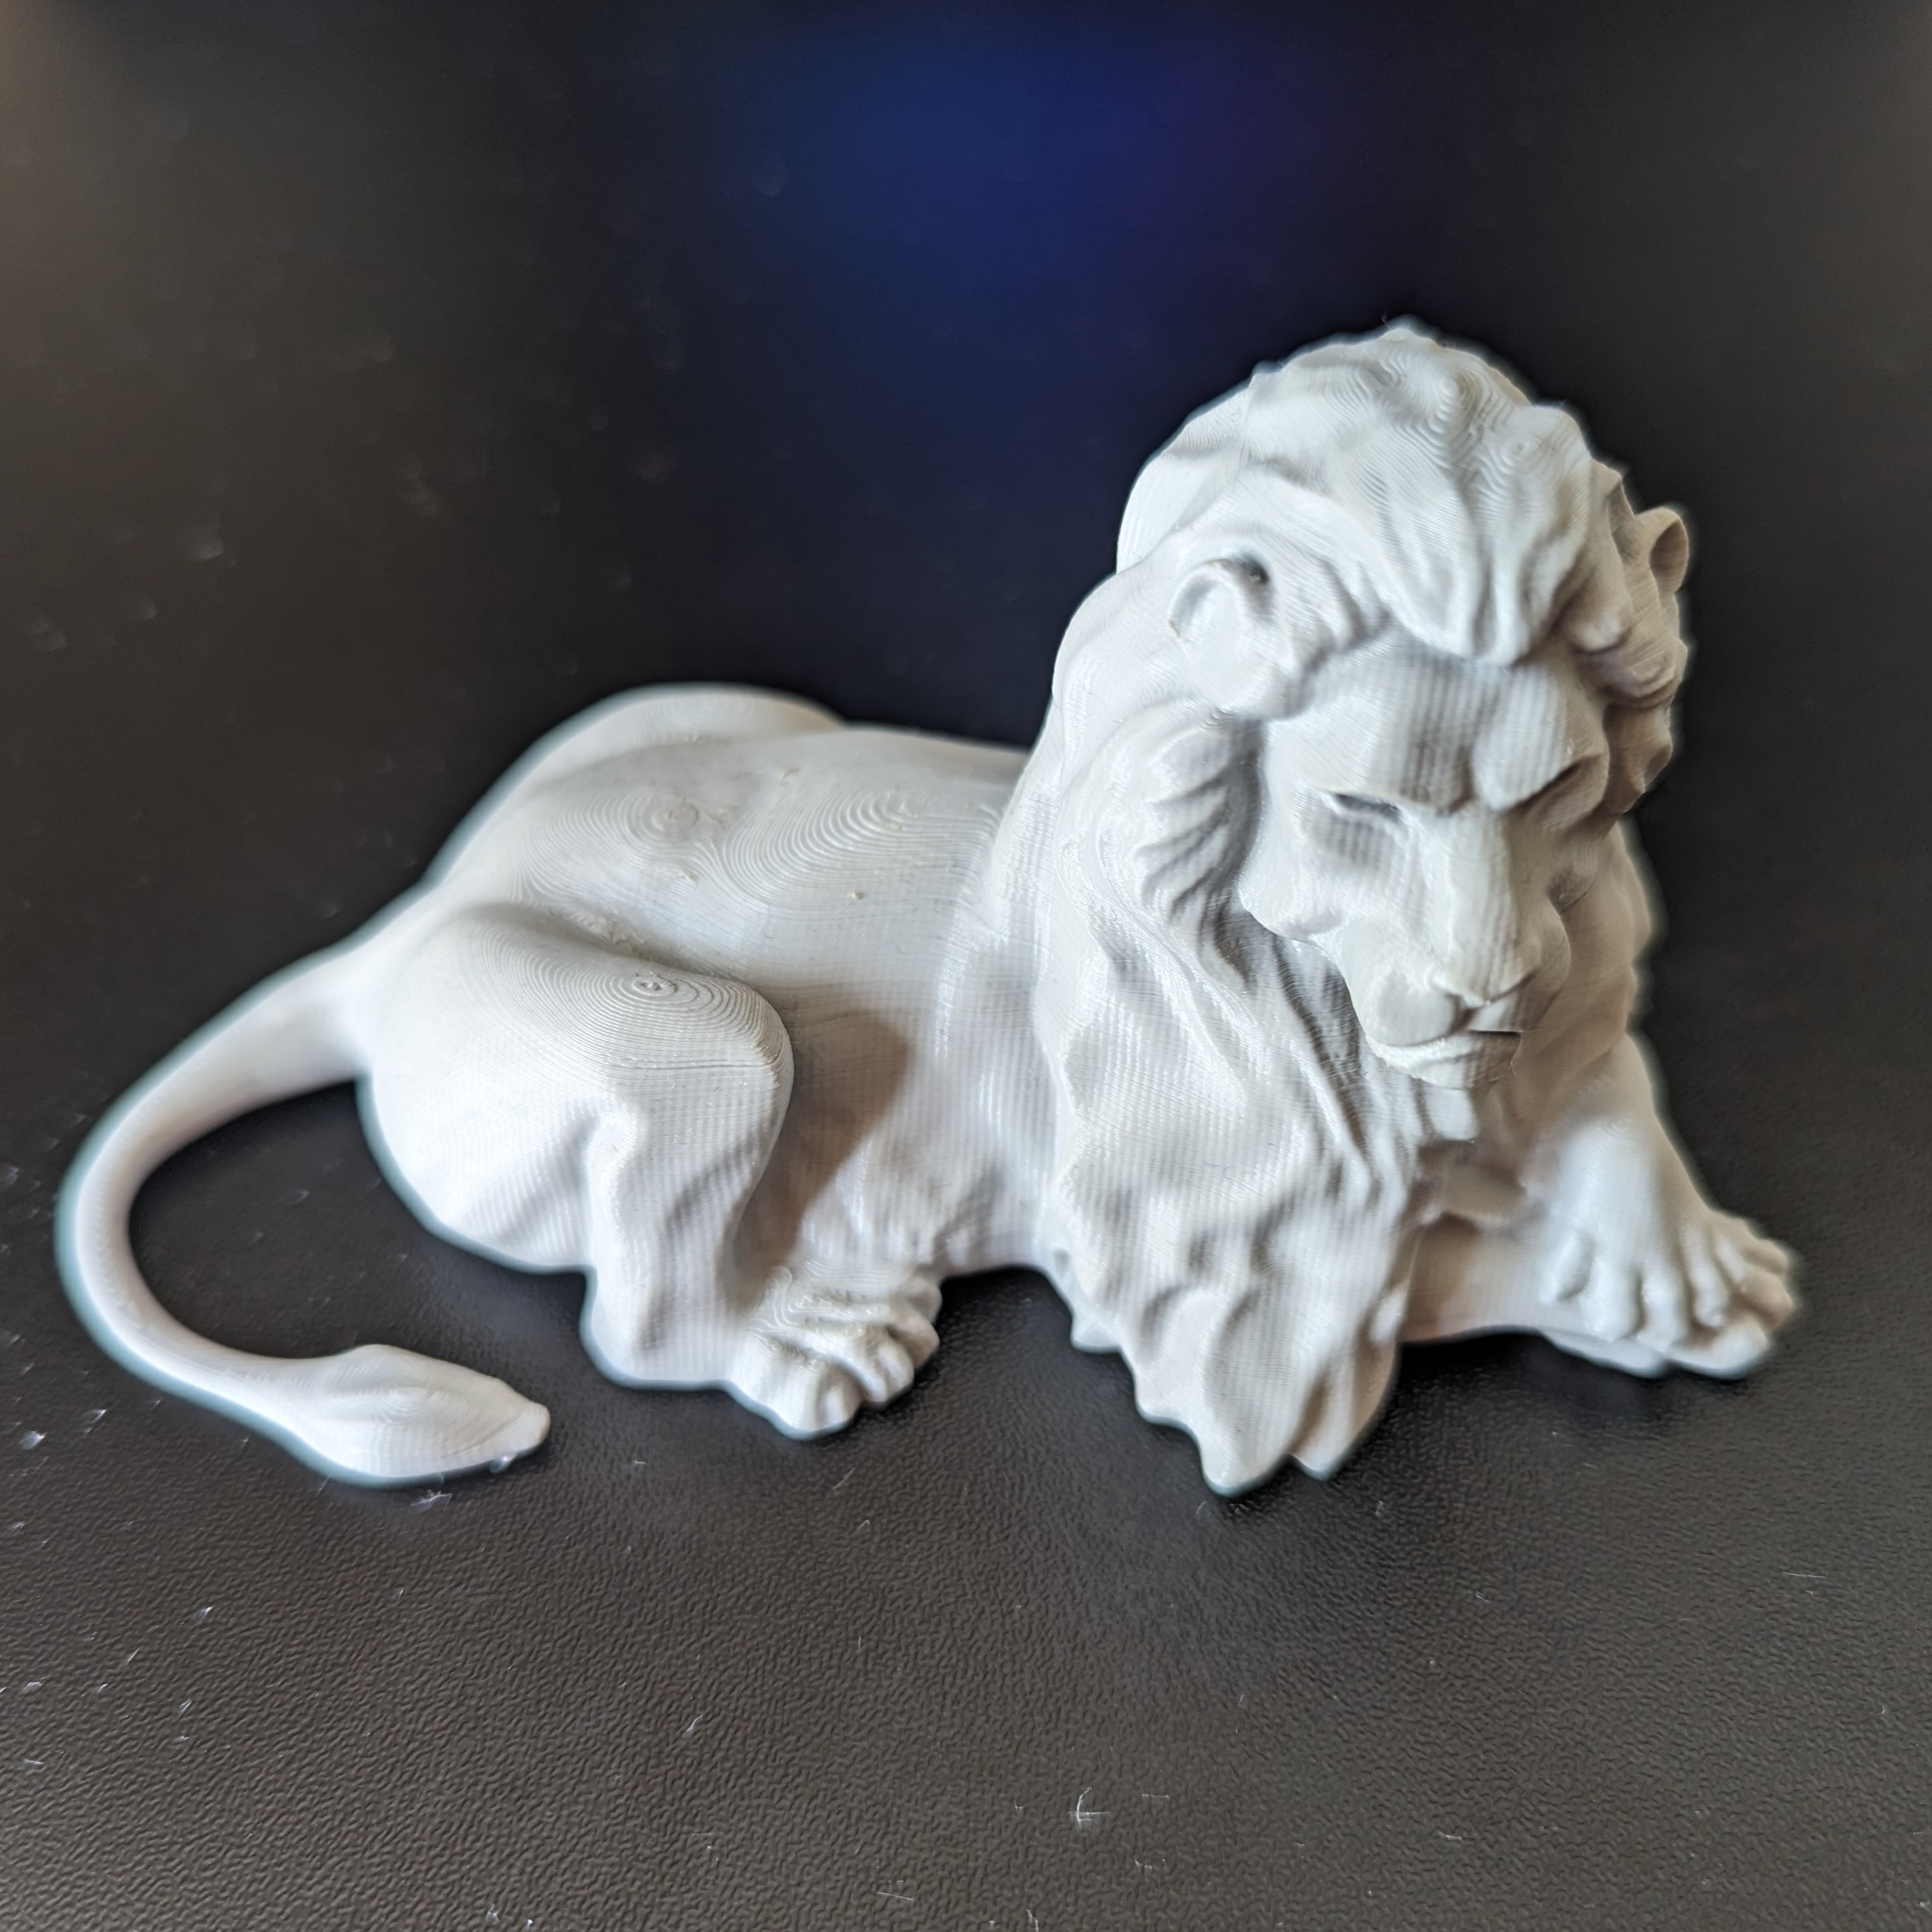
\includegraphics[width=3.4cm,height=3.4cm,keepaspectratio]{img/LionA.jpg} & 1.80 1.23 0.73 1.07 0.77 & 1.12s \\
LionB & 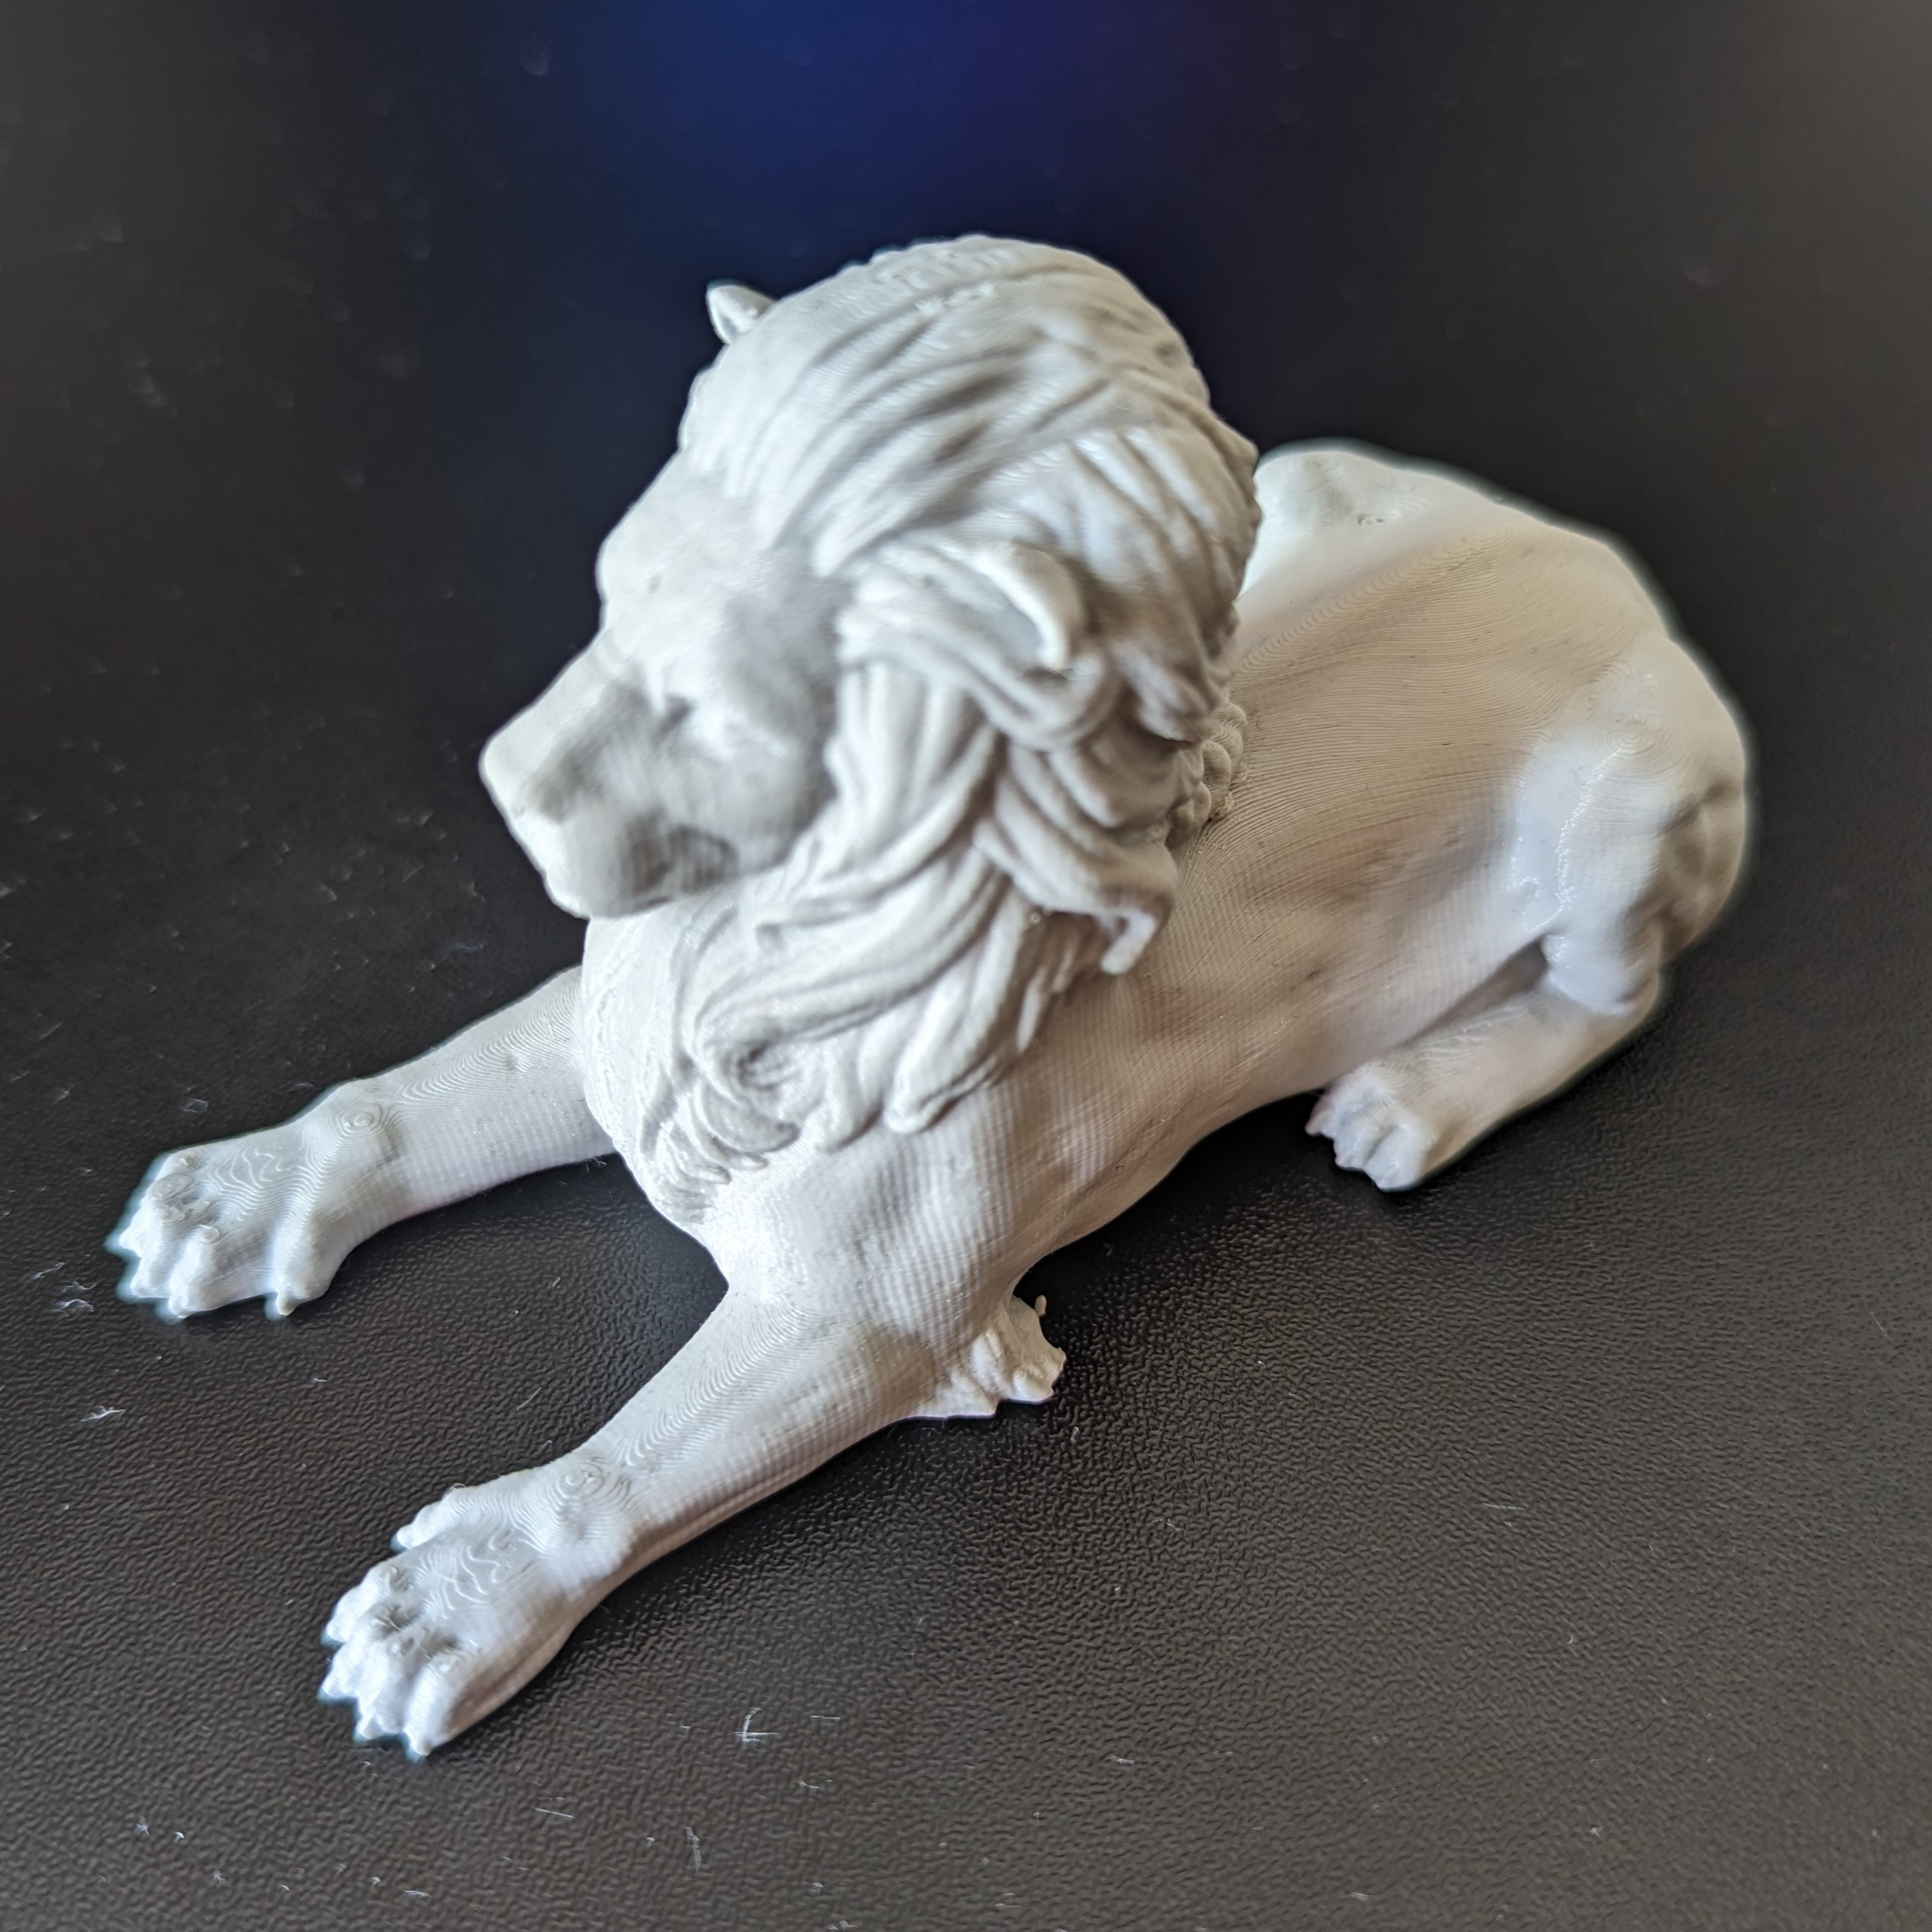
\includegraphics[width=3.4cm,height=3.4cm,keepaspectratio]{img/LionB.jpg} & 1.77 1.80 1.13 1.17 1.80 & 1.534s \\
DragonA & 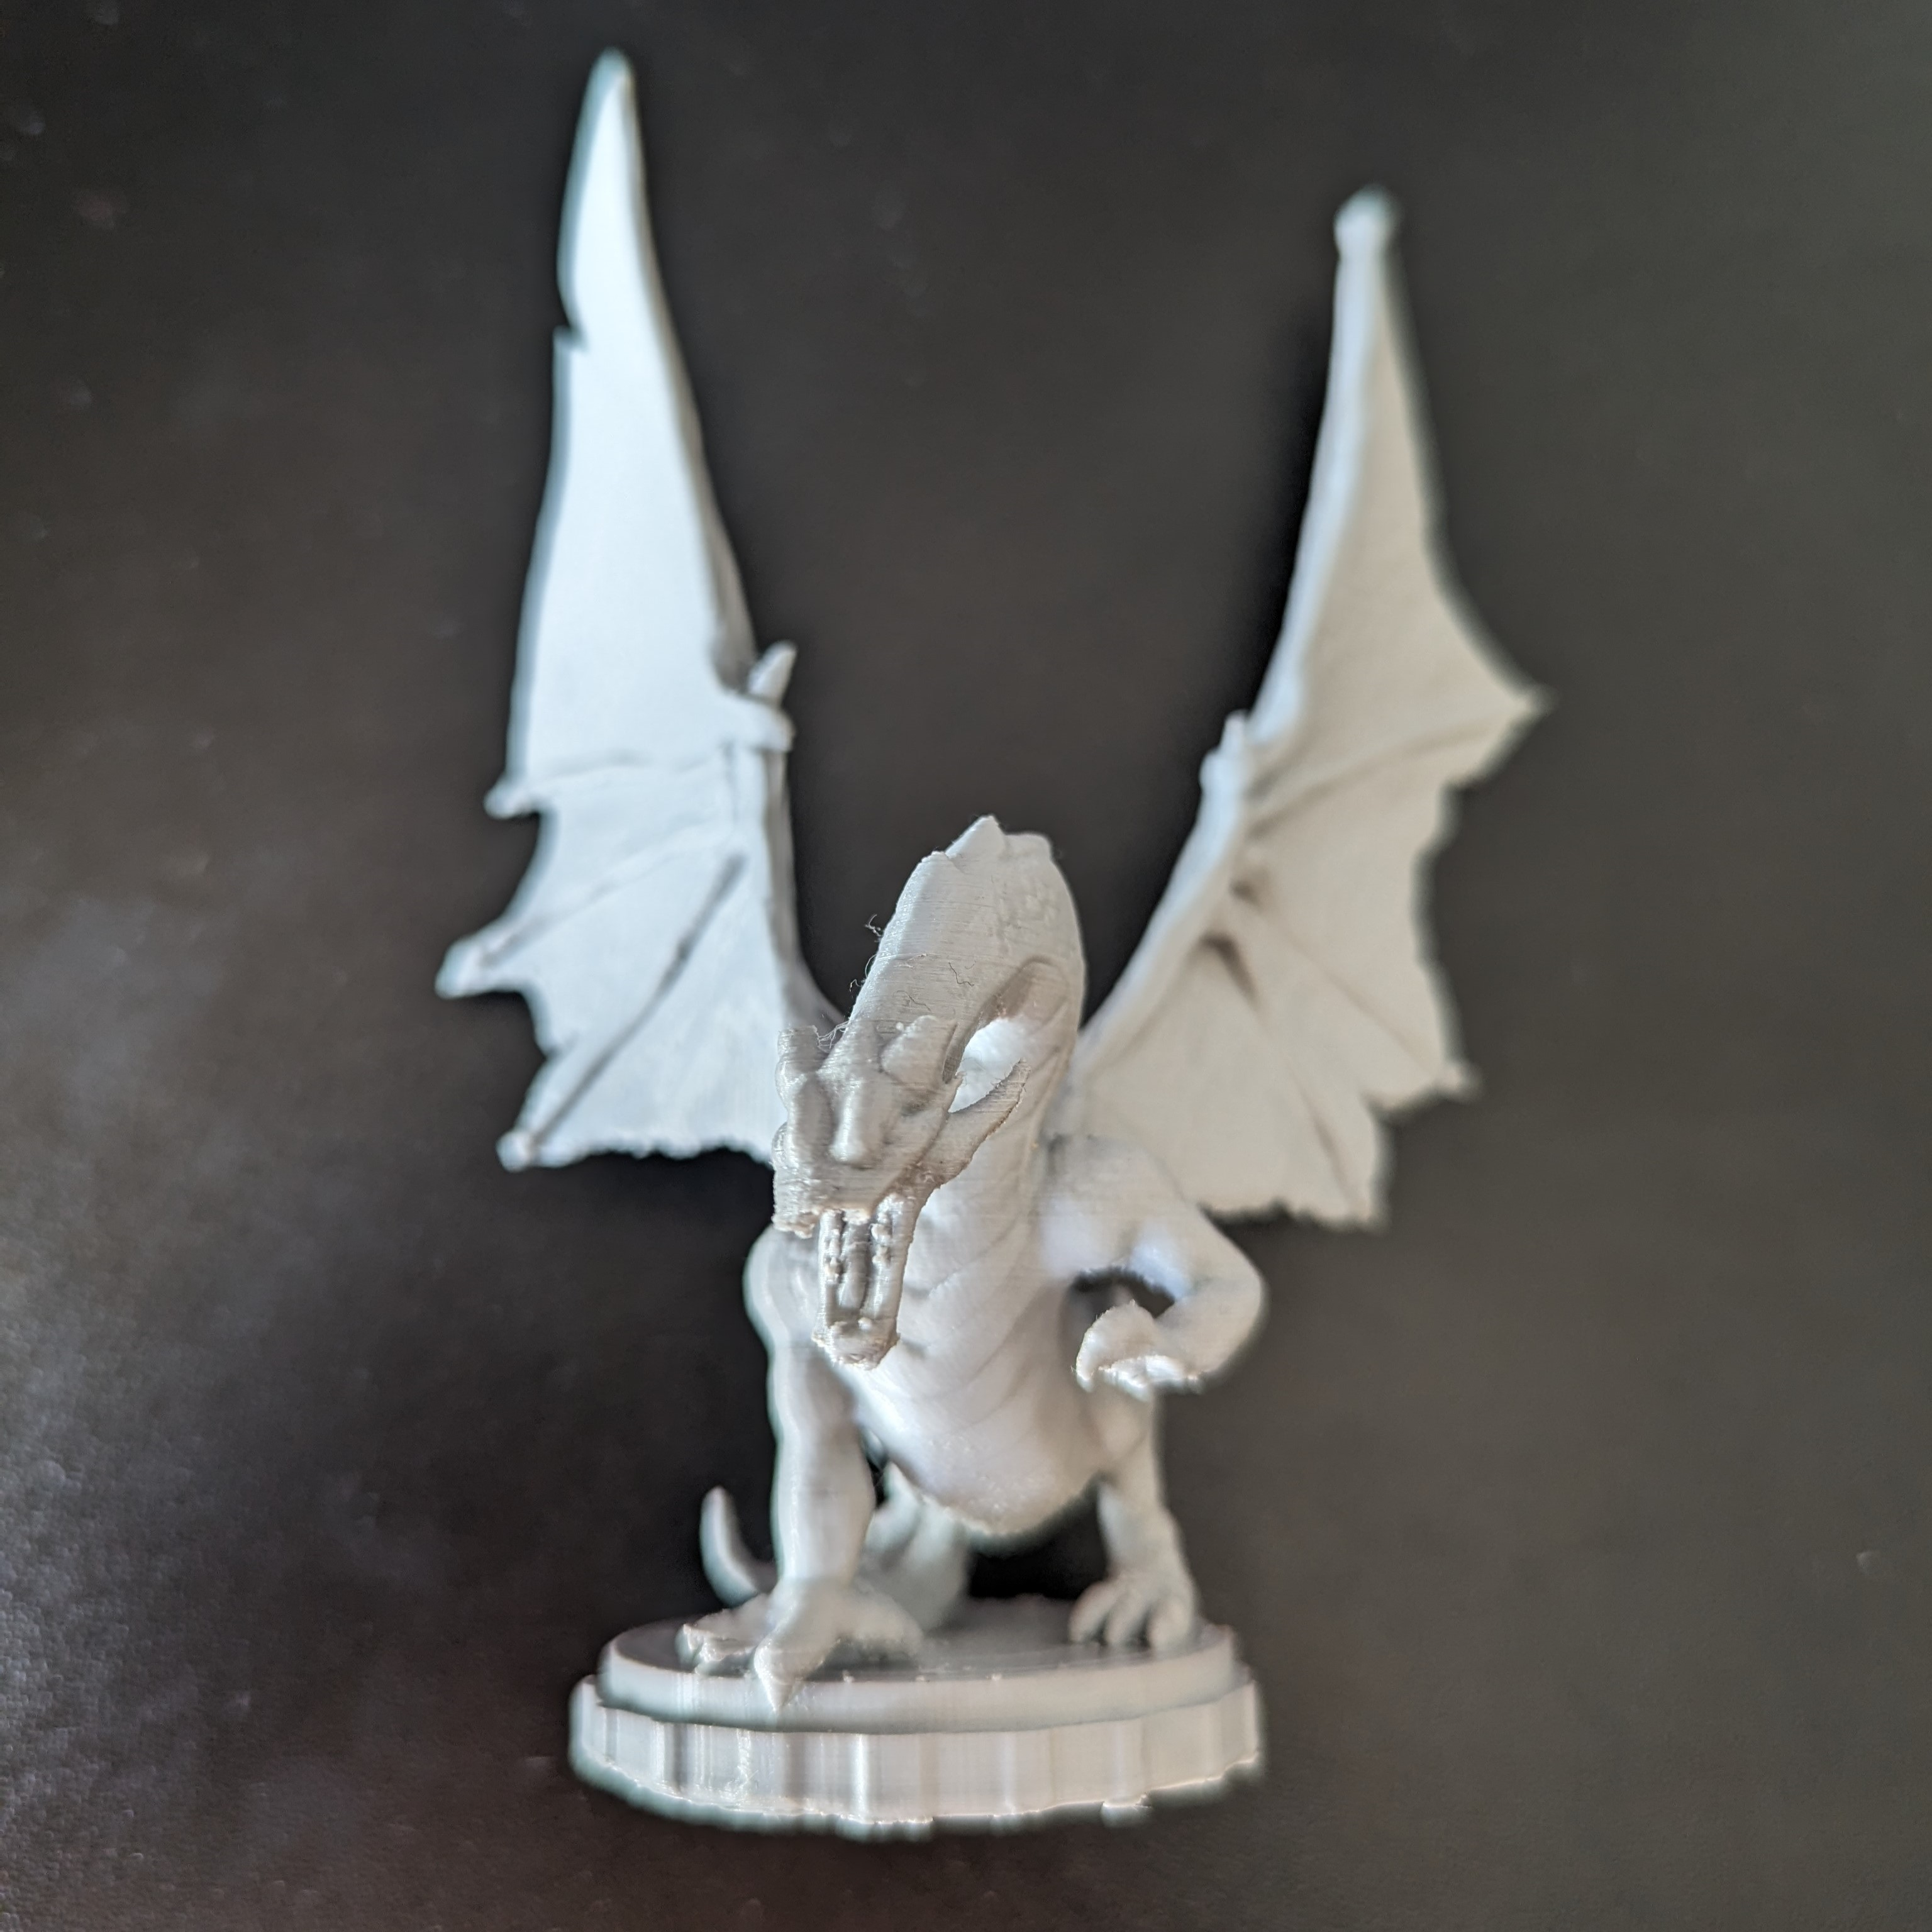
\includegraphics[width=3.4cm,height=3.4cm,keepaspectratio]{img/DragonA.jpg} & 0.90 0.87 0.83 0.73 0.87 & 0.84s \\
DragonB & 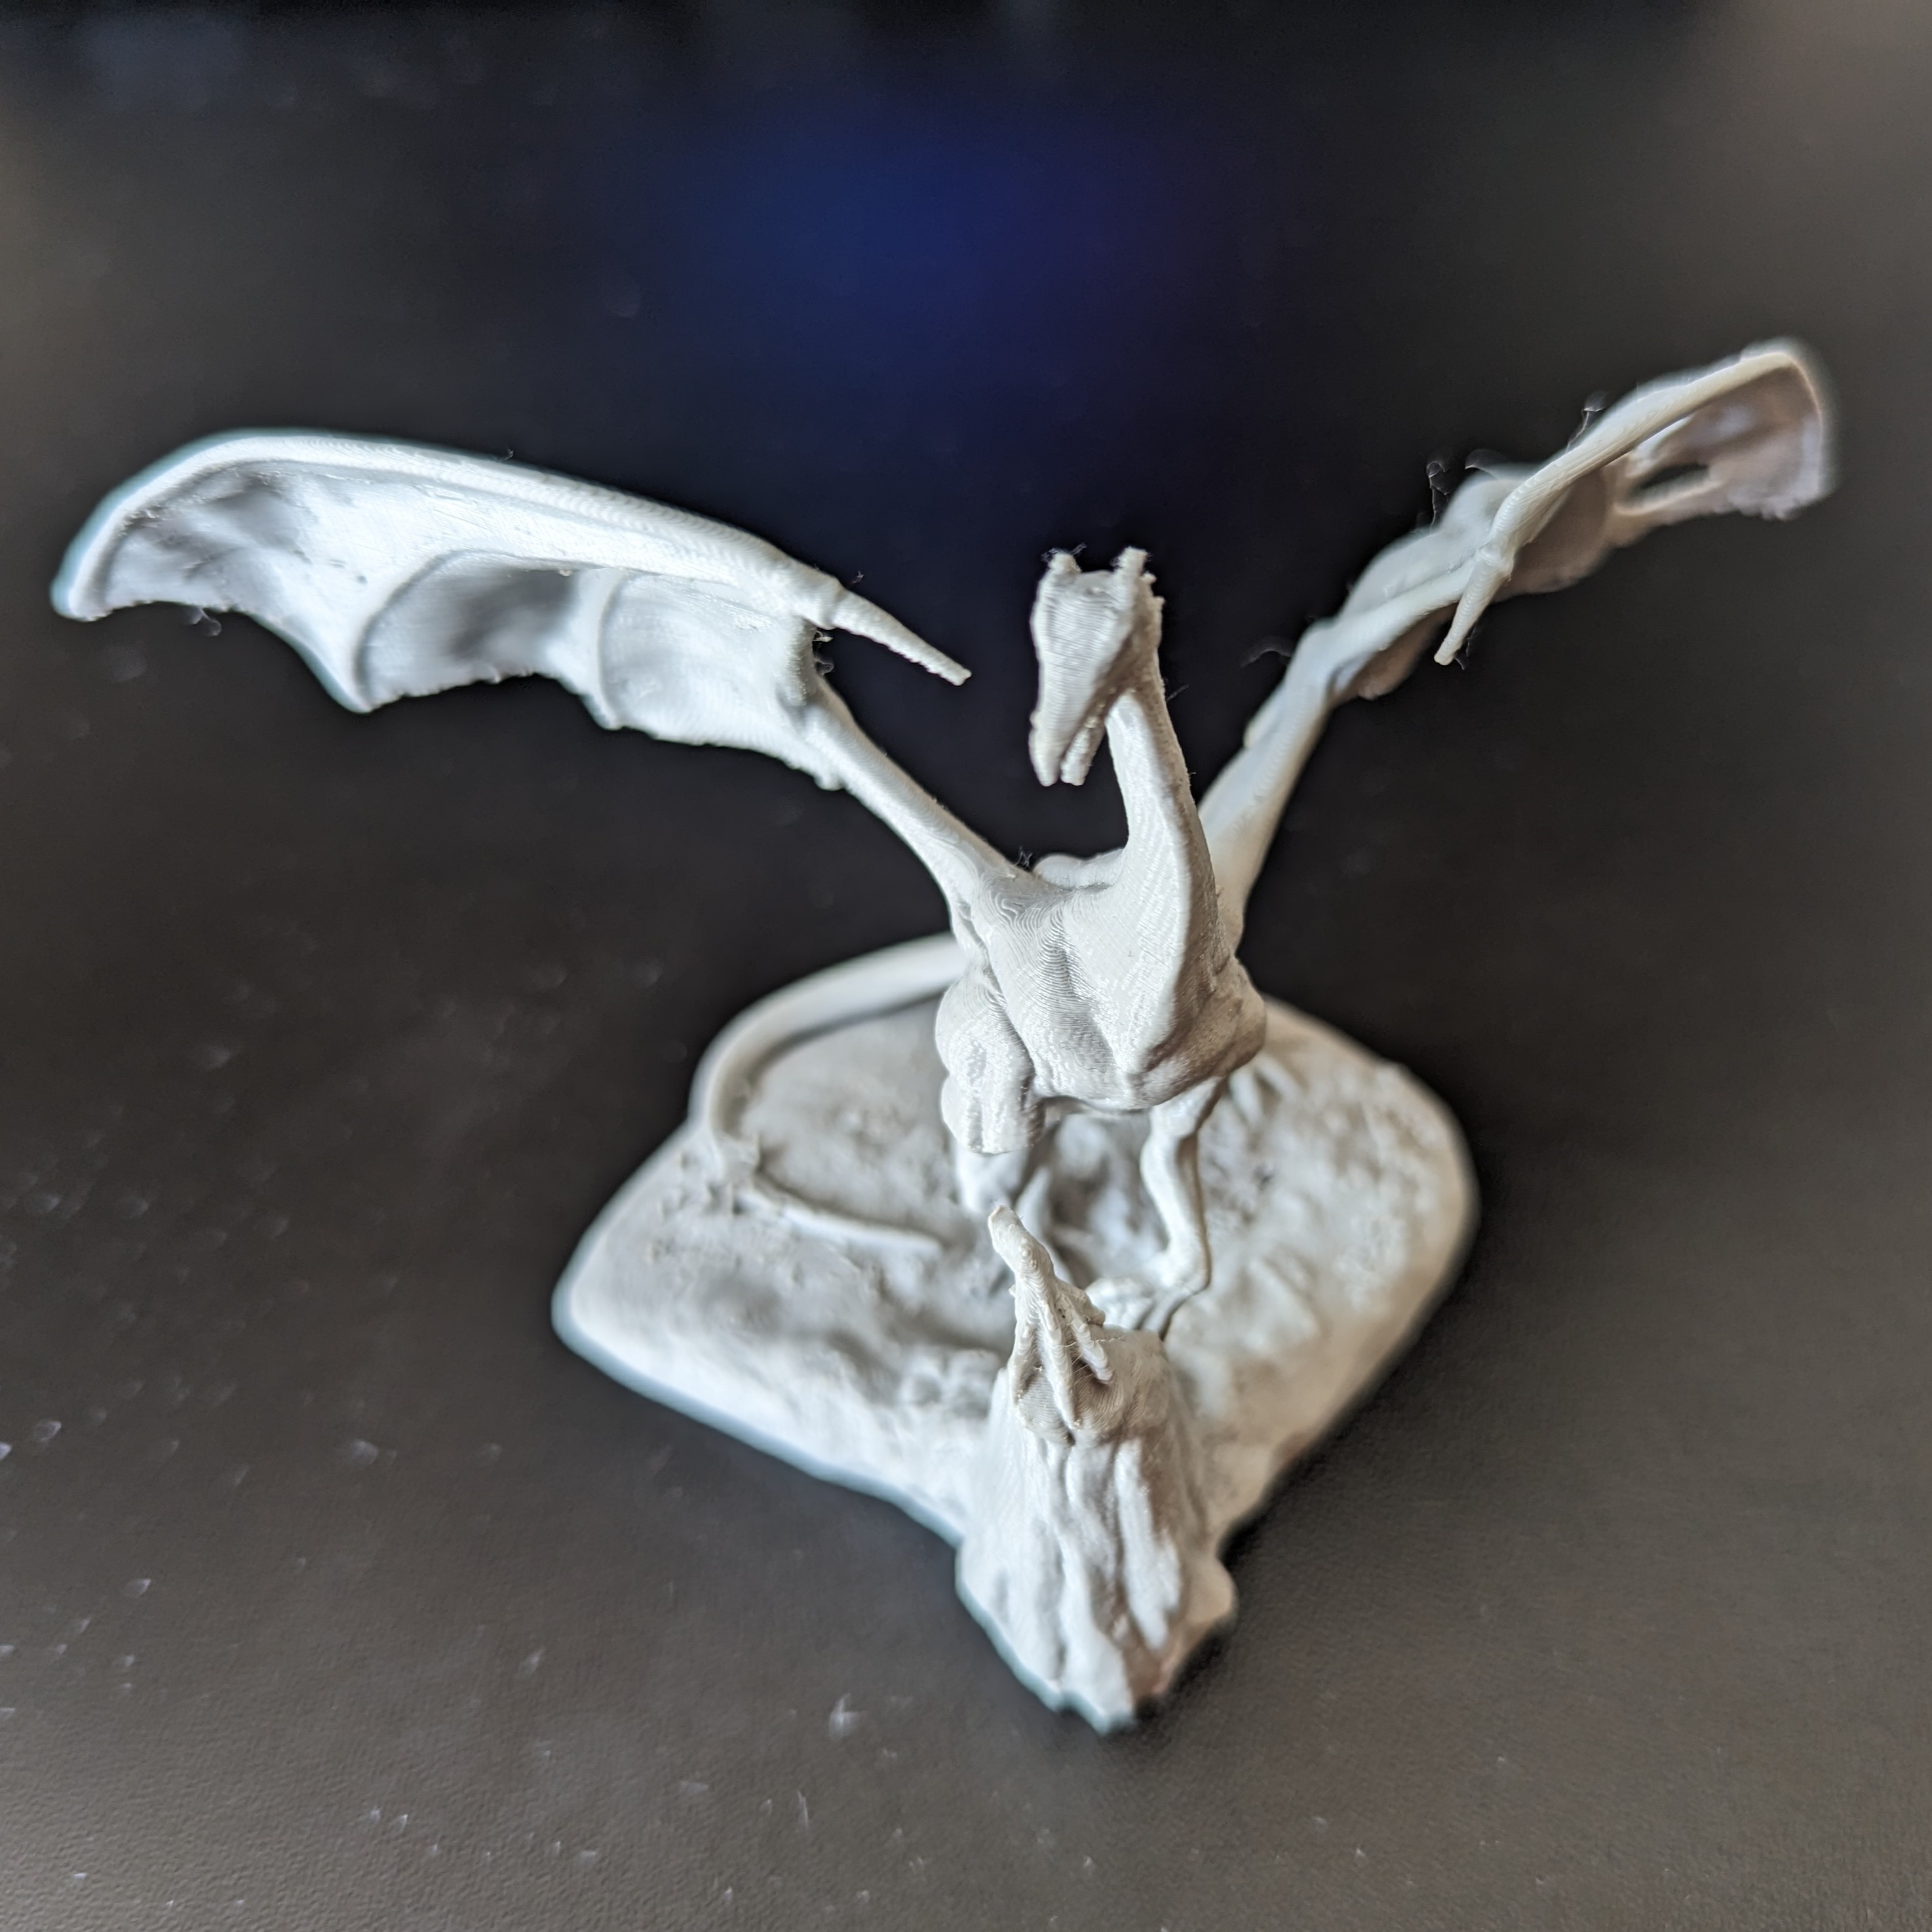
\includegraphics[width=3.4cm,height=3.4cm,keepaspectratio]{img/DragonB.jpg} & 1.70 1.77 1.77 1.73 1.80 & 1.754s \\
CubeA & 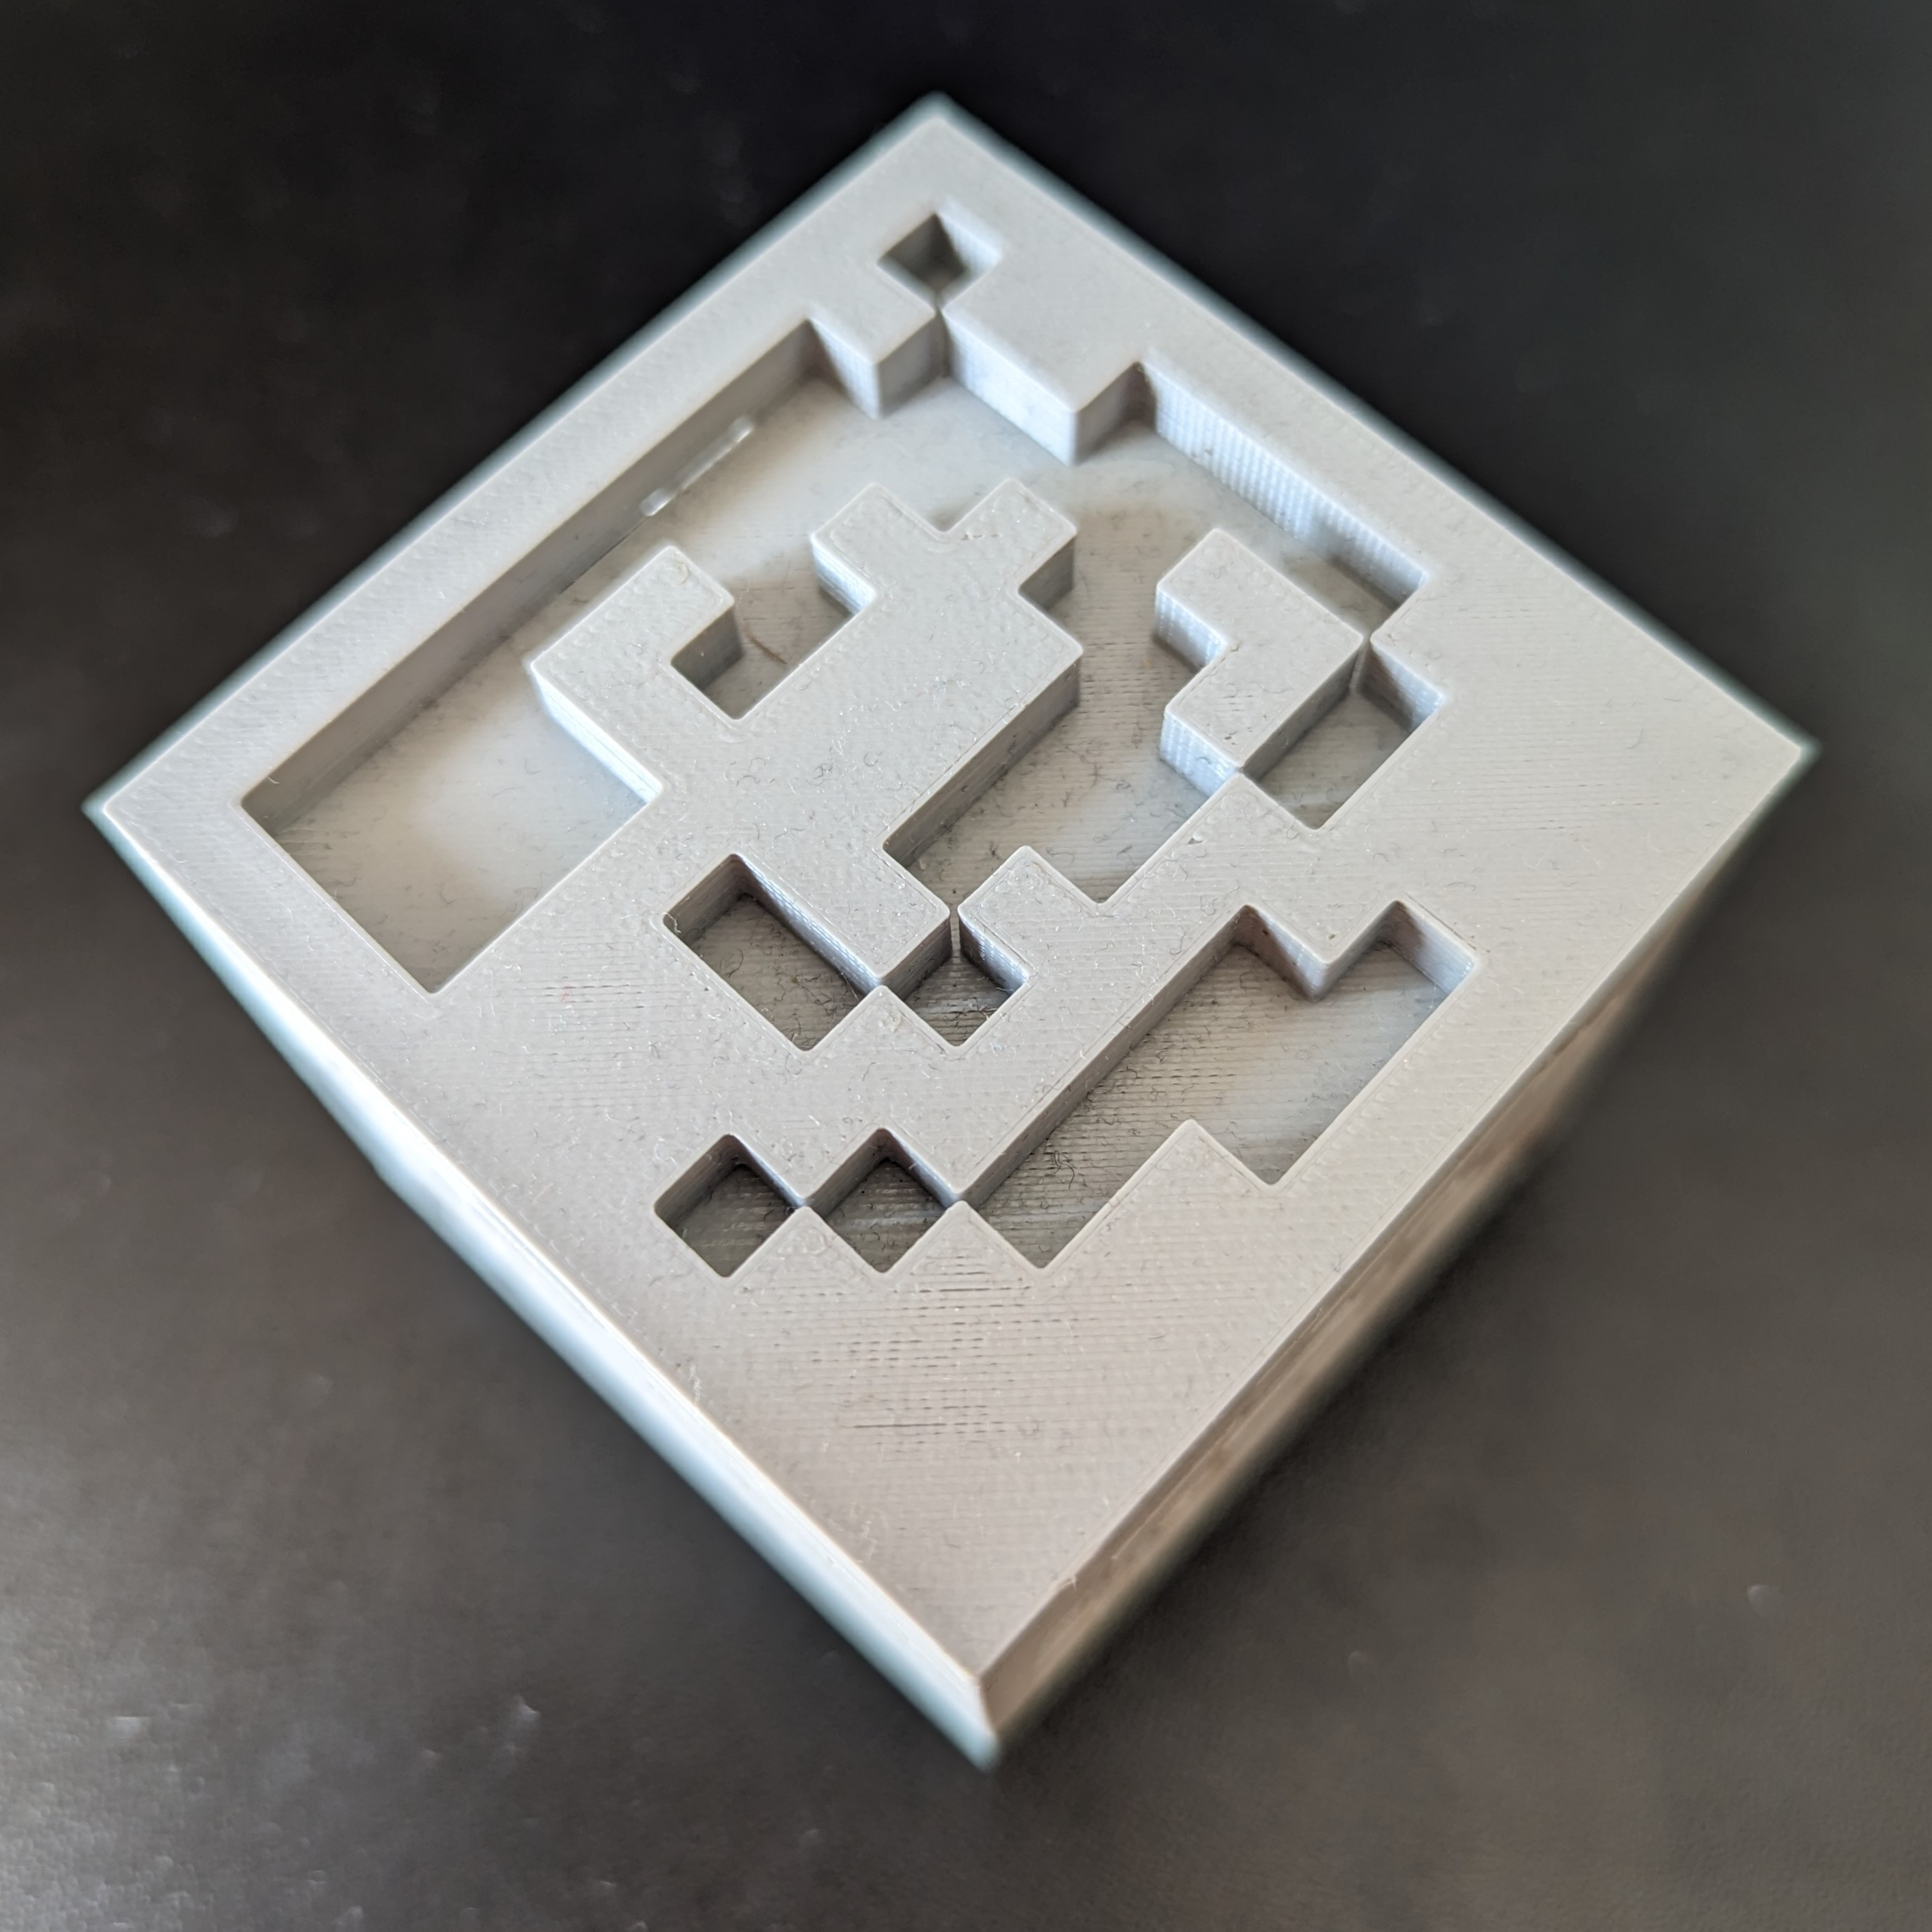
\includegraphics[width=3.4cm,height=3.4cm,keepaspectratio]{img/CubeA.jpg} & 1.70 1.83 1.67 1.77 1.77 & 1.748s \\
CubeB & 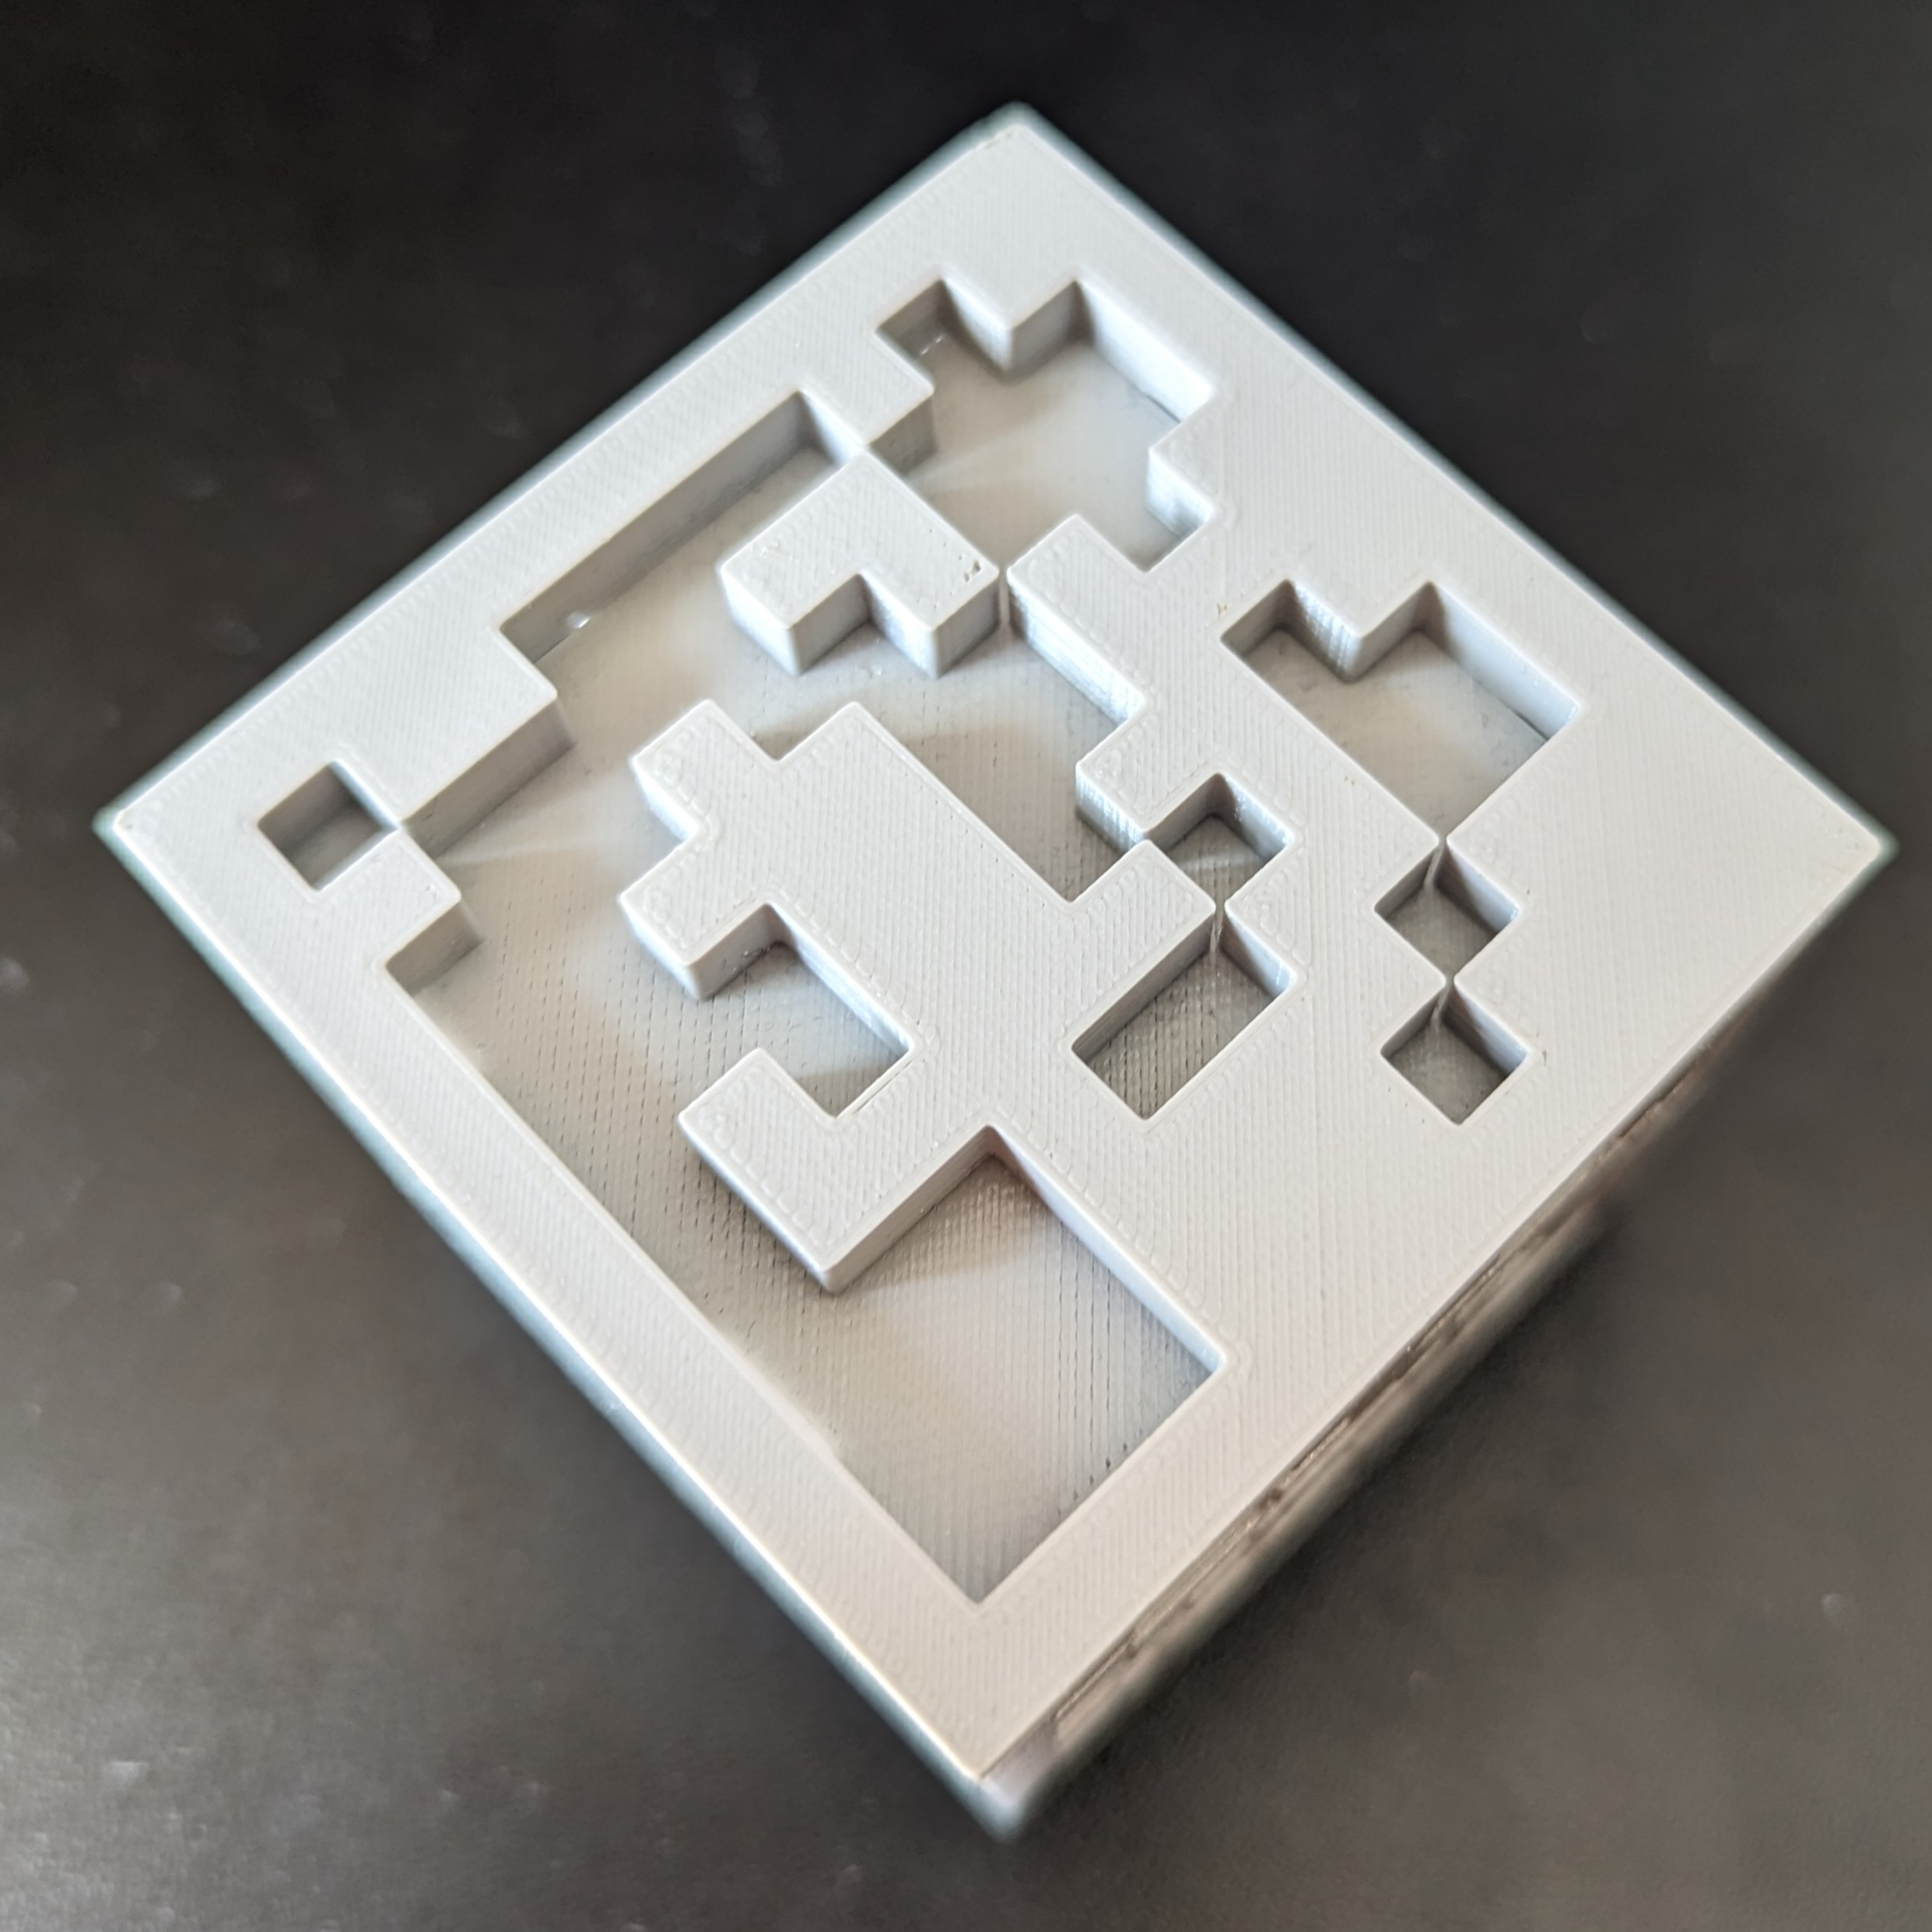
\includegraphics[width=3.4cm,height=3.4cm,keepaspectratio]{img/CubeB.jpg} & 1.80 1.80 1.77 1.77 1.43 & 1.714s \\
\hline
\end{tabular}
\end{table}